\documentclass[letterpaper,12pt,twoside]{uncthesis}

\usepackage{pgfplots}
\usepackage{tikz}
\usepackage{dcolumn}
\usepackage{soul}

\newcommand{\betrfs}{BetrFS\xspace}
\newcommand{\betrfsOne}{BetrFS 0.1\xspace}
\newcommand{\betrfsTwo}{BetrFS 0.2\xspace}
\newcommand{\betrfsThree}{BetrFS 0.3\xspace}
\newcommand{\betrfsFour}{BetrFS 0.4\xspace}
\newcommand{\betrfsFive}{BetrFS 0.5\xspace}
\newcommand{\bet}{B$^{\varepsilon}$-tree\xspace}
\newcommand{\bets}{B$^{\varepsilon}$-trees\xspace}
\newcommand{\btree}{B-tree\xspace}
\newcommand{\btrees}{B-trees\xspace}
\newcommand{\fti}{\textit{ft-index}\xspace}
\newcommand{\Fti}{\textit{Ft-index}\xspace}
\newcommand{\klibc}{\textbf{klibc}\xspace}
\newcommand{\Klibc}{\textbf{Klibc}\xspace}
\newcommand{\mdb}{\texttt{meta\_db}\xspace}
\newcommand{\ddb}{\texttt{data\_db}\xspace}
\newcommand{\spre}{\textit{src\_prefix}\xspace}
\newcommand{\dpre}{\textit{dst\_prefix}\xspace}
\newcommand{\goto}{\texttt{GOTO}\xspace}
\newcommand{\putm}{\texttt{PUT}\xspace}
\newcommand{\delm}{\texttt{DEL}\xspace}
\newcommand{\rdm}{\texttt{RD}\xspace}
\newcommand{\delold}{\textit{del\_old}\xspace}
\newcommand{\bedag}{B$^{\varepsilon}$-DAG\xspace}
\newcommand{\bedags}{B$^{\varepsilon}$-DAGs\xspace}
\newcommand{\xf}{\texttt{xf}\xspace}

\pgfkeys{
    /fs-names/ext4/.initial=ext4,
    /fs-names/btrfs/.initial=Btrfs,
    /fs-names/btrfs-svol/.initial=Btrfs-svol,
    /fs-names/xfs/.initial=XFS,
    /fs-names/zfs/.initial=ZFS,
    /fs-names/nilfs2/.initial=NILFS2,
    /fs-names/betrfs3/.initial=\betrfsThree,
    /fs-names/betrfs3-max/.initial=\betrfsThree with an infinite zone size,
    /fs-names/betrfs4/.initial=\betrfsFour,
    /fs-names/betrfs5/.initial=\betrfsFive,
}

\pgfkeys{
    /fs-colors/ext4/.initial=blue,
    /fs-colors/btrfs/.initial=red,
    /fs-colors/btrfs-svol/.initial=brown,
    /fs-colors/xfs/.initial=green,
    /fs-colors/zfs/.initial=purple,
    /fs-colors/nilfs2/.initial=cyan,
    /fs-colors/betrfs3/.initial=yellow,
    /fs-colors/betrfs3-max/.initial=orange,
    /fs-colors/betrfs4/.initial=orange,
    /fs-colors/betrfs5/.initial=gray,
}

\pgfkeys{
    /fs-marks/ext4/.initial=triangle*,
    /fs-marks/btrfs/.initial=pentagon*,
    /fs-marks/btrfs-svol/.initial=triangle*,
    /fs-marks/xfs/.initial=square*,
    /fs-marks/zfs/.initial=diamond*,
    /fs-marks/nilfs2/.initial=o,
    /fs-marks/betrfs3/.initial=+,
    /fs-marks/betrfs3-max/.initial=oplus,
    /fs-marks/betrfs4/.initial=oplus,
    /fs-marks/betrfs5/.initial=*,
}

\pgfplotsset{
    discard if/.style 2 args={
        x filter/.code={
            \edef\tempa{\thisrow{#1}}
            \edef\tempb{#2}
            \ifx\tempa\tempb
            \def\pgfmathresult{inf}
            \fi
        }
    },
    discard if not/.style 2 args={
        x filter/.code={
            \edef\tempa{\thisrow{#1}}
            \edef\tempb{#2}
            \ifx\tempa\tempb
            \else
            \def\pgfmathresult{inf}
            \fi
        }
    }
}

\newtheorem{invariant}{Invariant}


%%%%%%%%%%%%%%%%%%%%%%%%%%%%%%%%%%%%%%%%%%%%%%%%%%%%%%%%%%%%
% Required thesis information
%%%%%%%%%%%%%%%%%%%%%%%%%%%%%%%%%%%%%%%%%%%%%%%%%%%%%%%%%%%%

% When indicating your degree in the second bracketed space, use the full
% degree name (i.e., Doctor of Philosophy, not Ph.D. or PHD; Master of Public
% Health, not M.P.H. or MPH; Master of Social Work, not M.S.W. or MSW).
\uncdegreename{Doctor of Philosophy}

% List your department, school, or curriculum rather than your subject area or
% specialty discipline in the third bracketed space. You may include your
% subject area or specialty discipline in parentheses (i.e., Department of
% Romance Languages (French); School of Pharmacy (Molecular Pharmaceutics);
% School of Education (School Psychology); or similar official area).
% If you wish to include both your department and school names, list the school
% at the end of the statement (i.e., Department of Pharmacology in the School
% of Medicine).
\uncthesisdepartment{Department of Computer Science}

% Type can be dissertation or thesis
\uncthesistype{dissertation}

% Title
\uncthesistitle{Efficient, Locality-Maintaining Namespace Operations in a Write-Optimized File System}

% Name
\uncthesisauthor{Yang Zhan}

% University Name
\uncthesisuniversity{University of North Carolina at Chapel Hill}

% The year in which your committee approves the completed thesis or
% dissertation. This need not be the year you graduate.
\uncthesisyear{2019}

% Thesis advisor. Appears on the abstract page.
\uncthesisadvisor{Donald E. Porter}

% Thesis committee. Appears on the title page.  Do not include titles such as
% Professor, Doctor, Dr., PhD, or any identifiers such as “chair” or “advisor”
% before or after any names.  Put a new line after each name to render
% correctly on title page.
\uncthesiscommittee{Donald E. Porter\\
Leonard McMillan\\
F. Donelson Smith\\
Rob Johnson\\
Ethan L. Miller
}

%%%%%%%%%%%%%%%%%%%%%%%%%%%%%%%%%%%%%%%%%%%%%%%%%%%%%%%%%%%%
% Font selection
%%%%%%%%%%%%%%%%%%%%%%%%%%%%%%%%%%%%%%%%%%%%%%%%%%%%%%%%%%%%
% Font, if using PDFLaTeX
\usepackage{times}
% Font, if using XeLaTeX
%\usepackage{fontspec}
%\setmainfont{Times New Roman}

% Prevent awkward hyphenations.
\hyphenation{Raj-kumar}

\begin{document}
% The following order of the contents is REQUIRED
\pagenumbering{roman}


% 1. Title Page
\newgeometry{left=\uncthesisleftmargin in,top=2in,right=\uncthesisrightmargin in,bottom=1in,nohead}

\begin{titlepage}

\begin{singlespace}
\centering

\currentpdfbookmark{TITLE}{bk:title}

\vspace{1in}
\begin{adjustwidth}{0.5in}{0.5in}
\centering
\MakeUppercase{\uncthesistitle}
\end{adjustwidth}

\nointerlineskip\vspace{1in}

\uncthesisauthor{}

\nointerlineskip\vspace{1in}

\noindent
A \uncthesistype{} submitted to the faculty at the \uncthesisuniversity{} in partial fulfillment of the requirements for the degree of \uncdegreename{} in the \uncthesisdepartment{}.

\nointerlineskip\vspace{1in}

Chapel Hill\\
\uncthesisyear{}
%\the\year

\end{singlespace}

% Use the following block if you want the committee members to have exactly a 1in margin to the right.
%\nointerlineskip\vspace{0.83in}
%\setlength\topsep{0pt}
%\begin{flushright}
%{
%\setlength{\tabcolsep}{0pt}
%\begin{tabular}[t]{l}
%Approved by: \\
%\thesismembers
%\end{tabular}
%} % large
%\end{flushright}

% Use the following block if you want the committee members to appear approximately 2/3 the way across the page.
\nointerlineskip\vspace{0.71in}
\begin{flushright}
\begin{minipage}{2.1in}
\setlength{\tabcolsep}{0em}
\begin{tabular}{l}
Approved by: \\
\uncthesiscommittee{}
\end{tabular}
\end{minipage}
\end{flushright}

\end{titlepage}


% 2. Copyright Page (optional)
%\newgeometry{left=\uncthesisleftmargin in,top=8.42in,right=\uncthesisrightmargin in,bottom=1in,nohead}

\begin{center}
\begin{singlespace}
\copyright~\uncthesisyear\\
\uncthesisauthor \\
ALL RIGHTS RESERVED
\end{singlespace}
\end{center}

\clearpage
\newgeometry{left=\uncthesisleftmargin in,top=2in,right=\uncthesisrightmargin in,bottom=1in,nohead}
% Normal pages from here on out; TOC title takes care of 2in requirement.
\restoregeometry


% 3. Abstract
\begin{abstract}

There seems to be a trade-off between good locality and efficient namespace
operations in file systems.
Traditional inode-based file systems have good rename performance, but fail
to maintain locality, especially in the face of file system aging.
On the other hand, full-path-indexed file systems ensure locality, however,
renaming a directory needs to update all related full-paths,
which is usually implemented as an expensive operation.

This dissertation describes a technique that has both good locality and
efficient namespace operations.
In particular, we describe a novel synthesis of write-optimization,
full-path indexing and operations on data structures.
By directly manipulating the data structure, a full-path-indexed file system
can efficiently update related full-paths in a rename.
Moreover, with the technique, a full-path-indexed file system can
clone a directory without traversing the directory.

We implement this technique in \betrfs, a full-path-indexed, write-optimized,
local file system for Linux.
Compared to ext4, the widely used inode-based file system in Linux,
the new version of \betrfs traverses the Linux source directory 9.47x faster,
and renames the same directory 1.09x faster.
Meanwhile, the new version of \betrfs clones a directory faster than
file systems that clone the directory through file clones,
such as Btrfs and XFS.

\end{abstract}


% 4. Dedication, Acknowledgement(s), Preface (each optional)
%\begin{dedication}
A dedication is a message from the author prefixed to a work in tribute to a person, group, or cause. Most dedications are short statements of tribute beginning with \textit{``To \ldots''} such as \textit{``To my family''}.
\end{dedication}

\begin{acknowledgement}

acks

\end{acknowledgement}

%\begin{preface}

A preface is a statement of the author's reasons for undertaking the work and other personal comments that are not directly germane to the materials presented in other sections of the thesis or dissertation. These reasons tend to be of a personal nature.

    \lipsum[6]

\end{preface}


% 5. Table of Contents, with page references
\renewcommand{\contentsname}{\hfill\bfseries\normalsize TABLE OF CONTENTS\hfill}
%\renewcommand{\cfttoctitlefont}{\hfill\Large\bfseries}
\renewcommand{\cftaftertoctitle}{\hfill}
\renewcommand{\cftdotsep}{1.5}
\cftsetrmarg{1.0in}

\setlength{\cftbeforetoctitleskip}{56pt}
\setlength{\cftaftertoctitleskip}{18pt}

% format chapter entries like other entries
\renewcommand{\cftchapfont}{\normalfont}
\renewcommand{\cftchappagefont}{\normalfont}
\renewcommand{\cftchapleader}{\cftdotfill{\cftdotsep}}

\setlength{\cftbeforechapskip}{15pt}
\setlength{\cftbeforesecskip}{10pt}
\setlength{\cftbeforesubsecskip}{10pt}
\setlength{\cftbeforesubsubsecskip}{10pt}

\begin{singlespace}
\currentpdfbookmark{TABLE OF CONTENTS}{bk:contents}
\tableofcontents
\end{singlespace}

\clearpage


% 6. List of Tables, with titles and page references (if applicable). And list
% of Figures or Illustrations, with titles and page references (if applicable)
\renewcommand{\listtablename}{LIST OF TABLES}
\phantomsection
\addcontentsline{toc}{chapter}{LIST OF TABLES}

\setlength{\cftbeforelottitleskip}{-14pt}
\setlength{\cftafterlottitleskip}{22pt}
\renewcommand{\cftlottitlefont}{\hfill\normalsize\bfseries}
\renewcommand{\cftafterlottitle}{\hfill}

\setlength{\cftbeforetabskip}{12pt}
\cftsetrmarg{1.0in}

\setlength{\cfttabindent}{0in}

\begin{singlespace}
\listoftables
\end{singlespace}

\clearpage

\renewcommand{\listfigurename}{LIST OF FIGURES}
\phantomsection
\addcontentsline{toc}{chapter}{LIST OF FIGURES}

\setlength{\cftbeforeloftitleskip}{-14pt}
\setlength{\cftafterloftitleskip}{22pt}
\renewcommand{\cftloftitlefont}{\hfill\normalsize\bfseries}
\renewcommand{\cftafterloftitle}{\hfill}

\setlength{\cftbeforefigskip}{12pt}
\cftsetrmarg{1.0in}

\setlength{\cftfigindent}{0in}

\begin{singlespace}
\listoffigures
\end{singlespace}

\clearpage


% 7. List of Abbreviations (if applicable)
\phantomsection
\addcontentsline{toc}{chapter}{LIST OF ABBREVIATIONS}

\begin{center}
\textbf{LIST OF ABBREVIATIONS}
\vspace{16pt}
\end{center}

% TODO: define new column types to make sure multi-line table cells has single-spacing

\noindent
\begin{tabular}{p{0.8in} p{5in}}
LCA     & Lowest Common Ancestor\\
LCP     & Longest Common Prefix\\
VFS     & Virtual File System\\
WOD     & Write-Optimized Dictionary\\
\end{tabular}

\clearpage


% 8. List of Symbols (if applicable)
%\phantomsection{}
\addcontentsline{toc}{chapter}{LIST OF SYMBOLS}

\begin{center}
\textbf{LIST OF SYMBOLS}
\vspace{16pt}
\end{center}

\noindent
\begin{tabular}{@{}p{0.8in} l}
$M$ & Number of wands\\
$m$ & Number of wizards\\
$n$ & Number of fantastic beasts\\
\end{tabular}

\clearpage


\pagenumbering{arabic}

%\chapter{Formatting Guide}
\label{chap:formatting_guide}

\section{Margins}

This template follows the UNC graduate school thesis/dissertation formatting guide as rigidly as possible.
This template has uniform margins throughout the entire document:
\begin{itemize}
    \item Left: 1''
    \item Right: 1''
    \item Top: 1''
    \item Bottom: 1''
\end{itemize}

\section{Font}
A TrueType font is recommended/required by the ProQuest dissertation publishing. Recommended fonts and sizes can be found in \autoref{tab:font}.

\begin{table}
    \centering
    \caption{Recommended font type and size}\label{tab:font}
    \begin{tabular}{ll}
        \toprule
        Font name            & Font Size \\ \midrule
        Arial                & 10pt\\
        Century              & 11pt\\
        Courier New          & 10pt\\
        Garamond             & 12pt\\
        Georgia              & 11pt\\
        Lucida Bright        & 10pt\\
        Microsoft Sans Serif & 10pt\\
        Tahoma               & 10pt\\
        Times New Roman      & 12pt\\
        Trebuchet MS         & 10pt\\
        Verdana              & 10pt\\ \bottomrule
    \end{tabular}
\end{table}

If you're using \texttt{pdflatex} to compile this template, include the \texttt{times} package in the preamble.
If you're using \texttt{xelatex} to compile this template, you can use the \texttt{fontspec} package and the \texttt{setmainfont} command to choose your favorite font.
This template by default uses 12pt Times New Roman.

\section{Spacing and Indentation}

The template takes care of spacing and indentation:
\begin{itemize}
    \item Text appears in a single column on each page and is double-spaced throughout the document.
    \item New paragraphs are indicated by a consistent tab indentation throughout the entire document.
    \item The document text is left-justified.
    \item For blocked quotations, indent the entire text of the quotation consistently from the left margin.
\end{itemize}

\lipsum[6]
\begin{quote}
    This is an example showing the indentation of block quoted text.
    \lipsum[8]
\end{quote}
\lipsum[7]

\section{Pagination}
This template takes care of pagination.

Pagination and margin are also well maintained for landscape pages.
\begin{landscape}
    \lipsum[9] Let's also see how does footnote works in landscape pages~\footnote{We have a footnote in landscape environment}.
\end{landscape}

\section{Footnotes and Endnotes}
Footnotes\footnote{\lipsum[10]} and endnotes\footnote{\lipsum[11]} obey the
formatting guide. However, using both of them confuses the note numbering.
Given the discrepancy between the official format guide\endnote{\lipsum[12]}
and the official sample pages\endnote{\lipsum[14]}, the correct order for
endnotes and appendixes are unclear.  Thus, using only footnote is recommended.

\section{Tables and Figures}
Tables, figures, and illustrations vary widely by discipline. Therefore, formatting of these
components is largely at the discretion of the author.

List of figures and list of tables are well taken care of by \LaTeX{} and this
template.  If an entry in LOT/LOF takes up more than one line, break up the
entry about three-fourths of the way across the page and place the rest of the
text on a second line, single-spacing the two lines.

One nice trick is the short caption option for the
\texttt{\textbackslash{}caption{}} command.  It allows the LOT/LOF only include
the short caption but not the full caption.
\begin{figure}
    \centering
    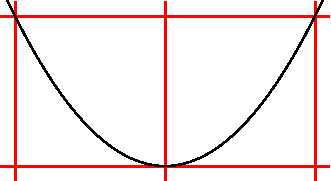
\includegraphics[width=0.5\textwidth]{figures/demo.pdf}
    \caption{A very long caption that does not make much sense but only tests the line-breaking and line-spacing in LOT/LOF.}
\end{figure}

\begin{figure}
    \centering
    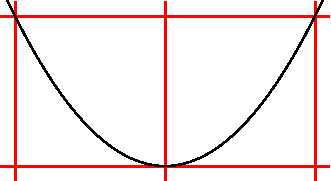
\includegraphics[width=0.5\textwidth]{figures/demo.pdf}
    \caption[Short Caption]{A very long caption that does not make much sense but only tests the line-breaking and line-spacing in LOT/LOF.}
\end{figure}

\section{Reference}
The APA style is used for references. Notice the differences caused by different citation command.

\begin{table}
    \centering
    \caption[Short title]{Comparison of different citation command.}\label{tab:citation}
    \begin{tabular}{ll}
        \toprule
Command                        & Results \\ \midrule
\texttt{\textbackslash{}cite}  & \cite{LFR}\\
\texttt{\textbackslash{}citep} & \citep{LFR}\\
\texttt{\textbackslash{}citet} & \citet{LFR}\\\bottomrule
    \end{tabular}
\end{table}

\section{Length}
There are no requirements for the length of the PhD thesis. For the Department of Computer Science, from 2014 to 2017, average length of the thesis main body text is $\mu \approx 120, \sigma \approx 33$, average length of main body text + reference is $\mu \approx 129, \sigma \approx 35$.
%\chapter{Related Works}
\label{chap:related}

\section{A very long section title testing the line-breaking and line-spacing in TOC if not long enough we make it longer}
\subsection{Subsection title}
\lipsum{}
\subsubsection{Subsubsection title}
\lipsum[1]
\subsection{Another subsection title}


\chapter{Introduction}
\label{chap:intro}

Today's general purpose file systems fail to utilize the full bandwidth of the
underlying hardware.
Widely used inode-based file systems, such as ext4, XFS, and Btrfs, can write
large files at near disk bandwidth,
but typically create small files at less than 3\% of the disk bandwidth.
Similarly, these file systems can read large files at near disk bandwidth,
but scanning directories with many small files is slow, and the performance
degrades when the file system ages~\citep{betrfs3}.

At the heart of this issue is how data is organized on disk.
The most common design pattern for modern file systems is to use multiple layers
of indirection.
The inode number of a file or directory connects the name of an entry in a
directory to its metadata location on disk.
The metadata of an inode contains extents that describes the physical location
and length of data at different offsets.
Indirection simplifies implementation of the file system, and makes some
operations, such creating files and appending files, easy to implement.
In particular, namespace operations are simple and flexible.
For example, a rename is just a pointer swing, moving an entry from one
directory to another directory.
However, indirection doesn't impose any constraint on how metadata and data
are placed on the disk.
In the worst case, the metadata of entries under a directory and the content of
a file can end up scattered over the disk.
Heuristics, such as cylinder groups~\citep{ffs1}, are designed to mitigate this
problem.
However, on modern inode-based file systems, unless the metadata or data are
modified, their location doesn't change.
Therefore, after disk space is allocated and freed over file system aging,
the free space on disk becomes scattered,
leading to bad performance for both reads and writes.

One attempt to solve the problem of random writes is the log-structured file
system~\citep{lfs}.
The log-structure file system treats the disk as a log, so small random writes
becomes log appends, which are significantly faster.
However, the log cleaner in a log-structured file system has severe impact on
performance~\citep{lfsbsd}, especially when the log is full.
And the log-structured file system still uses multiple levels of
indirection, resulting in slow directory traversals.

An alternative design is to use full-path indexing upon write-optimized
dictionaries (WODs) in a file system, known to have good performance on nearly
all operations.
On one hand, WODs have fast random write performance.
A WOD divides its data into multiple levels whose sizes grow exponentially.
Writes are put to the lowest level, and gradually merged to higher levels in
batches.
This merging process in a WOD keeps data sorted in a certain order at each level
and acts as a cleaner to garbage-collect lower levels.
On the other hand, full-path indexing ensures metadata and data in
depth-first-search order, that is, lexicographic order by the full-path names
of files and directories.
With full-path indexing, metadata and data under one directory are close to each
other in key space, which, combined with the sorted order maintained by
WODs, leads to good locality and fast directory traversals.
Prior work~\citep{betrfs1,betrfs1tos,betrfs2,betrfs2tos,betrfs3} of this design
realizes efficient implementation of many file-system operations, such as random
writes, file creates and directory traversals,
but a few operations still have prohibitively high overheads.

The Achilles' heel of such design is the performance of namespace operations,
in particular, renaming large files and directories.
For instance, renaming a large directory changes the full-paths of all files
and directories under it, which updates keys of the metadata and
data and moves them in the key space.
Competitive performance for namespace operations in full-path-indexed file
systems should complete in an I/O-efficient manner.

However, prior work mainly focuses on the schema level of the file system, i.e.,
how metadata and data are keyed and indexed in the WODs.
The full-path-indexed file system usually implements a rename by
fetching all key/value pairs of metadata and data,
inserting them back with updated keys, and deleting old key/value pairs.
Therefore, a rename needs to call several operations for each affected full-path
names, leading to bad performance.
Or, the file system partly backs away from full-path-indexing and adopts
relative-path-indexing, a hybrid of full-path-indexing and indirection.
This approach not only breaks the locality of full-path-indexing, but also
taxes other operations for efficient namespace operations.

This dissertation presents I/O-efficient ways to do namespace operations in a
full-path-indexed, write-optimized file system.
Specifically, though full-path indexing limits possible change on the schema
level, we observe that it can make all full-path names under a directory
contiguous in key space.
And the underlying WOD, \bets, has a tree structure, which makes it possible to
move or clone a contiguous key range efficiently.
Therefore, we dig into the underlying \bets, and implements two new operations,
range-rename and range-clone, that completes file system renames and clones with
bounded number of I/Os.

Chapter~\ref{chap:bg} talks about the necessary background of this dissertation.
We start with a presentation of the write-optimized \bets,
showing the idea of write-optimization.
Then, we describes full-path-indexed \betrfs and relative-path-indexed \betrfs.
The full-path-indexed \betrfs shows the benefit of full-path indexing combined
with write-optimization, but suffers from slow renames.
The relative-path-indexed \betrfs has good rename performance, but breaks the
full-path indexing and taxes other operations for efficient renames.

Chapter~\ref{chap:rename} presents the range-rename operation on \bets,
which full-path-indexed \betrfs can use to implement file system renames.
A range-rename updates all keys with one prefix to another prefix efficiently
through two techniques, \textbf{key lifting} and \textbf{tree surgery}.

Chapter~\ref{chap:clone} expands range-rename to range-clone,
which full-path-indexed \betrfs can use to implement both file or directory
renames and clones.
We first show how to implement range-clone with range-rename techniques by
transforming \bets into \bedags.
Then, we introduces a new type of messages, \goto messages, that works as other
messages in \bedags, fitting range-clone into write-optimization.

Chapter~\ref{chap:eval} evaluates the implementation.
We compare full-path-indexed \betrfs with range-rename or range-clone to
widely used file systems on micro and application benchmarks.
We also put a particular focus on benchmarking the range-rename and range-clone
operations.

Chapter~\ref{chap:related} summarize some previously published work related to
this work.
We organize related work by topic, and talk in detail about work that is closely
related to this work.

Chapter~\ref{chap:conclusion} summarizes and concludes the dissertation.

The primary contribution of this dissertation is to show that there is no
trade-off between efficient namespace operations and locality.
Efficient renames are possible in a full-path-indexed file system, which ensures
locality.
And full-path indexing creates more opportunities for namespace operations,
such as directory clones.



\chapter{Related Work}
\label{chap:related}

related


\chapter{Background}
\label{chap:bg}

This chapter gives the background of \betrfs.
\betrfs is a file system based on write-optimized \bets.
Also, \betrfs adopts full-path indexing or relative-path indexing for spatial
locality.
This chapter first introduces \bets and full-path-indexed \betrfs,
showing the difficulty to perform renames efficiently on the file system level
with full-path indexing,
followed by the description of relative-path-indexed \betrfs, which has good
rename performance but taxes other operations.

\section{\bets}
\label{sec:bet}

\bets~\citep{bet,betlogin} are \btrees, augmented with buffers in non-leaf
nodes.
New writes are injected as messages into the buffer of the root node of a \bet.
When a node's buffer becomes full, messages are flushed from that node's buffer
to one of its children's buffers.
The leaves of the \bet store key/value pairs, as in a \btree.
Point and range queries on a \bet must check related messages in the buffers
along the root-to-leaf path, as well as key/value pairs in the leaves.

\begin{figure}[t]
    \centering
    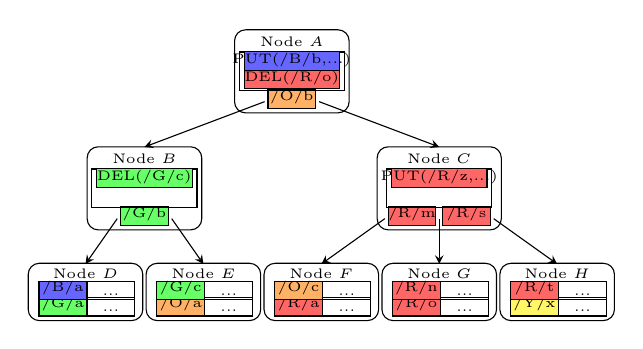
\begin{tikzpicture}[xscale=0.95, yscale=0.95]
        \node[anchor=south, rectangle, rounded corners, minimum height=.06\textwidth, minimum width=.12\textwidth, draw=black] at (0, 0) {};
        \node[anchor=south, font=\tiny] at (0, .036\textwidth) {Node $F$};
        \node[anchor=south, rectangle, minimum height=.015\textwidth, minimum width=.05\textwidth, draw=black, fill={red!60}] at (-.025\textwidth, .005\textwidth) {};
        \node[anchor=south, font=\tiny] at (-.025\textwidth, 0) {/R/a};
        \node[anchor=south, rectangle, minimum height=.015\textwidth, minimum width=.05\textwidth, draw=black] at (.028\textwidth, .005\textwidth) {};
        \node[anchor=south, font=\tiny] at (.028\textwidth, 0) {...};
        \node[anchor=south, rectangle, minimum height=.015\textwidth, minimum width=.05\textwidth, draw=black, fill={orange!60}] at (-.025\textwidth, .023\textwidth) {};
        \node[anchor=south, font=\tiny] at (-.025\textwidth, .018\textwidth) {/O/c};
        \node[anchor=south, rectangle, minimum height=.015\textwidth, minimum width=.05\textwidth, draw=black] at (.028\textwidth, .023\textwidth) {};
        \node[anchor=south, font=\tiny] at (.028\textwidth, .018\textwidth) {...};

        \node[anchor=south, rectangle, rounded corners, minimum height=.06\textwidth, minimum width=.12\textwidth, draw=black] at (.13\textwidth, 0) {};
        \node[anchor=south, font=\tiny] at (.13\textwidth, .036\textwidth) {Node $G$};
        \node[anchor=south, rectangle, minimum height=.015\textwidth, minimum width=.05\textwidth, draw=black, fill={red!60}] at (.105\textwidth, .005\textwidth) {};
        \node[anchor=south, font=\tiny] at (.105\textwidth, 0) {/R/o};
        \node[anchor=south, rectangle, minimum height=.015\textwidth, minimum width=.05\textwidth, draw=black] at (.158\textwidth, .005\textwidth) {};
        \node[anchor=south, font=\tiny] at (.158\textwidth, 0) {...};
        \node[anchor=south, rectangle, minimum height=.015\textwidth, minimum width=.05\textwidth, draw=black, fill={red!60}] at (.105\textwidth, .023\textwidth) {};
        \node[anchor=south, font=\tiny] at (.105\textwidth, .018\textwidth) {/R/n};
        \node[anchor=south, rectangle, minimum height=.015\textwidth, minimum width=.05\textwidth, draw=black] at (.158\textwidth, .023\textwidth) {};
        \node[anchor=south, font=\tiny] at (.158\textwidth, .018\textwidth) {...};

        \node[anchor=south, rectangle, rounded corners, minimum height=.06\textwidth, minimum width=.12\textwidth, draw=black] at (.26\textwidth, 0) {};
        \node[anchor=south, font=\tiny] at (.26\textwidth, .036\textwidth) {Node $H$};
        \node[anchor=south, rectangle, minimum height=.015\textwidth, minimum width=.05\textwidth, draw=black, fill={yellow!60}] at (.235\textwidth, .005\textwidth) {};
        \node[anchor=south, font=\tiny] at (.235\textwidth, 0) {/Y/x};
        \node[anchor=south, rectangle, minimum height=.015\textwidth, minimum width=.05\textwidth, draw=black] at (.288\textwidth, .005\textwidth) {};
        \node[anchor=south, font=\tiny] at (.288\textwidth, 0) {...};
        \node[anchor=south, rectangle, minimum height=.015\textwidth, minimum width=.05\textwidth, draw=black, fill={red!60}] at (.235\textwidth, .023\textwidth) {};
        \node[anchor=south, font=\tiny] at (.235\textwidth, .018\textwidth) {/R/t};
        \node[anchor=south, rectangle, minimum height=.015\textwidth, minimum width=.05\textwidth, draw=black] at (.288\textwidth, .023\textwidth) {};
        \node[anchor=south, font=\tiny] at (.288\textwidth, .018\textwidth) {...};

        \node[anchor=south, rectangle, rounded corners, minimum height=.06\textwidth, minimum width=.12\textwidth, draw=black] at (-.13\textwidth, 0) {};
        \node[anchor=south, font=\tiny] at (-.13\textwidth, .036\textwidth) {Node $E$};
        \node[anchor=south, rectangle, minimum height=.015\textwidth, minimum width=.05\textwidth, draw=black, fill={orange!60}] at (-.155\textwidth, .005\textwidth) {};
        \node[anchor=south, font=\tiny] at (-.155\textwidth, 0) {/O/a};
        \node[anchor=south, rectangle, minimum height=.015\textwidth, minimum width=.05\textwidth, draw=black] at (-.102\textwidth, .005\textwidth) {};
        \node[anchor=south, font=\tiny] at (-.102\textwidth, 0) {...};
        \node[anchor=south, rectangle, minimum height=.015\textwidth, minimum width=.05\textwidth, draw=black, fill={green!60}] at (-.155\textwidth, .023\textwidth) {};
        \node[anchor=south, font=\tiny] at (-.155\textwidth, .018\textwidth) {/G/c};
        \node[anchor=south, rectangle, minimum height=.015\textwidth, minimum width=.05\textwidth, draw=black] at (-.102\textwidth, .023\textwidth) {};
        \node[anchor=south, font=\tiny] at (-.102\textwidth, .018\textwidth) {...};

        \node[anchor=south, rectangle, rounded corners, minimum height=.06\textwidth, minimum width=.12\textwidth, draw=black] at (-.26\textwidth, 0) {};
        \node[anchor=south, font=\tiny] at (-.26\textwidth, .036\textwidth) {Node $D$};
        \node[anchor=south, rectangle, minimum height=.015\textwidth, minimum width=.05\textwidth, draw=black, fill={green!60}] at (-.285\textwidth, .005\textwidth) {};
        \node[anchor=south, font=\tiny] at (-.285\textwidth, 0) {/G/a};
        \node[anchor=south, rectangle, minimum height=.015\textwidth, minimum width=.05\textwidth, draw=black] at (-.232\textwidth, .005\textwidth) {};
        \node[anchor=south, font=\tiny] at (-.232\textwidth, 0) {...};
        \node[anchor=south, rectangle, minimum height=.015\textwidth, minimum width=.05\textwidth, draw=black, fill={blue!60}] at (-.285\textwidth, .023\textwidth) {};
        \node[anchor=south, font=\tiny] at (-.285\textwidth, .018\textwidth) {/B/a};
        \node[anchor=south, rectangle, minimum height=.015\textwidth, minimum width=.05\textwidth, draw=black] at (-.232\textwidth, .023\textwidth) {};
        \node[anchor=south, font=\tiny] at (-.232\textwidth, .018\textwidth) {...};

        \node[anchor=south, rectangle, rounded corners, minimum height=.087\textwidth, minimum width=.12\textwidth, draw=black] at (-.195\textwidth, .1\textwidth) {};
        \node[anchor=south, font=\tiny] at (-.195\textwidth, .163\textwidth) {Node $B$};
        \node[anchor=south, rectangle, minimum height=.015\textwidth, minimum width=.05\textwidth, draw=black, fill={green!60}] at (-.195\textwidth, .105\textwidth) {};
        \node[anchor=south, font=\tiny] at (-.195\textwidth, .1\textwidth) {/G/b};
        \node[anchor=south, rectangle, minimum height=.04\textwidth, minimum width=.11\textwidth, draw=black] at (-.195\textwidth, .125\textwidth) {};
        \node[anchor=south, rectangle, minimum height=.015\textwidth, minimum width=.1\textwidth, draw=black, fill={green!60}] at (-.195\textwidth, .147\textwidth) {};
        \node[anchor=south, font=\tiny] at  (-.195\textwidth, .141\textwidth) {DEL(/G/c)};

        \node[anchor=south, rectangle, rounded corners, minimum height=.087\textwidth, minimum width=.13\textwidth, draw=black] at (.13\textwidth, .1\textwidth) {};
        \node[anchor=south, font=\tiny] at (.13\textwidth, .163\textwidth) {Node $C$};
        \node[anchor=south, rectangle, minimum height=.015\textwidth, minimum width=.05\textwidth, draw=black, fill={red!60}] at (.1\textwidth, .105\textwidth) {};
        \node[anchor=south, font=\tiny] at (.1\textwidth, .1\textwidth) {/R/m};
        \node[anchor=south, rectangle, minimum height=.015\textwidth, minimum width=.05\textwidth, draw=black, fill={red!60}] at (.16\textwidth, .105\textwidth) {};
        \node[anchor=south, font=\tiny] at (.16\textwidth, .1\textwidth) {/R/s};
        \node[anchor=south, rectangle, minimum height=.04\textwidth, minimum width=.11\textwidth, draw=black] at (.13\textwidth, .125\textwidth) {};
        \node[anchor=south, rectangle, minimum height=.015\textwidth, minimum width=.1\textwidth, draw=black, fill={red!60}] at (.13\textwidth, .147\textwidth) {};
        \node[anchor=south, font=\tiny] at  (.13\textwidth, .141\textwidth) {PUT(/R/z,...)};

        \node[anchor=south, rectangle, rounded corners, minimum height=.087\textwidth, minimum width=.12\textwidth, draw=black] at (-.0325\textwidth, .229\textwidth) {};
        \node[anchor=south, font=\tiny] at (-.0325\textwidth, .292\textwidth) {Node $A$};
        \node[anchor=south, rectangle, minimum height=.015\textwidth, minimum width=.05\textwidth, draw=black, fill={orange!60}] at (-.0325\textwidth, .234\textwidth) {};
        \node[anchor=south, font=\tiny] at (-.0325\textwidth, .229\textwidth) {/O/b};
        \node[anchor=south, rectangle, minimum height=.04\textwidth, minimum width=.11\textwidth, draw=black] at (-.0325\textwidth, .254\textwidth) {};
        \node[anchor=south, rectangle, minimum height=.015\textwidth, minimum width=.1\textwidth, draw=black, fill={red!60}] at (-.0325\textwidth, .256\textwidth) {};
        \node[anchor=south, font=\tiny] at  (-.0325\textwidth, .25\textwidth) {DEL(/R/o)};
        \node[anchor=south, rectangle, minimum height=.015\textwidth, minimum width=.1\textwidth, draw=black, fill={blue!60}] at (-.0325\textwidth, .276\textwidth) {};
        \node[anchor=south, font=\tiny] at  (-.0325\textwidth, .27\textwidth) {PUT(/B/b,...)};

        \draw[->, >=stealth] (-.225\textwidth, .113\textwidth) -- (-.26\textwidth, .063\textwidth);
        \draw[->, >=stealth] (-.165\textwidth, .113\textwidth) -- (-.13\textwidth, .063\textwidth);
        \draw[->, >=stealth] (.13\textwidth, .113\textwidth) -- (.13\textwidth, .063\textwidth);
        \draw[->, >=stealth] (.19\textwidth, .113\textwidth) -- (.26\textwidth, .063\textwidth);
        \draw[->, >=stealth] (.07\textwidth, .113\textwidth) -- (0, .063\textwidth);
        \draw[->, >=stealth] (-.0625\textwidth, .242\textwidth) -- (-.195\textwidth, .192\textwidth);
        \draw[->, >=stealth] (-.0025\textwidth, .242\textwidth) -- (.13\textwidth, .192\textwidth);
    \end{tikzpicture}
    \caption[A \bet]{\label{fig:bet} A \bet.}
\end{figure}

\begin{table}[t]
    \centering
    \begin{tabular}{c | c c c}
        \hline
        Data Structure & Insert & Point Query & Range Query \\
        \hline
        \hline
        \btree & $O(log_{B}{N})$ & $O(log_{B}{N})$ & $O(log_{B}{N} + k/B)$\\
        \hline
        \bet & $O({log_{B}{N}}/{\varepsilon B^{1 - \varepsilon}})$ & $O({log_{B}{N}}/{\varepsilon})$ & $O({log_{B}{N}}/{\varepsilon} + k/B)$ \\
        \hline
        \bet ($\varepsilon=0.5$) & $O(log_{B}{N}/{\sqrt{B}})$ & $O(log_{B}{N})$ & $O(log_{B}{N} + k/B)$ \\
        \hline
    \end{tabular}
    \caption[The asymptotic IO costs of \btrees and \bets]{\label{tab:betbtree}
        The asymptotic IO costs of \btrees and \bets.}
\end{table}

\bets are asymptotically faster than \btrees, as summarized in
Table~\ref{tab:betbtree}.
Consider a \btree with $N$ key/value pairs and in which each node can hold
$B$ keys
(for simplicity, assume keys have constant size and that the value associated
with each key has negligible size).
The tree has fanout $B$, so its height is $O(log_{B}{N})$.
Inserts and point queries need to fetch all nodes along the root-to-leaf path,
resulting in $O(log_{B}{N})$ IOs.
A range query for $k$ key/value pairs requires $O(log_{B}{N} + k/B)$ IOs.

For comparison, a \bet with node size $B$ has fanout $B^{\varepsilon}$, where
$0 < \varepsilon \leq 1$.
Therefore, pivot keys in a non-leaf node consume $B^{\varepsilon}$ space and
the remaining $(B - B^{\varepsilon})$ space is used for buffers.
As a result, the \bet has height $O(log_{B}{N}/\varepsilon)$.
A point query fetches all nodes along the root-to-leaf path with
$O(log_{B}{N}/\varepsilon)$ IOs and a range query for $k$ key/value pairs
requires $O({log_{B}{N}}/{\varepsilon} + k/B)$ IOs.
On the other hand, the cost of an insert consists of injecting the message into
the root node with $O(1)$ IO and flushing the message down at each level.
In each flush, \bets has $O(B - B^{\varepsilon})$ messages and $B^{\varepsilon}$
children.
Thus, at leave one child can receive at least
$O((B - B^{\varepsilon})/B^{\varepsilon}) = O(B^{1 - \varepsilon})$ messages.
Therefore, the amortized cost of an insert in one flush is
$O(1/B^{1 - \varepsilon})$.
As the insert must be flushed $O(log_{B}{N}/\varepsilon)$ times, the amortized
cost of the insert is $O({log_{B}{N}}/{\varepsilon B^{1 - \varepsilon}})$.
A \bet with $\varepsilon = 1$ is equivalent to a \btree.
And if $\varepsilon = 1/2$, the point and range query costs of the \bet
become $O(log_{B}{N})$ and $O(log_{B}{N} + k/B)$, which is the same as a \btree,
but the insert cost becomes $O(log_{B}{N}/{\sqrt{B}})$, which is faster by a
factor of $\sqrt{B}$.

One important change in \bets from \btrees is the asymmetric IO costs for
point queries and inserts.
In \btrees, if an application wants to update the old value associated with a
key, it performs a point query to get the old value and then issues an insert
with the updated value.
Because both operations take $O(log_{B}{N})$ IOs, the total cost remains
$O(log_{B}{N})$.
However, in \bets, the query cost is $O(log_{B}{N}/\varepsilon)$ IOs while the
insert cost is $O({log_{B}{N}}/{\varepsilon B^{1 - \varepsilon}})$.
Performing a query before an insert degrades the total cost to
$O(log_{B}{N}/\varepsilon)$ IOs.

To avoid this read-before-write problem, \bets support ``upsert'' operations.
An upsert injects a message with the key and a delta into the buffer of the root
node.
When the upsert message is flushed to the leaf, it updates the old value
associated with the key with a user-specified function and the delta in the
message.
With upsert messages, queries need to compute value on the fly.
However, this doesn't change the IO costs of queries.
On the other hand, updating an old value becomes as fast as an insert.

\section{Full-path-indexed \betrfs}
\label{sec:fpi}

\begin{figure}[t]
    \centering
    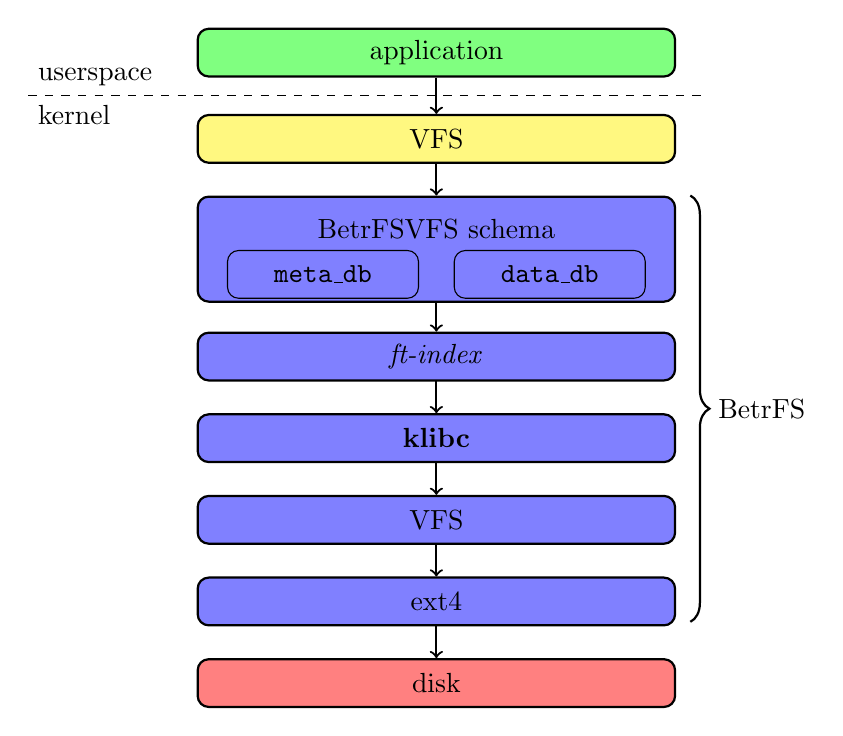
\begin{tikzpicture}[yscale=0.95, xscale=0.95]
    \draw[thick, ->] (0, .04\textwidth) -- (0, 0) node [anchor=north, rectangle, rounded corners, text centered, minimum height=.05\textwidth, minimum width=.5\textwidth, draw=black, fill=red!50] {disk};
    \draw[thick, ->] (0, .13\textwidth) -- (0, .09\textwidth) node [anchor=north, rectangle, rounded corners, text centered, minimum height=.05\textwidth, minimum width=.5\textwidth, draw=black, fill=blue!50] {ext4};
    \draw[thick, ->] (0, .22\textwidth) -- (0, .18\textwidth) node [anchor=north, rectangle, rounded corners, text centered, minimum height=.05\textwidth, minimum width=.5\textwidth, draw=black, fill=blue!50] {VFS};
    \draw[thick, ->] (0, .31\textwidth) -- (0, .27\textwidth) node [anchor=north, rectangle, rounded corners, text centered, minimum height=.05\textwidth, minimum width=.5\textwidth, draw=black, fill=blue!50] {\klibc};
    \draw[thick, ->] (0, .4\textwidth) -- (0, .36\textwidth) node [anchor=north, rectangle, rounded corners, text centered, minimum height=.05\textwidth, minimum width=.5\textwidth, draw=black, fill=blue!50] {\fti};
    \draw[thick, ->] (0, .55\textwidth) -- (0, .51\textwidth) node [anchor=north, rectangle, rounded corners, text centered, minimum height=.11\textwidth, minimum width=.5\textwidth, draw=black, fill=blue!50] {};
    \node [anchor=north, rectangle, rounded corners, text centered, minimum height=.05\textwidth, minimum width=.2\textwidth, draw=black, fill=blue!50] at (.125\textwidth, .45\textwidth) {\ddb};
    \node [anchor=north, rectangle, rounded corners, text centered, minimum height=.05\textwidth, minimum width=.2\textwidth, draw=black, fill=blue!50] at (-.125\textwidth, .45\textwidth) {\mdb};
    \node [anchor=north, text centered, minimum height=.05\textwidth] at (0, .50\textwidth) {\betrfs VFS schema};
    \draw[thick, ->] (0, .64\textwidth) -- (0, .60\textwidth) node [anchor=north, rectangle, rounded corners, text centered, minimum height=.05\textwidth, minimum width=.5\textwidth, draw=black, fill=yellow!50] {VFS};
    \node[anchor=south, rectangle, rounded corners, text centered, minimum height=.05\textwidth, minimum width=.5\textwidth, draw=black, thick, fill=green!50] at (0, .64\textwidth) {application};
    \draw[dashed] (-.45\textwidth, .62\textwidth) -- (.3\textwidth, .62\textwidth);
    \node[anchor=south west] at (-.45\textwidth, .62\textwidth) {userspace};
    \node[anchor=north west] at (-.45\textwidth, .62\textwidth) {kernel};
    \draw[decorate, decoration={brace,amplitude=.02\textwidth,mirror}, thick] (.28\textwidth, .04\textwidth) -- (.28\textwidth, .51\textwidth);
    \node[anchor=west,text centered] at (.3\textwidth, .275\textwidth) {\betrfs};
    \end{tikzpicture}
    \caption[The \betrfs architecture]{\label{fig:betrfs}
        The \betrfs architecture.}
\end{figure}

\betrfs~\citep{betrfs1,betrfs1tos} is a Linux in-kernel file
system built upon \fti~\citep{fti}, a key/value store that implements \bets and
exposes a key/value interface similar to BerkelyDB.
The architecture of \betrfs is shown in Figure~\ref{fig:betrfs}.
\betrfs interacts with \fti through point operations, such as \texttt{put},
\texttt{get} and \texttt{del}, as well as range queries with cursors
(\texttt{c\_get} with DB\_SET\_RANGE and DB\_NEXT).
\betrfs also uses the transaction interface of \fti to execute multiple
operations atomically.
A redo log and periodic checkpoints (every 60 seconds) in \fti ensure that
changes can be made persistent on disk.

\Fti cannot be integrated into a Linux kernel module easily because
it is a userspace library that assumes libc functions and system calls.
\betrfs has a shim layer called \klibc that implements all functions \fti
requires.
Through this way, \betrfs can incorporate \fti into the kernel module without
modifying code in \fti.

\betrfs uses two key/value indexes to store the metadata and data in the file
system.
One \mdb maps full-paths to \texttt{struct stat} structures.
Another \ddb maps (full-path and block number) to 4KB blocks.
When the VFS (Virtual File System) needs metadata, \betrfs queries
the \mdb with the full-path and constructs the corresponding inode
from the \texttt{struct stat}.
Likewise, when a dirty inode needs to be written, the \texttt{struct stat} is
assembled from the inode and written to the \mdb with the
full-path key.
Blocks of a file are fetched and written by the full-path and the indexes of
blocks.
Although other block granularity is possible, 4KB is the natural block size
because it is the same as the page size in the Linux page cache.

\betrfs can write to a block without fetching the old block to memory, avoiding
expensive read-before-write described in Section~\ref{sec:bet}.
Conventional file systems must read the old block from the disk to the page
cache before writing to that block (a complete overwrite can be done without
fetching the old block, but it is not implemented in any file system).
However, \bets have asymmetric read and write costs, so read-before-write should
be avoided.
In \betrfs, if the corresponding block is not in memory, an upsert message,
which describes the offset, length and content of this write, is injected into
the \bet.
When this message is flushed to the leaf, the change is applied to the old
block.

Full-path indexing ensures locality even with file system aging~\citep{betrfs3}.
After \betrfs fetches one block of a file from the disk, all nodes along the
root-to-leaf path are present in memory.
And with full-path indexing, all keys under one directory are contiguous in the
keyspace, which means a subsequent fetch of some other block in the same file or
another file under than same directory is likely to be resolved in memory,
which significantly increases performance and IO efficiency.

The first implementation of \betrfs (\betrfsOne) shows great random write
performance.
Recursive greps run 3.77x faster than in the best standard file system.
File creation runs 12.54x faster.
Small, random writes to a file run 68.24x faster~\citep{betrfs1tos}.

However, namespace operations have predictably miserable performance in
\betrfsOne.
Deleting and renaming a Linux source directory takes 46.14 and 21.17 seconds,
respectively, because the file system has to call one or more key/value store
operations for each key.
The deleting problem is fixed by a range-delete message that nullifies all
messages within a range, but the renaming problem remains difficult.

\section{Relative-path-indexed \betrfs}
\label{sec:rpi}

\begin{figure}[t]
    \begin{subfigure}{.5\textwidth}
        \centering
        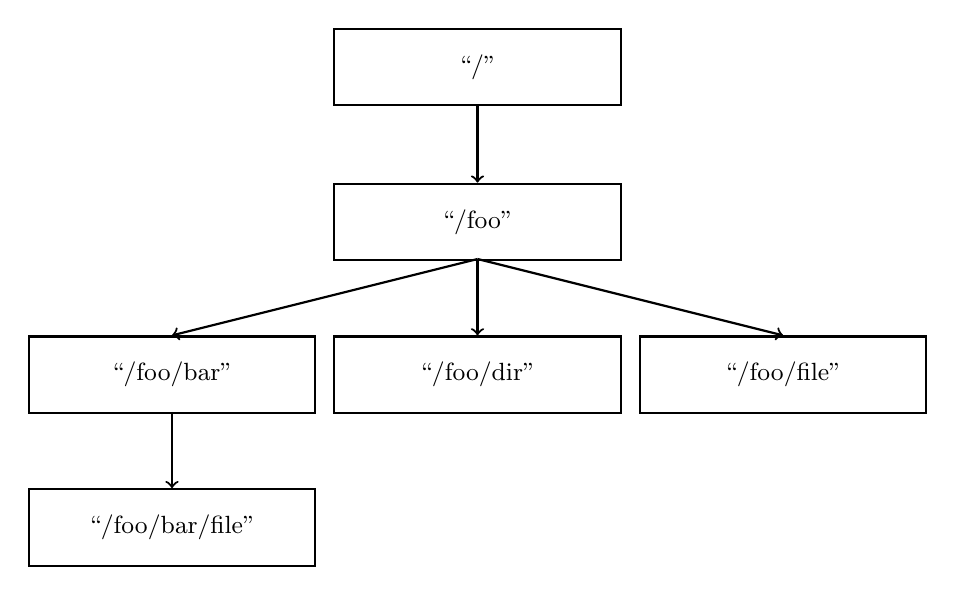
\begin{tikzpicture}{xscale=0.95,yscale=0.95}
            \draw[thick, ->] (0, .08\textwidth) -- (0, 0) node [anchor=north, rectangle, text centered, minimum height=.08\textwidth, minimum width=.3\textwidth, draw=black, font=\small] {``/foo/bar/file''};
            \draw[thick, ->] (.32\textwidth, .24\textwidth) -- (0, .16\textwidth) node [anchor=north, rectangle, text centered, minimum height=.08\textwidth, minimum width=.3\textwidth, draw=black, font=\small] {``/foo/bar''};
            \draw[thick, ->] (.32\textwidth, .24\textwidth) -- (.32\textwidth, .16\textwidth) node [anchor=north, rectangle, text centered, minimum height=.08\textwidth, minimum width=.3\textwidth, draw=black, font=\small] {``/foo/dir''};
            \draw[thick, ->] (.32\textwidth, .24\textwidth) -- (.64\textwidth, .16\textwidth) node [anchor=north, rectangle, text centered, minimum height=.08\textwidth, minimum width=.3\textwidth, draw=black, font=\small] {``/foo/file''};
            \draw[thick, ->] (.32\textwidth, .4\textwidth) -- (.32\textwidth, .32\textwidth) node [anchor=north, rectangle, text centered, minimum height=.08\textwidth, minimum width=.3\textwidth, draw=black, font=\small] {``/foo''};
            \node [anchor=south, rectangle, text centered, minimum height=.08\textwidth, minimum width=.3\textwidth, draw=black, thick, font=\small] at (.32\textwidth, .4\textwidth) {``/''};
        \end{tikzpicture}
        \caption{\label{subfig:FPI} Full-path indexing.}
    \end{subfigure}
    \begin{subfigure}{.5\textwidth}
        \centering
        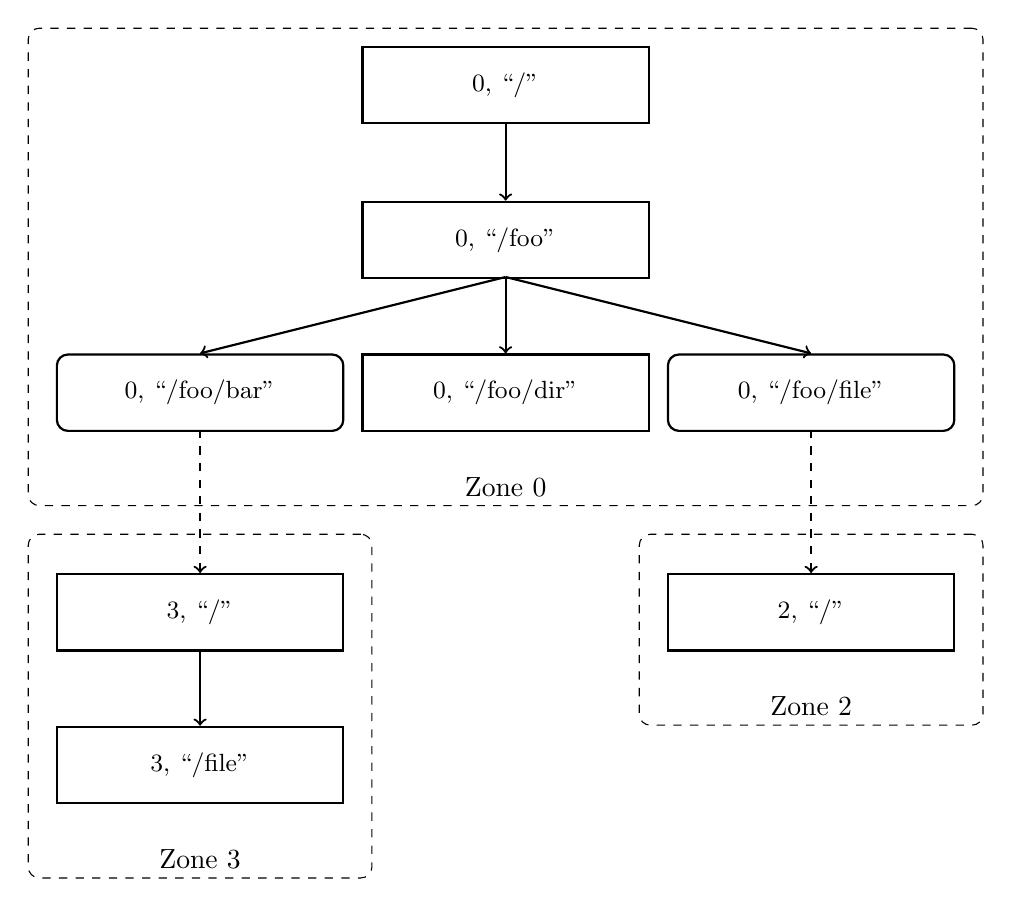
\begin{tikzpicture}{xscale=0.95,yscale=0.95}
            \node [anchor=south, rectangle, rounded corners, minimum height=.50\textwidth, minimum width=\textwidth, draw=black, dashed] at (.32\textwidth, 0) {};
            \node [anchor=south] at (.32\textwidth, 0) {Zone 0};
            \draw[thick, ->] (.32\textwidth, .24\textwidth) -- (0, .16\textwidth) node [anchor=north, rectangle, rounded corners, text centered, minimum height=.08\textwidth, minimum width=.3\textwidth, draw=black, font=\small] {0, ``/foo/bar''};
            \draw[thick, ->] (.32\textwidth, .24\textwidth) -- (.32\textwidth, .16\textwidth) node [anchor=north, rectangle, text centered, minimum height=.08\textwidth, minimum width=.3\textwidth, draw=black, font=\small] {0, ``/foo/dir''};
            \draw[thick, ->] (.32\textwidth, .24\textwidth) -- (.64\textwidth, .16\textwidth) node [anchor=north, rectangle, rounded corners, text centered, minimum height=.08\textwidth, minimum width=.3\textwidth, draw=black, font=\small] {0, ``/foo/file''};
            \draw[thick, ->] (.32\textwidth, .4\textwidth) -- (.32\textwidth, .32\textwidth) node [anchor=north, rectangle, text centered, minimum height=.08\textwidth, minimum width=.3\textwidth, draw=black, font=\small] {0, ``/foo''};
            \node [anchor=south, rectangle, text centered, minimum height=.08\textwidth, minimum width=.3\textwidth, draw=black, thick, font=\small] at (.32\textwidth, .4\textwidth) {0, ``/''};
            \node [anchor=south, rectangle, rounded corners, minimum height=.36\textwidth, minimum width=.36\textwidth, draw=black, dashed] at (0, -.39\textwidth) {};
            \node [anchor=south] at (0, -.39\textwidth) {Zone 3};
            \node [anchor=north, rectangle, text centered, minimum height=.08\textwidth, minimum width=.3\textwidth, draw=black, thick, font=\small] at (0, -.07\textwidth) {3, ``/''};
            \draw[thick, ->] (0, -.15\textwidth) -- (0, -.23\textwidth) node [anchor=north, rectangle, text centered, minimum height=.08\textwidth, minimum width=.3\textwidth, draw=black, font=\small] {3, ``/file''};
            \node [anchor=south, rectangle, rounded corners, minimum height=.2\textwidth, minimum width=.36\textwidth, draw=black, dashed] at (.64\textwidth, -.23\textwidth) {};
            \node [anchor=south] at (.64\textwidth, -.23\textwidth) {Zone 2};
            \node [anchor=north, rectangle, text centered, minimum height=.08\textwidth, minimum width=.3\textwidth, draw=black, thick, font=\small] at (.64\textwidth, -.07\textwidth) {2, ``/''};
            \draw[thick, dashed, ->] (0, .08\textwidth) -- (0, -.07\textwidth);
            \draw[thick, dashed, ->] (.64\textwidth, .08\textwidth) -- (.64\textwidth, -.07\textwidth);
        \end{tikzpicture}
        \caption{\label{subfig:RPI} Relative-path indexing.}
    \end{subfigure}
    \caption[Full-path indexing and relative-path indexing]{\label{fig:FPIRPI}
        Full-path indexing and relative-path indexing.}
\end{figure}

Relative-path-indexed \betrfs~\citep{betrfs2,betrfs2tos} backed away from
full-path indexing and introduced relative-path indexing,
which is also called zoning.
Relative-path indexing partitions the directory hierarchy into zones.
Each zone has a zone ID (the root zone has zone ID 0), which is analogous to an
inode number, and a single root file or directory.
All file or directory in a zone is indexed relative to the zone root.
If the file or directory is the root of another zone, the entry contains that
zone ID to redirect queries.

Figure~\ref{fig:FPIRPI} shows an example of the same directory hierarchy under
full-path indexing and relative-path indexing.
In Figure~\ref{subfig:RPI}, when querying the key/value store for file
``/foo/file'' with key (0, ``/foo/file''), the file system gets a special value
indicating it is the root of Zone 2.
Subsequently, the file system queries the key/value store with key (2, ``/'')
and gets the right value.
Similary, the file system notices the key for directory ``/foo/bar'' is
(3, ``/'').
Therefore, when querying for file ``/foo/bar/file'', it uses key (3, ``/file'').

\newcommand{\addTokubenchZonePlot}[1]
{
    \addplot[
        color=\pgfkeysvalueof{/fs-colors/#1},
        line width=0.75pt,
        mark=\pgfkeysvalueof{/fs-marks/#1},
    ]
    plot[
    ]
    table[
    ]
    {./data/tokuzone/#1.csv};
    \addlegendentry{\pgfkeysvalueof{/fs-names/#1}}
}

\begin{figure}[t]
    \centering
    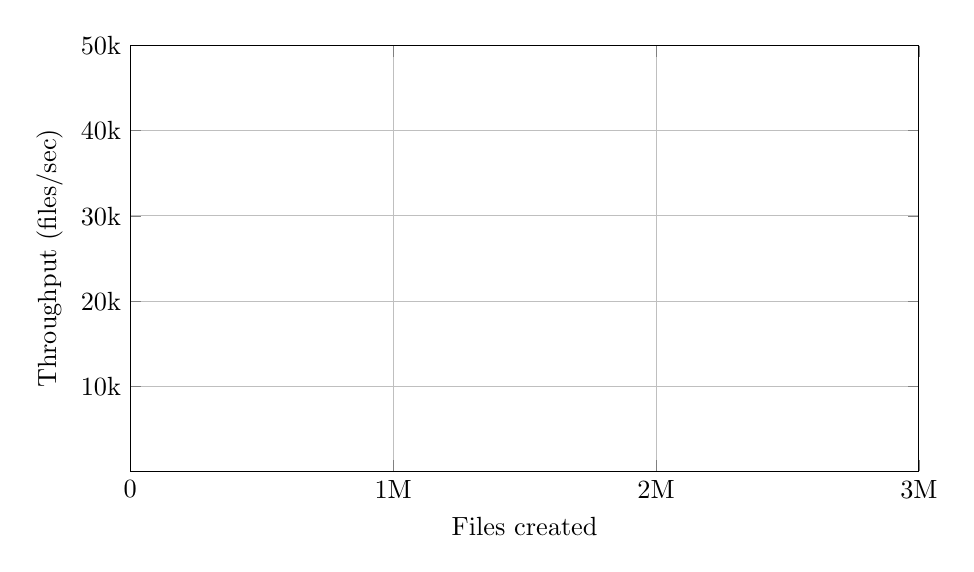
\begin{tikzpicture}[yscale=0.95,xscale=0.95]
        \begin{axis}[
            xlabel={Files created},
            ylabel={Throughput (files/sec)},
            xmin=0,
            xmax=3000000,
            ymin=10,
            ymax=50000,
            mark repeat=10,
            xtick={0,1000000,2000000,3000000},
            xticklabels={0,1M,2M,3M},
            ytick={10000,20000,30000,40000,50000},
            yticklabels={10k,20k,30k,40k,50k},
            grid=major,
            scaled x ticks=false,
            scaled y ticks=false,
            legend cell align=left,
            transpose legend,
            height=.6\linewidth,
            width=\linewidth,
        ]
        \addTokubenchZonePlot{betrfs3};
        \addTokubenchZonePlot{betrfs3-max};
        \end{axis}
    \end{tikzpicture}
    \caption[Zone maintainance cost in TokuBench benchmark]{Cumulative file creation
        throughput during the Tokubench benchmark (higher is better).
        Compared to \betrfsThree with one zone, \betrfsThree has a sudden
        performance drop because of zone splitting.}
    \label{fig:tokuzone}
\end{figure}

Relative-path indexing tries to balance locality and rename performance through
a target zone size.
Larger zone size means better locality because full-path indexing is still
maintained within the zone.
Smaller zone size imposes a lower bound on rename latency
because no rename needs to mutate more key/value pairs than in a zone.

\betrfsTwo adopts relative-path-indexing with a default zone size 128KiB.
Relative-path indexing made renames on \betrfsTwo almost as fast as inode-based
file system and recursive-directory traversals almost as fast as \betrfsOne.

However, relative-path indexing also imposes zone maintenance costs on other
file system operations.
For instance, in Figure~\ref{fig:tokuzone},
two-thirds of the way through the TokuBench benchmark,
\betrfsThree (\betrfsThree is \betrfsTwo with some bug fixes) shows a sudden,
precipitous drop in cumulative throughput for small file creation,
because the file system performs a huge amount of zone splitting.
On the contrary, \betrfsThree with an infinite zone size (marked as \betrfsThree
with one zone) has a smooth curve throughout the benchmark.

Furthermore, relative-path indexing also has bad worst-case performance.
It is possible to construct arrangements of nested directories that will each
reside in their own zone.
Reading a file in the deepest directory will require reading one zone per
directory (each withits own I/O).
Such a pathological worst case is not possible with full-path indexing in a
\bet, and an important design goal for \betrfs is keeping a reasonable bound on
the worst cases.

\section{Summary}

\betrfs is a general file system designed for all operations, with a particular
focus on random writes and locality.
The underlying data structure, \bets, performs random writes faster than \btrees
by cascading writes in batches.
The full-path indexing schema of \betrfsOne ensures good locality, while making
renames slow.
The relative-path indexing schema of \betrfsTwo enables fast renames,
but imposes additional costs on other operations.



\chapter{Range-Rename}
\label{chap:rename}

This chapter describes the range-rename operation~\citep{betrfs4,betrfs4tos}
on \bets.
Full-path-indexed \betrfs can implement a file system rename by invoking the
range-rename operation on the \bet that updates all related key in the rename.
For example, renaming ``/foo'' to ``/bar'' invokes a range-rename operation
that updates all keys with prefix ``/foo'' to have prefix ``/bar''.
The goal of this design is to get good locality from full-path indexing
while having good rename performance through an efficient range-rename
implementation.

Section~\ref{sec:rr:int} describes the range-rename interface and shows how
\betrfs can implement file system renames by calling range-rename operations.
Then, Section~\ref{sec:rr:op} discusses how to implement the range-rename operation
in an I/O-efficient way on \bets.
In particular, the range-rename operation introduces two key techniques,
\textbf{tree surgery} (Section~\ref{sec:rr:op:surgery}) and
\textbf{key lifting} (Section~\ref{sec:rr:op:lift}).
Finally, Section~\ref{sec:rr:impl} explains implementation details of
the range-rename operation in \fti and \betrfs.

\section{The range-rename interface}
\label{sec:rr:int}

Range-rename is a new key/value store operation defined as
range-rename(\spre, \dpre).
The range-rename operation takes two prefixes, \spre and \dpre, as arguments
and updates source and destination key/value pairs
(a source/destination key/value pair has the prefix \spre/\dpre in its key).
Range-rename(\spre, \dpre) does three things atomically:
\begin{itemize}
\item the range-rename operation deletes all destination key/value pairs
    from the key/value store
\item then, for each source key/value pair $(k,v)$ in the key/value store,
    the range-rename operation inserts a key/value pair $(k',v)$
    to the key/value store, where $k$ is the concatenation of \spre and some
    suffix $s$ and $k'$ is the concatenation of \dpre and the same suffix $s$;
\item at last, the range-rename operation deletes all source key/value pairs
    from the key/value store.
\end{itemize}
In other words, the range-rename deletes all destination key/value pairs and
updates all source key/value pairs, changing the key prefix from \spre to \dpre.

To see how range-rename accomplishes file system renames in full-path-indexed
\betrfs, consider renaming file ``/foo'' to ``/bar''.
In \mdb, \betrfs needs to insert the destination key ``/bar''
(this insert overwrites the old value of ``/bar'', if it exists)
and delete the source key ``/foo'', resulting in two operations on the \bet.
On the other hand, in \ddb, \betrfs needs to delete all data keys of ``/bar''
(POSIX allows file renames to overwrite the destination file) and update all
data keys of ``/foo'' to be data keys of ``/bar''.
The whole work in \ddb can be done by calling range-rename(``/foo'',``/bar'')
(a data key is the concatenation of the full-path and an 8-byte block number).

Similarly, consider renaming directory ``/baz'' to ``/qux''.
In \mdb, \betrfs also needs to insert the destination key ``/qux'' and delete
the source key ``/baz'' with two operations on the \bet.
Additionally, \betrfs needs to update all keys with prefix ``/baz/'' to have
prefix ``/qux/''
(POSIX only allows directory renames to overwrite an empty directory, which
means there cannot be any key with prefix ``/qux/''),
which is handled in range-rename(``/baz/'', ``/qux/'').
Likewise, in \ddb, \betrfs needs to update all keys with prefix ``/baz/''
to have prefix ``/qux/'', which is done by range-rename(``/baz/'', ``/qux/'')
(directory doesn't have any data key).

Also, \betrfs puts all operations in a file system rename in a transaction
so that all changes are committed atomically.

\begin{table}[t]
    \centering
    \begin{tabular}{c | l}
        \hline
        Type of Rename & Key/Value Store Operations \\
        \hline
        \hline
        File Rename & transaction\_begin(); \\
                    & \mdb$\rightarrow$put(\textit{dst}); \\
                    & \mdb$\rightarrow$del(\textit{src}); \\
                    & \ddb$\rightarrow$range-rename(\textit{src}, \textit{dst}); \\
                    & transaction\_end(); \\
        \hline
        Directory Rename & transaction\_begin(); \\
                         & \mdb$\rightarrow$put(\textit{dst}); \\
                         & \mdb$\rightarrow$del(\textit{src}); \\
                         & \mdb$\rightarrow$range-rename(\textit{src/}, \textit{dst/}); \\
                         & \ddb$\rightarrow$range-rename(\textit{src/}, \textit{dst/}); \\
                         & transaction\_end(); \\
        \hline
    \end{tabular}
    \caption[Full-path-indexed \betrfs implements file system renames with range-rename]{\label{tab:fsrr}
        Full-path-indexed \betrfs renames \textit{src} to \textit{dst} by
        invoking range-rename and other operations on \bets in a transaction.}
\end{table}

Table~\ref{tab:fsrr} summarizes how file system renames can be done with
range-rename operations in full-path-index \betrfs.
Briefly speaking, full-path-indexed \betrfs can finish a file rename by
invoking three operations on \bets: an insert, a delete and a range-rename
operation.
And a directory rename can be done with an insert, a delete and two
range-rename operations.

In fact, previous full-path-indexed \betrfs implemented the
range-rename operation with existing \bet operations,
\texttt{del}, \texttt{get} and \texttt{put}.
However, this range-rename implementation updates all source and destination
key/value pairs.
The I/O-cost of this range-rename implementation increases
when the number of source and destination key/value pairs grows.
Efficient file system renames in full-path-indexed \betrfs require an efficient
range-rename implementation, that is, a range-rename implementation that
completes in a bounded number of I/Os
that doesn't grow as the number of related keys grows.

\section{The range-rename operation}
\label{sec:rr:op}

This section describes the range-rename implementation on the
\bet whose cost doesn't grow as the number of related keys grows.
The efficient range-rename operation requires lexicographic key order so that
keys with the same prefix are contiguous in the key space.
With contiguous keys, the range-rename operation can create an isolated subtree,
which contains all keys of a certain prefix in the \bet,
through \textbf{tree surgery}.
Then, the range-rename operation moves the isolated subtree to another location
in the \bet.
The prefixes of keys in the subtree are updated automatically through
\textbf{key lifting}, which transforms \bets into lifted \bets.

Section~\ref{sec:rr:op:surgery} describes tree surgery, which splits nodes in the
\bet to create an isolated subtree of a prefix.
Tree surgery also flushes messages in the \bet to push all related messages into
the isolated subtree.
Then, Section~\ref{sec:rr:op:lift} introduces key lifting, which transforms the
\bets into lifted \bets that update prefixes of keys in a subtree
automatically when the subtree is moved to another location.
At last, Section~\ref{sec:rr:op:rr} combines the two techniques and shows how
to implement the efficient range-rename operation on lifted \bets.

\subsection{Tree surgery}
\label{sec:rr:op:surgery}

\begin{figure}
    \begin{subfigure}{\textwidth}
        \centering
        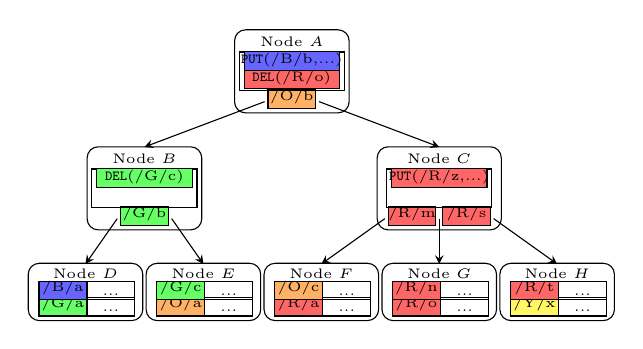
\begin{tikzpicture}[xscale=0.95, yscale=0.95]
            \node[anchor=south, rectangle, rounded corners, minimum height=.06\textwidth, minimum width=.12\textwidth, draw=black] at (0, 0) {};
            \node[anchor=south, font=\tiny] at (0, .036\textwidth) {Node $F$};
            \node[anchor=south, rectangle, minimum height=.015\textwidth, minimum width=.05\textwidth, draw=black, fill={red!60}] at (-.025\textwidth, .005\textwidth) {};
            \node[anchor=south, font=\tiny] at (-.025\textwidth, 0) {/R/a};
            \node[anchor=south, rectangle, minimum height=.015\textwidth, minimum width=.05\textwidth, draw=black] at (.028\textwidth, .005\textwidth) {};
            \node[anchor=south, font=\tiny] at (.028\textwidth, 0) {...};
            \node[anchor=south, rectangle, minimum height=.015\textwidth, minimum width=.05\textwidth, draw=black, fill={orange!60}] at (-.025\textwidth, .023\textwidth) {};
            \node[anchor=south, font=\tiny] at (-.025\textwidth, .018\textwidth) {/O/c};
            \node[anchor=south, rectangle, minimum height=.015\textwidth, minimum width=.05\textwidth, draw=black] at (.028\textwidth, .023\textwidth) {};
            \node[anchor=south, font=\tiny] at (.028\textwidth, .018\textwidth) {...};

            \node[anchor=south, rectangle, rounded corners, minimum height=.06\textwidth, minimum width=.12\textwidth, draw=black] at (.13\textwidth, 0) {};
            \node[anchor=south, font=\tiny] at (.13\textwidth, .036\textwidth) {Node $G$};
            \node[anchor=south, rectangle, minimum height=.015\textwidth, minimum width=.05\textwidth, draw=black, fill={red!60}] at (.105\textwidth, .005\textwidth) {};
            \node[anchor=south, font=\tiny] at (.105\textwidth, 0) {/R/o};
            \node[anchor=south, rectangle, minimum height=.015\textwidth, minimum width=.05\textwidth, draw=black] at (.158\textwidth, .005\textwidth) {};
            \node[anchor=south, font=\tiny] at (.158\textwidth, 0) {...};
            \node[anchor=south, rectangle, minimum height=.015\textwidth, minimum width=.05\textwidth, draw=black, fill={red!60}] at (.105\textwidth, .023\textwidth) {};
            \node[anchor=south, font=\tiny] at (.105\textwidth, .018\textwidth) {/R/n};
            \node[anchor=south, rectangle, minimum height=.015\textwidth, minimum width=.05\textwidth, draw=black] at (.158\textwidth, .023\textwidth) {};
            \node[anchor=south, font=\tiny] at (.158\textwidth, .018\textwidth) {...};

            \node[anchor=south, rectangle, rounded corners, minimum height=.06\textwidth, minimum width=.12\textwidth, draw=black] at (.26\textwidth, 0) {};
            \node[anchor=south, font=\tiny] at (.26\textwidth, .036\textwidth) {Node $H$};
            \node[anchor=south, rectangle, minimum height=.015\textwidth, minimum width=.05\textwidth, draw=black, fill={yellow!60}] at (.235\textwidth, .005\textwidth) {};
            \node[anchor=south, font=\tiny] at (.235\textwidth, 0) {/Y/x};
            \node[anchor=south, rectangle, minimum height=.015\textwidth, minimum width=.05\textwidth, draw=black] at (.288\textwidth, .005\textwidth) {};
            \node[anchor=south, font=\tiny] at (.288\textwidth, 0) {...};
            \node[anchor=south, rectangle, minimum height=.015\textwidth, minimum width=.05\textwidth, draw=black, fill={red!60}] at (.235\textwidth, .023\textwidth) {};
            \node[anchor=south, font=\tiny] at (.235\textwidth, .018\textwidth) {/R/t};
            \node[anchor=south, rectangle, minimum height=.015\textwidth, minimum width=.05\textwidth, draw=black] at (.288\textwidth, .023\textwidth) {};
            \node[anchor=south, font=\tiny] at (.288\textwidth, .018\textwidth) {...};

            \node[anchor=south, rectangle, rounded corners, minimum height=.06\textwidth, minimum width=.12\textwidth, draw=black] at (-.13\textwidth, 0) {};
            \node[anchor=south, font=\tiny] at (-.13\textwidth, .036\textwidth) {Node $E$};
            \node[anchor=south, rectangle, minimum height=.015\textwidth, minimum width=.05\textwidth, draw=black, fill={orange!60}] at (-.155\textwidth, .005\textwidth) {};
            \node[anchor=south, font=\tiny] at (-.155\textwidth, 0) {/O/a};
            \node[anchor=south, rectangle, minimum height=.015\textwidth, minimum width=.05\textwidth, draw=black] at (-.102\textwidth, .005\textwidth) {};
            \node[anchor=south, font=\tiny] at (-.102\textwidth, 0) {...};
            \node[anchor=south, rectangle, minimum height=.015\textwidth, minimum width=.05\textwidth, draw=black, fill={green!60}] at (-.155\textwidth, .023\textwidth) {};
            \node[anchor=south, font=\tiny] at (-.155\textwidth, .018\textwidth) {/G/c};
            \node[anchor=south, rectangle, minimum height=.015\textwidth, minimum width=.05\textwidth, draw=black] at (-.102\textwidth, .023\textwidth) {};
            \node[anchor=south, font=\tiny] at (-.102\textwidth, .018\textwidth) {...};

            \node[anchor=south, rectangle, rounded corners, minimum height=.06\textwidth, minimum width=.12\textwidth, draw=black] at (-.26\textwidth, 0) {};
            \node[anchor=south, font=\tiny] at (-.26\textwidth, .036\textwidth) {Node $D$};
            \node[anchor=south, rectangle, minimum height=.015\textwidth, minimum width=.05\textwidth, draw=black, fill={green!60}] at (-.285\textwidth, .005\textwidth) {};
            \node[anchor=south, font=\tiny] at (-.285\textwidth, 0) {/G/a};
            \node[anchor=south, rectangle, minimum height=.015\textwidth, minimum width=.05\textwidth, draw=black] at (-.232\textwidth, .005\textwidth) {};
            \node[anchor=south, font=\tiny] at (-.232\textwidth, 0) {...};
            \node[anchor=south, rectangle, minimum height=.015\textwidth, minimum width=.05\textwidth, draw=black, fill={blue!60}] at (-.285\textwidth, .023\textwidth) {};
            \node[anchor=south, font=\tiny] at (-.285\textwidth, .018\textwidth) {/B/a};
            \node[anchor=south, rectangle, minimum height=.015\textwidth, minimum width=.05\textwidth, draw=black] at (-.232\textwidth, .023\textwidth) {};
            \node[anchor=south, font=\tiny] at (-.232\textwidth, .018\textwidth) {...};

            \node[anchor=south, rectangle, rounded corners, minimum height=.087\textwidth, minimum width=.12\textwidth, draw=black] at (-.195\textwidth, .1\textwidth) {};
            \node[anchor=south, font=\tiny] at (-.195\textwidth, .163\textwidth) {Node $B$};
            \node[anchor=south, rectangle, minimum height=.015\textwidth, minimum width=.05\textwidth, draw=black, fill={green!60}] at (-.195\textwidth, .105\textwidth) {};
            \node[anchor=south, font=\tiny] at (-.195\textwidth, .1\textwidth) {/G/b};
            \node[anchor=south, rectangle, minimum height=.04\textwidth, minimum width=.11\textwidth, draw=black] at (-.195\textwidth, .125\textwidth) {};
            \node[anchor=south, rectangle, minimum height=.015\textwidth, minimum width=.1\textwidth, draw=black, fill={green!60}] at (-.195\textwidth, .147\textwidth) {};
            \node[anchor=south, font=\tiny] at  (-.195\textwidth, .141\textwidth) {\delm(/G/c)};

            \node[anchor=south, rectangle, rounded corners, minimum height=.087\textwidth, minimum width=.13\textwidth, draw=black] at (.13\textwidth, .1\textwidth) {};
            \node[anchor=south, font=\tiny] at (.13\textwidth, .163\textwidth) {Node $C$};
            \node[anchor=south, rectangle, minimum height=.015\textwidth, minimum width=.05\textwidth, draw=black, fill={red!60}] at (.1\textwidth, .105\textwidth) {};
            \node[anchor=south, font=\tiny] at (.1\textwidth, .1\textwidth) {/R/m};
            \node[anchor=south, rectangle, minimum height=.015\textwidth, minimum width=.05\textwidth, draw=black, fill={red!60}] at (.16\textwidth, .105\textwidth) {};
            \node[anchor=south, font=\tiny] at (.16\textwidth, .1\textwidth) {/R/s};
            \node[anchor=south, rectangle, minimum height=.04\textwidth, minimum width=.11\textwidth, draw=black] at (.13\textwidth, .125\textwidth) {};
            \node[anchor=south, rectangle, minimum height=.015\textwidth, minimum width=.1\textwidth, draw=black, fill={red!60}] at (.13\textwidth, .147\textwidth) {};
            \node[anchor=south, font=\tiny] at  (.13\textwidth, .141\textwidth) {\putm(/R/z,...)};

            \node[anchor=south, rectangle, rounded corners, minimum height=.087\textwidth, minimum width=.12\textwidth, draw=black] at (-.0325\textwidth, .229\textwidth) {};
            \node[anchor=south, font=\tiny] at (-.0325\textwidth, .292\textwidth) {Node $A$};
            \node[anchor=south, rectangle, minimum height=.015\textwidth, minimum width=.05\textwidth, draw=black, fill={orange!60}] at (-.0325\textwidth, .234\textwidth) {};
            \node[anchor=south, font=\tiny] at (-.0325\textwidth, .229\textwidth) {/O/b};
            \node[anchor=south, rectangle, minimum height=.04\textwidth, minimum width=.11\textwidth, draw=black] at (-.0325\textwidth, .254\textwidth) {};
            \node[anchor=south, rectangle, minimum height=.015\textwidth, minimum width=.1\textwidth, draw=black, fill={red!60}] at (-.0325\textwidth, .256\textwidth) {};
            \node[anchor=south, font=\tiny] at  (-.0325\textwidth, .25\textwidth) {\delm(/R/o)};
            \node[anchor=south, rectangle, minimum height=.015\textwidth, minimum width=.1\textwidth, draw=black, fill={blue!60}] at (-.0325\textwidth, .276\textwidth) {};
            \node[anchor=south, font=\tiny] at  (-.0325\textwidth, .27\textwidth) {\putm(/B/b,...)};

            \draw[->, >=stealth] (-.225\textwidth, .113\textwidth) -- (-.26\textwidth, .063\textwidth);
            \draw[->, >=stealth] (-.165\textwidth, .113\textwidth) -- (-.13\textwidth, .063\textwidth);
            \draw[->, >=stealth] (.13\textwidth, .113\textwidth) -- (.13\textwidth, .063\textwidth);
            \draw[->, >=stealth] (.19\textwidth, .113\textwidth) -- (.26\textwidth, .063\textwidth);
            \draw[->, >=stealth] (.07\textwidth, .113\textwidth) -- (0, .063\textwidth);
            \draw[->, >=stealth] (-.0625\textwidth, .242\textwidth) -- (-.195\textwidth, .192\textwidth);
            \draw[->, >=stealth] (-.0025\textwidth, .242\textwidth) -- (.13\textwidth, .192\textwidth);
        \end{tikzpicture}
        \caption{\label{subfig:slice-1} The \bet before tree surgery.}
    \end{subfigure}
    \begin{subfigure}{\textwidth}
        \centering
        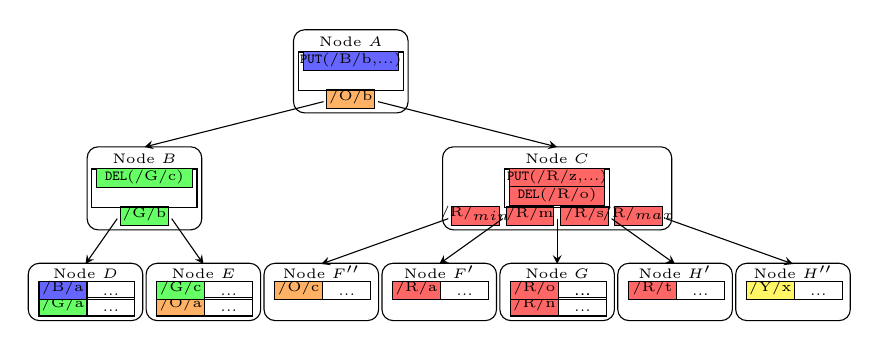
\begin{tikzpicture}[xscale=0.95, yscale=0.95]
            \node[anchor=south, rectangle, rounded corners, minimum height=.06\textwidth, minimum width=.12\textwidth, draw=black] at (0, 0) {};
            \node[anchor=south, font=\tiny] at (0, .036\textwidth) {Node $F''$};
            \node[anchor=south, rectangle, minimum height=.015\textwidth, minimum width=.05\textwidth, draw=black, fill={orange!60}] at (-.025\textwidth, .023\textwidth) {};
            \node[anchor=south, font=\tiny] at (-.025\textwidth, .018\textwidth) {/O/c};
            \node[anchor=south, rectangle, minimum height=.015\textwidth, minimum width=.05\textwidth, draw=black] at (.028\textwidth, .023\textwidth) {};
            \node[anchor=south, font=\tiny] at (.028\textwidth, .018\textwidth) {...};

            \node[anchor=south, rectangle, rounded corners, minimum height=.06\textwidth, minimum width=.12\textwidth, draw=black] at (.13\textwidth, 0) {};
            \node[anchor=south, font=\tiny] at (.13\textwidth, .036\textwidth) {Node $F'$};
            \node[anchor=south, rectangle, minimum height=.015\textwidth, minimum width=.05\textwidth, draw=black, fill={red!60}] at (.105\textwidth, .023\textwidth) {};
            \node[anchor=south, font=\tiny] at (.105\textwidth, .018\textwidth) {/R/a};
            \node[anchor=south, rectangle, minimum height=.015\textwidth, minimum width=.05\textwidth, draw=black] at (.158\textwidth, .023\textwidth) {};
            \node[anchor=south, font=\tiny] at (.158\textwidth, .018\textwidth) {...};

            \node[anchor=south, rectangle, rounded corners, minimum height=.06\textwidth, minimum width=.12\textwidth, draw=black] at (.26\textwidth, 0) {};
            \node[anchor=south, font=\tiny] at (.26\textwidth, .036\textwidth) {Node $G$};
            \node[anchor=south, rectangle, minimum height=.015\textwidth, minimum width=.05\textwidth, draw=black, fill={red!60}] at (.235\textwidth, .005\textwidth) {};
            \node[anchor=south, font=\tiny] at (.235\textwidth, 0) {/R/n};
            \node[anchor=south, rectangle, minimum height=.015\textwidth, minimum width=.05\textwidth, draw=black] at (.288\textwidth, .005\textwidth) {};
            \node[anchor=south, font=\tiny] at (.288\textwidth, 0) {...};
            \node[anchor=south, rectangle, minimum height=.015\textwidth, minimum width=.05\textwidth, draw=black, fill={red!60}] at (.235\textwidth, .023\textwidth) {};
            \node[anchor=south, font=\tiny] at (.235\textwidth, .018\textwidth) {/R/o};
            \node[anchor=south, rectangle, minimum height=.015\textwidth, minimum width=.05\textwidth, draw=black] at (.288\textwidth, .023\textwidth) {};
            \node[anchor=south, font=\tiny] at (.288\textwidth, .018\textwidth) {...};

            \node[anchor=south, rectangle, rounded corners, minimum height=.06\textwidth, minimum width=.12\textwidth, draw=black] at (.39\textwidth, 0) {};
            \node[anchor=south, font=\tiny] at (.39\textwidth, .036\textwidth) {Node $H'$};
            \node[anchor=south, rectangle, minimum height=.015\textwidth, minimum width=.05\textwidth, draw=black, fill={red!60}] at (.365\textwidth, .023\textwidth) {};
            \node[anchor=south, font=\tiny] at (.365\textwidth, .018\textwidth) {/R/t};
            \node[anchor=south, rectangle, minimum height=.015\textwidth, minimum width=.05\textwidth, draw=black] at (.418\textwidth, .023\textwidth) {};
            \node[anchor=south, font=\tiny] at (.418\textwidth, .018\textwidth) {...};

            \node[anchor=south, rectangle, rounded corners, minimum height=.06\textwidth, minimum width=.12\textwidth, draw=black] at (.52\textwidth, 0) {};
            \node[anchor=south, font=\tiny] at (.52\textwidth, .036\textwidth) {Node $H''$};
            \node[anchor=south, rectangle, minimum height=.015\textwidth, minimum width=.05\textwidth, draw=black, fill={yellow!60}] at (.495\textwidth, .023\textwidth) {};
            \node[anchor=south, font=\tiny] at (.495\textwidth, .018\textwidth) {/Y/x};
            \node[anchor=south, rectangle, minimum height=.015\textwidth, minimum width=.05\textwidth, draw=black] at (.548\textwidth, .023\textwidth) {};
            \node[anchor=south, font=\tiny] at (.548\textwidth, .018\textwidth) {...};

            \node[anchor=south, rectangle, minimum height=.015\textwidth, minimum width=.05\textwidth, draw=black] at (.288\textwidth, .023\textwidth) {};
            \node[anchor=south, font=\tiny] at (.288\textwidth, .018\textwidth) {...};
            \node[anchor=south, rectangle, rounded corners, minimum height=.06\textwidth, minimum width=.12\textwidth, draw=black] at (-.13\textwidth, 0) {};
            \node[anchor=south, font=\tiny] at (-.13\textwidth, .036\textwidth) {Node $E$};
            \node[anchor=south, rectangle, minimum height=.015\textwidth, minimum width=.05\textwidth, draw=black, fill={orange!60}] at (-.155\textwidth, .005\textwidth) {};
            \node[anchor=south, font=\tiny] at (-.155\textwidth, 0) {/O/a};
            \node[anchor=south, rectangle, minimum height=.015\textwidth, minimum width=.05\textwidth, draw=black] at (-.102\textwidth, .005\textwidth) {};
            \node[anchor=south, font=\tiny] at (-.102\textwidth, 0) {...};
            \node[anchor=south, rectangle, minimum height=.015\textwidth, minimum width=.05\textwidth, draw=black, fill={green!60}] at (-.155\textwidth, .023\textwidth) {};
            \node[anchor=south, font=\tiny] at (-.155\textwidth, .018\textwidth) {/G/c};
            \node[anchor=south, rectangle, minimum height=.015\textwidth, minimum width=.05\textwidth, draw=black] at (-.102\textwidth, .023\textwidth) {};
            \node[anchor=south, font=\tiny] at (-.102\textwidth, .018\textwidth) {...};

            \node[anchor=south, rectangle, rounded corners, minimum height=.06\textwidth, minimum width=.12\textwidth, draw=black] at (-.26\textwidth, 0) {};
            \node[anchor=south, font=\tiny] at (-.26\textwidth, .036\textwidth) {Node $D$};
            \node[anchor=south, rectangle, minimum height=.015\textwidth, minimum width=.05\textwidth, draw=black, fill={green!60}] at (-.285\textwidth, .005\textwidth) {};
            \node[anchor=south, font=\tiny] at (-.285\textwidth, 0) {/G/a};
            \node[anchor=south, rectangle, minimum height=.015\textwidth, minimum width=.05\textwidth, draw=black] at (-.232\textwidth, .005\textwidth) {};
            \node[anchor=south, font=\tiny] at (-.232\textwidth, 0) {...};
            \node[anchor=south, rectangle, minimum height=.015\textwidth, minimum width=.05\textwidth, draw=black, fill={blue!60}] at (-.285\textwidth, .023\textwidth) {};
            \node[anchor=south, font=\tiny] at (-.285\textwidth, .018\textwidth) {/B/a};
            \node[anchor=south, rectangle, minimum height=.015\textwidth, minimum width=.05\textwidth, draw=black] at (-.232\textwidth, .023\textwidth) {};
            \node[anchor=south, font=\tiny] at (-.232\textwidth, .018\textwidth) {...};

            \node[anchor=south, rectangle, rounded corners, minimum height=.087\textwidth, minimum width=.12\textwidth, draw=black] at (-.195\textwidth, .1\textwidth) {};
            \node[anchor=south, font=\tiny] at (-.195\textwidth, .163\textwidth) {Node $B$};
            \node[anchor=south, rectangle, minimum height=.015\textwidth, minimum width=.05\textwidth, draw=black, fill={green!60}] at (-.195\textwidth, .105\textwidth) {};
            \node[anchor=south, font=\tiny] at (-.195\textwidth, .1\textwidth) {/G/b};
            \node[anchor=south, rectangle, minimum height=.04\textwidth, minimum width=.11\textwidth, draw=black] at (-.195\textwidth, .125\textwidth) {};
            \node[anchor=south, rectangle, minimum height=.015\textwidth, minimum width=.1\textwidth, draw=black, fill={green!60}] at (-.195\textwidth, .147\textwidth) {};
            \node[anchor=south, font=\tiny] at  (-.195\textwidth, .141\textwidth) {\delm(/G/c)};

            \node[anchor=south, rectangle, rounded corners, minimum height=.087\textwidth, minimum width=.24\textwidth, draw=black] at (.26\textwidth, .1\textwidth) {};
            \node[anchor=south, font=\tiny] at (.26\textwidth, .163\textwidth) {Node $C$};
            \node[anchor=south, rectangle, minimum height=.015\textwidth, minimum width=.05\textwidth, draw=black, fill={red!60}] at (.17\textwidth, .105\textwidth) {};
            \node[anchor=south, font=\tiny] at (.17\textwidth, .1\textwidth) {/R/$_{min}$};
            \node[anchor=south, rectangle, minimum height=.015\textwidth, minimum width=.05\textwidth, draw=black, fill={red!60}] at (.23\textwidth, .105\textwidth) {};
            \node[anchor=south, font=\tiny] at (.23\textwidth, .1\textwidth) {/R/m};
            \node[anchor=south, rectangle, minimum height=.015\textwidth, minimum width=.05\textwidth, draw=black, fill={red!60}] at (.29\textwidth, .105\textwidth) {};
            \node[anchor=south, font=\tiny] at (.29\textwidth, .1\textwidth) {/R/s};
            \node[anchor=south, rectangle, minimum height=.015\textwidth, minimum width=.05\textwidth, draw=black, fill={red!60}] at (.35\textwidth, .105\textwidth) {};
            \node[anchor=south, font=\tiny] at (.35\textwidth, .1\textwidth) {/R/$_{max}$};
            \node[anchor=south, rectangle, minimum height=.04\textwidth, minimum width=.11\textwidth, draw=black] at (.26\textwidth, .125\textwidth) {};
            \node[anchor=south, rectangle, minimum height=.015\textwidth, minimum width=.1\textwidth, draw=black, fill={red!60}] at (.26\textwidth, .147\textwidth) {};
            \node[anchor=south, font=\tiny] at  (.26\textwidth, .141\textwidth) {\putm(/R/z,...)};
            \node[anchor=south, rectangle, minimum height=.015\textwidth, minimum width=.1\textwidth, draw=black, fill={red!60}] at (.26\textwidth, .127\textwidth) {};
            \node[anchor=south, font=\tiny] at  (.26\textwidth, .121\textwidth) {\delm(/R/o)};

            \node[anchor=south, rectangle, rounded corners, minimum height=.087\textwidth, minimum width=.12\textwidth, draw=black] at (.0325\textwidth, .229\textwidth) {};
            \node[anchor=south, font=\tiny] at (.0325\textwidth, .292\textwidth) {Node $A$};
            \node[anchor=south, rectangle, minimum height=.015\textwidth, minimum width=.05\textwidth, draw=black, fill={orange!60}] at (.0325\textwidth, .234\textwidth) {};
            \node[anchor=south, font=\tiny] at (.0325\textwidth, .229\textwidth) {/O/b};
            \node[anchor=south, rectangle, minimum height=.04\textwidth, minimum width=.11\textwidth, draw=black] at (.0325\textwidth, .254\textwidth) {};
            \node[anchor=south, rectangle, minimum height=.015\textwidth, minimum width=.1\textwidth, draw=black, fill={blue!60}] at (.0325\textwidth, .276\textwidth) {};
            \node[anchor=south, font=\tiny] at  (.0325\textwidth, .27\textwidth) {\putm(/B/b,...)};

            \draw[->, >=stealth] (-.225\textwidth, .113\textwidth) -- (-.26\textwidth, .063\textwidth);
            \draw[->, >=stealth] (-.165\textwidth, .113\textwidth) -- (-.13\textwidth, .063\textwidth);
            \draw[->, >=stealth] (.26\textwidth, .113\textwidth) -- (.26\textwidth, .063\textwidth);
            \draw[->, >=stealth] (.32\textwidth, .113\textwidth) -- (.39\textwidth, .063\textwidth);
            \draw[->, >=stealth] (.38\textwidth, .113\textwidth) -- (.52\textwidth, .063\textwidth);
            \draw[->, >=stealth] (.20\textwidth, .113\textwidth) -- (.13\textwidth, .063\textwidth);
            \draw[->, >=stealth] (.14\textwidth, .113\textwidth) -- (0, .063\textwidth);
            \draw[->, >=stealth] (.0025\textwidth, .242\textwidth) -- (-.195\textwidth, .192\textwidth);
            \draw[->, >=stealth] (.0625\textwidth, .242\textwidth) -- (.26\textwidth, .192\textwidth);
        \end{tikzpicture}
        \caption{\label{subfig:slice-2} Tree surgery splits leaf nodes.}
    \end{subfigure}
    \begin{subfigure}{\textwidth}
        \centering
        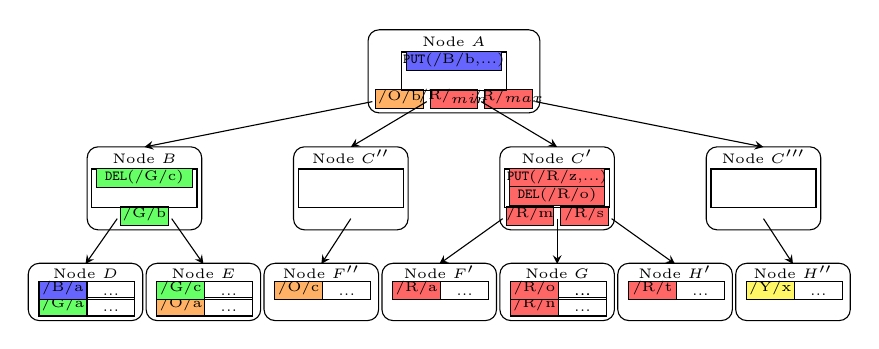
\begin{tikzpicture}[xscale=0.95, yscale=0.95]
            \node[anchor=south, rectangle, rounded corners, minimum height=.06\textwidth, minimum width=.12\textwidth, draw=black] at (0, 0) {};
            \node[anchor=south, font=\tiny] at (0, .036\textwidth) {Node $F''$};
            \node[anchor=south, rectangle, minimum height=.015\textwidth, minimum width=.05\textwidth, draw=black, fill={orange!60}] at (-.025\textwidth, .023\textwidth) {};
            \node[anchor=south, font=\tiny] at (-.025\textwidth, .018\textwidth) {/O/c};
            \node[anchor=south, rectangle, minimum height=.015\textwidth, minimum width=.05\textwidth, draw=black] at (.028\textwidth, .023\textwidth) {};
            \node[anchor=south, font=\tiny] at (.028\textwidth, .018\textwidth) {...};

            \node[anchor=south, rectangle, rounded corners, minimum height=.06\textwidth, minimum width=.12\textwidth, draw=black] at (.13\textwidth, 0) {};
            \node[anchor=south, font=\tiny] at (.13\textwidth, .036\textwidth) {Node $F'$};
            \node[anchor=south, rectangle, minimum height=.015\textwidth, minimum width=.05\textwidth, draw=black, fill={red!60}] at (.105\textwidth, .023\textwidth) {};
            \node[anchor=south, font=\tiny] at (.105\textwidth, .018\textwidth) {/R/a};
            \node[anchor=south, rectangle, minimum height=.015\textwidth, minimum width=.05\textwidth, draw=black] at (.158\textwidth, .023\textwidth) {};
            \node[anchor=south, font=\tiny] at (.158\textwidth, .018\textwidth) {...};

            \node[anchor=south, rectangle, rounded corners, minimum height=.06\textwidth, minimum width=.12\textwidth, draw=black] at (.26\textwidth, 0) {};
            \node[anchor=south, font=\tiny] at (.26\textwidth, .036\textwidth) {Node $G$};
            \node[anchor=south, rectangle, minimum height=.015\textwidth, minimum width=.05\textwidth, draw=black, fill={red!60}] at (.235\textwidth, .005\textwidth) {};
            \node[anchor=south, font=\tiny] at (.235\textwidth, 0) {/R/n};
            \node[anchor=south, rectangle, minimum height=.015\textwidth, minimum width=.05\textwidth, draw=black] at (.288\textwidth, .005\textwidth) {};
            \node[anchor=south, font=\tiny] at (.288\textwidth, 0) {...};
            \node[anchor=south, rectangle, minimum height=.015\textwidth, minimum width=.05\textwidth, draw=black, fill={red!60}] at (.235\textwidth, .023\textwidth) {};
            \node[anchor=south, font=\tiny] at (.235\textwidth, .018\textwidth) {/R/o};
            \node[anchor=south, rectangle, minimum height=.015\textwidth, minimum width=.05\textwidth, draw=black] at (.288\textwidth, .023\textwidth) {};
            \node[anchor=south, font=\tiny] at (.288\textwidth, .018\textwidth) {...};

            \node[anchor=south, rectangle, rounded corners, minimum height=.06\textwidth, minimum width=.12\textwidth, draw=black] at (.39\textwidth, 0) {};
            \node[anchor=south, font=\tiny] at (.39\textwidth, .036\textwidth) {Node $H'$};
            \node[anchor=south, rectangle, minimum height=.015\textwidth, minimum width=.05\textwidth, draw=black, fill={red!60}] at (.365\textwidth, .023\textwidth) {};
            \node[anchor=south, font=\tiny] at (.365\textwidth, .018\textwidth) {/R/t};
            \node[anchor=south, rectangle, minimum height=.015\textwidth, minimum width=.05\textwidth, draw=black] at (.418\textwidth, .023\textwidth) {};
            \node[anchor=south, font=\tiny] at (.418\textwidth, .018\textwidth) {...};

            \node[anchor=south, rectangle, rounded corners, minimum height=.06\textwidth, minimum width=.12\textwidth, draw=black] at (.52\textwidth, 0) {};
            \node[anchor=south, font=\tiny] at (.52\textwidth, .036\textwidth) {Node $H''$};
            \node[anchor=south, rectangle, minimum height=.015\textwidth, minimum width=.05\textwidth, draw=black, fill={yellow!60}] at (.495\textwidth, .023\textwidth) {};
            \node[anchor=south, font=\tiny] at (.495\textwidth, .018\textwidth) {/Y/x};
            \node[anchor=south, rectangle, minimum height=.015\textwidth, minimum width=.05\textwidth, draw=black] at (.548\textwidth, .023\textwidth) {};
            \node[anchor=south, font=\tiny] at (.548\textwidth, .018\textwidth) {...};

            \node[anchor=south, rectangle, minimum height=.015\textwidth, minimum width=.05\textwidth, draw=black] at (.288\textwidth, .023\textwidth) {};
            \node[anchor=south, font=\tiny] at (.288\textwidth, .018\textwidth) {...};
            \node[anchor=south, rectangle, rounded corners, minimum height=.06\textwidth, minimum width=.12\textwidth, draw=black] at (-.13\textwidth, 0) {};
            \node[anchor=south, font=\tiny] at (-.13\textwidth, .036\textwidth) {Node $E$};
            \node[anchor=south, rectangle, minimum height=.015\textwidth, minimum width=.05\textwidth, draw=black, fill={orange!60}] at (-.155\textwidth, .005\textwidth) {};
            \node[anchor=south, font=\tiny] at (-.155\textwidth, 0) {/O/a};
            \node[anchor=south, rectangle, minimum height=.015\textwidth, minimum width=.05\textwidth, draw=black] at (-.102\textwidth, .005\textwidth) {};
            \node[anchor=south, font=\tiny] at (-.102\textwidth, 0) {...};
            \node[anchor=south, rectangle, minimum height=.015\textwidth, minimum width=.05\textwidth, draw=black, fill={green!60}] at (-.155\textwidth, .023\textwidth) {};
            \node[anchor=south, font=\tiny] at (-.155\textwidth, .018\textwidth) {/G/c};
            \node[anchor=south, rectangle, minimum height=.015\textwidth, minimum width=.05\textwidth, draw=black] at (-.102\textwidth, .023\textwidth) {};
            \node[anchor=south, font=\tiny] at (-.102\textwidth, .018\textwidth) {...};

            \node[anchor=south, rectangle, rounded corners, minimum height=.06\textwidth, minimum width=.12\textwidth, draw=black] at (-.26\textwidth, 0) {};
            \node[anchor=south, font=\tiny] at (-.26\textwidth, .036\textwidth) {Node $D$};
            \node[anchor=south, rectangle, minimum height=.015\textwidth, minimum width=.05\textwidth, draw=black, fill={green!60}] at (-.285\textwidth, .005\textwidth) {};
            \node[anchor=south, font=\tiny] at (-.285\textwidth, 0) {/G/a};
            \node[anchor=south, rectangle, minimum height=.015\textwidth, minimum width=.05\textwidth, draw=black] at (-.232\textwidth, .005\textwidth) {};
            \node[anchor=south, font=\tiny] at (-.232\textwidth, 0) {...};
            \node[anchor=south, rectangle, minimum height=.015\textwidth, minimum width=.05\textwidth, draw=black, fill={blue!60}] at (-.285\textwidth, .023\textwidth) {};
            \node[anchor=south, font=\tiny] at (-.285\textwidth, .018\textwidth) {/B/a};
            \node[anchor=south, rectangle, minimum height=.015\textwidth, minimum width=.05\textwidth, draw=black] at (-.232\textwidth, .023\textwidth) {};
            \node[anchor=south, font=\tiny] at (-.232\textwidth, .018\textwidth) {...};

            \node[anchor=south, rectangle, rounded corners, minimum height=.087\textwidth, minimum width=.12\textwidth, draw=black] at (-.195\textwidth, .1\textwidth) {};
            \node[anchor=south, font=\tiny] at (-.195\textwidth, .163\textwidth) {Node $B$};
            \node[anchor=south, rectangle, minimum height=.015\textwidth, minimum width=.05\textwidth, draw=black, fill={green!60}] at (-.195\textwidth, .105\textwidth) {};
            \node[anchor=south, font=\tiny] at (-.195\textwidth, .1\textwidth) {/G/b};
            \node[anchor=south, rectangle, minimum height=.04\textwidth, minimum width=.11\textwidth, draw=black] at (-.195\textwidth, .125\textwidth) {};
            \node[anchor=south, rectangle, minimum height=.015\textwidth, minimum width=.1\textwidth, draw=black, fill={green!60}] at (-.195\textwidth, .147\textwidth) {};
            \node[anchor=south, font=\tiny] at  (-.195\textwidth, .141\textwidth) {\delm(/G/c)};

            \node[anchor=south, rectangle, rounded corners, minimum height=.087\textwidth, minimum width=.12\textwidth, draw=black] at (.0325\textwidth, .1\textwidth) {};
            \node[anchor=south, font=\tiny] at (.0325\textwidth, .163\textwidth) {Node $C''$};
            \node[anchor=south, rectangle, minimum height=.04\textwidth, minimum width=.11\textwidth, draw=black] at (.0325\textwidth, .125\textwidth) {};

            \node[anchor=south, rectangle, rounded corners, minimum height=.087\textwidth, minimum width=.12\textwidth, draw=black] at (.26\textwidth, .1\textwidth) {};
            \node[anchor=south, font=\tiny] at (.26\textwidth, .163\textwidth) {Node $C'$};
            \node[anchor=south, rectangle, minimum height=.015\textwidth, minimum width=.05\textwidth, draw=black, fill={red!60}] at (.23\textwidth, .105\textwidth) {};
            \node[anchor=south, font=\tiny] at (.23\textwidth, .1\textwidth) {/R/m};
            \node[anchor=south, rectangle, minimum height=.015\textwidth, minimum width=.05\textwidth, draw=black, fill={red!60}] at (.29\textwidth, .105\textwidth) {};
            \node[anchor=south, font=\tiny] at (.29\textwidth, .1\textwidth) {/R/s};
            \node[anchor=south, rectangle, minimum height=.04\textwidth, minimum width=.11\textwidth, draw=black] at (.26\textwidth, .125\textwidth) {};
            \node[anchor=south, rectangle, minimum height=.015\textwidth, minimum width=.1\textwidth, draw=black, fill={red!60}] at (.26\textwidth, .147\textwidth) {};
            \node[anchor=south, font=\tiny] at  (.26\textwidth, .141\textwidth) {\putm(/R/z,...)};
            \node[anchor=south, rectangle, minimum height=.015\textwidth, minimum width=.1\textwidth, draw=black, fill={red!60}] at (.26\textwidth, .127\textwidth) {};
            \node[anchor=south, font=\tiny] at  (.26\textwidth, .121\textwidth) {\delm(/R/o)};

            \node[anchor=south, rectangle, rounded corners, minimum height=.087\textwidth, minimum width=.12\textwidth, draw=black] at (.4875\textwidth, .1\textwidth) {};
            \node[anchor=south, font=\tiny] at (.4875\textwidth, .163\textwidth) {Node $C'''$};
            \node[anchor=south, rectangle, minimum height=.04\textwidth, minimum width=.11\textwidth, draw=black] at (.4875\textwidth, .125\textwidth) {};

            \node[anchor=south, rectangle, rounded corners, minimum height=.087\textwidth, minimum width=.18\textwidth, draw=black] at (.14625\textwidth, .229\textwidth) {};
            \node[anchor=south, font=\tiny] at (.14625\textwidth, .292\textwidth) {Node $A$};
            \node[anchor=south, rectangle, minimum height=.015\textwidth, minimum width=.05\textwidth, draw=black, fill={orange!60}] at (.08625\textwidth, .234\textwidth) {};
            \node[anchor=south, font=\tiny] at (.08625\textwidth, .229\textwidth) {/O/b};
            \node[anchor=south, rectangle, minimum height=.015\textwidth, minimum width=.05\textwidth, draw=black, fill={red!60}] at (.14625\textwidth, .234\textwidth) {};
            \node[anchor=south, font=\tiny] at (.14625\textwidth, .229\textwidth) {/R/$_{min}$};
            \node[anchor=south, rectangle, minimum height=.015\textwidth, minimum width=.05\textwidth, draw=black, fill={red!60}] at (.20625\textwidth, .234\textwidth) {};
            \node[anchor=south, font=\tiny] at (.20625\textwidth, .229\textwidth) {/R/$_{max}$};
            \node[anchor=south, rectangle, minimum height=.04\textwidth, minimum width=.11\textwidth, draw=black] at (.14625\textwidth, .254\textwidth) {};
            \node[anchor=south, rectangle, minimum height=.015\textwidth, minimum width=.1\textwidth, draw=black, fill={blue!60}] at (.14625\textwidth, .276\textwidth) {};
            \node[anchor=south, font=\tiny] at  (.14625\textwidth, .27\textwidth) {\putm(/B/b,...)};

            \draw[->, >=stealth] (-.225\textwidth, .113\textwidth) -- (-.26\textwidth, .063\textwidth);
            \draw[->, >=stealth] (-.165\textwidth, .113\textwidth) -- (-.13\textwidth, .063\textwidth);
            \draw[->, >=stealth] (.26\textwidth, .113\textwidth) -- (.26\textwidth, .063\textwidth);
            \draw[->, >=stealth] (.32\textwidth, .113\textwidth) -- (.39\textwidth, .063\textwidth);
            \draw[->, >=stealth] (.4875\textwidth, .113\textwidth) -- (.52\textwidth, .063\textwidth);
            \draw[->, >=stealth] (.20\textwidth, .113\textwidth) -- (.13\textwidth, .063\textwidth);
            \draw[->, >=stealth] (.0325\textwidth, .113\textwidth) -- (0, .063\textwidth);
            \draw[->, >=stealth] (.05625\textwidth, .242\textwidth) -- (-.195\textwidth, .192\textwidth);
            \draw[->, >=stealth] (.11625\textwidth, .242\textwidth) -- (.0325\textwidth, .192\textwidth);
            \draw[->, >=stealth] (.17625\textwidth, .242\textwidth) -- (.26\textwidth, .192\textwidth);
            \draw[->, >=stealth] (.23625\textwidth, .242\textwidth) -- (.4875\textwidth, .192\textwidth);
        \end{tikzpicture}
        \caption{\label{subfig:slice-3} Tree surgery splits the LCA.}
    \end{subfigure}
    \caption[A tree surgery example]{\label{fig:slice}
        Tree surgery slices out an isolated subtree of prefix ``/R/''.}
\end{figure}

The goal of tree surgery is to slice out an isolated subtree of a certain
prefix $p$ in the \bet.
In the \bet, each node covers a certain key range, bounded by the key range and
pivots of its parent.
For a certain key range $(p_{min}, p_{max})$ ($p_{min}$ and $p_{max}$ are the
minimum and maximum keys with prefix $p$, respectively), there are three types
of nodes in the \bet:
nodes whose key ranges are completely out of the key range (exterior nodes),
nodes whose key ranges are completely in the key range (interior nodes),
and nodes whose key ranges partly overlap with the key range (fringe nodes).

In the \bet shown in Figure~\ref{subfig:slice-1},
consider prefix ``/R/'' with key range (``/R/$_{min}$'', ``/R/$_{min}$''),
Node $B$, $D$ and $E$ are exterior nodes, Node $G$ is an interior node,
and the other nodes are fringe nodes.

\paragraph{Identifying fringe nodes.}
The first step of tree surgery is to identify all fringe nodes.
Because the key range of a fringe node partly overlaps with key range
$(p_{min}, p_{max})$,
a fringe node must include either $p_{min}$ or $p_{max}$ in its key range.
Therefore, tree surgery can perform two root-to-leaf traversals with two keys,
$p_{min}$ and $p_{max}$, to identify all fringe nodes.
For example, in Figure~\ref{subfig:slice-1}, we walk down the \bet with
``/R/$_{min}$'' and ``/R/$_{max}$'' to identify all fringe nodes of
prefix ``/R/'',
Node $A$, $C$, $F$ and $H$.

An important fringe node for tree surgery is the \textbf{LCA}
(Lowest Common Ancestor) of the two traversing keys, that is, the lowest
(the most distant from the root node)
\bet node whose key range includes both keys.
For example, in Figure~\ref{subfig:slice-1}, Node $C$ is the LCA of prefix
``/R/''.
The subtree rooted at the LCA is the lowest subtree in the \bet that covers
the whole range $(p_{min}, p_{max})$.
The goal of tree surgery is to generate an isolated subtree rooted at the LCA
that contains all keys with prefix $p$.
Therefore, before reaching the LCA, the traversals also flush messages from
the parent to the child so that there is no pending message above the LCA.

\paragraph{Slicing.}
The goal of slicing is to separate unrelated keys in the fringe nodes
from keys in the key range (thus with prefix $p$).
With all related messages and key/value pairs in the subtree rooted at the LCA,
tree surgery starts slicing out the isolated subtree
by splitting fringe nodes from the bottom up.
Slicing uses the same code as standard \bet node splits, but,
rather than picking a key in the middle of the node,
divides the node at one of the slicing keys, $p_{min}$ or $p_{max}$.

Figure~\ref{subfig:slice-2} shows the \bet after the bottom-up slicing splits
leaf nodes.
Tree surgery splits Node $F$ with key ``/R/$_{min}$'', generating an interior
node, Node $F'$, and an exterior node, Node $F''$.
Likewise, tree surgery splits Node $H$ into an interior node, Node $H'$, and
an exterior node, Node $H'$, with key ``/R/$_{max}$''.
Note, the message \delm(``/R/o'') has been flushed from Node $A$ to Node $C$
before slicing.

At last, in Figure~\ref{subfig:slice-3}, tree surgery splits the LCA, Node $C$,
into Node $C'$, $C''$ and $C'''$ with both keys, ``/R/$_{min}$'' and
``/R/$_{max}$''.
The subtree rooted at Node $C'$ is the isolated subtree that contains and
only contains all keys with the prefix ``/R/''.

A special case in tree surgery is when the LCA is the root node of the \bet.
In such a scenario, splitting the root node divides the tree into a forest.
To avoid such case, we create a new root node as the parent of the old root
node before slicing.

\subsection{Key lifting}
\label{sec:rr:op:lift}

\begin{figure}
    \begin{subfigure}{\textwidth}
        \centering
        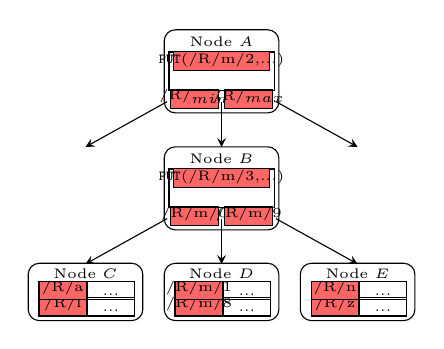
\begin{tikzpicture}[xscale=0.95, yscale=0.95]
            \node[anchor=south, rectangle, rounded corners, minimum height=.06\textwidth, minimum width=.12\textwidth, draw=black] at (0, 0) {};
            \node[anchor=south, font=\tiny] at (0, .036\textwidth) {Node $D$};
            \node[anchor=south, rectangle, minimum height=.015\textwidth, minimum width=.05\textwidth, draw=black, fill={red!60}] at (-.025\textwidth, .005\textwidth) {};
            \node[anchor=south, font=\tiny] at (-.025\textwidth, 0) {/R/m/8};
            \node[anchor=south, rectangle, minimum height=.015\textwidth, minimum width=.05\textwidth, draw=black] at (.028\textwidth, .005\textwidth) {};
            \node[anchor=south, font=\tiny] at (.028\textwidth, 0) {...};
            \node[anchor=south, rectangle, minimum height=.015\textwidth, minimum width=.05\textwidth, draw=black, fill={red!60}] at (-.025\textwidth, .023\textwidth) {};
            \node[anchor=south, font=\tiny] at (-.025\textwidth, .018\textwidth) {/R/m/1};
            \node[anchor=south, rectangle, minimum height=.015\textwidth, minimum width=.05\textwidth, draw=black] at (.028\textwidth, .023\textwidth) {};
            \node[anchor=south, font=\tiny] at (.028\textwidth, .018\textwidth) {...};

            \node[anchor=south, rectangle, rounded corners, minimum height=.06\textwidth, minimum width=.12\textwidth, draw=black] at (.15\textwidth, 0) {};
            \node[anchor=south, font=\tiny] at (.15\textwidth, .036\textwidth) {Node $E$};
            \node[anchor=south, rectangle, minimum height=.015\textwidth, minimum width=.05\textwidth, draw=black, fill={red!60}] at (.125\textwidth, .005\textwidth) {};
            \node[anchor=south, font=\tiny] at (.125\textwidth, 0) {/R/z};
            \node[anchor=south, rectangle, minimum height=.015\textwidth, minimum width=.05\textwidth, draw=black] at (.178\textwidth, .005\textwidth) {};
            \node[anchor=south, font=\tiny] at (.178\textwidth, 0) {...};
            \node[anchor=south, rectangle, minimum height=.015\textwidth, minimum width=.05\textwidth, draw=black, fill={red!60}] at (.125\textwidth, .023\textwidth) {};
            \node[anchor=south, font=\tiny] at (.125\textwidth, .018\textwidth) {/R/n};
            \node[anchor=south, rectangle, minimum height=.015\textwidth, minimum width=.05\textwidth, draw=black] at (.178\textwidth, .023\textwidth) {};
            \node[anchor=south, font=\tiny] at (.178\textwidth, .018\textwidth) {...};

            \node[anchor=south, rectangle, rounded corners, minimum height=.06\textwidth, minimum width=.12\textwidth, draw=black] at (-.15\textwidth, 0) {};
            \node[anchor=south, font=\tiny] at (-.15\textwidth, .036\textwidth) {Node $C$};
            \node[anchor=south, rectangle, minimum height=.015\textwidth, minimum width=.05\textwidth, draw=black, fill={red!60}] at (-.175\textwidth, .005\textwidth) {};
            \node[anchor=south, font=\tiny] at (-.175\textwidth, 0) {/R/l};
            \node[anchor=south, rectangle, minimum height=.015\textwidth, minimum width=.05\textwidth, draw=black] at (-.122\textwidth, .005\textwidth) {};
            \node[anchor=south, font=\tiny] at (-.122\textwidth, 0) {...};
            \node[anchor=south, rectangle, minimum height=.015\textwidth, minimum width=.05\textwidth, draw=black, fill={red!60}] at (-.175\textwidth, .023\textwidth) {};
            \node[anchor=south, font=\tiny] at (-.175\textwidth, .018\textwidth) {/R/a};
            \node[anchor=south, rectangle, minimum height=.015\textwidth, minimum width=.05\textwidth, draw=black] at (-.122\textwidth, .023\textwidth) {};
            \node[anchor=south, font=\tiny] at (-.122\textwidth, .018\textwidth) {...};

            \node[anchor=south, rectangle, rounded corners, minimum height=.087\textwidth, minimum width=.12\textwidth, draw=black, ] at (0, .1\textwidth) {};
            \node[anchor=south, font=\tiny] at (0, .163\textwidth) {Node $B$};
            \node[anchor=south, rectangle, minimum height=.015\textwidth, minimum width=.05\textwidth, draw=black, fill={red!60}] at (-.03\textwidth, .105\textwidth) {};
            \node[anchor=south, font=\tiny] at (-.03\textwidth, .1\textwidth) {/R/m/0};
            \node[anchor=south, rectangle, minimum height=.015\textwidth, minimum width=.05\textwidth, draw=black, fill={red!60}] at (.03\textwidth, .105\textwidth) {};
            \node[anchor=south, font=\tiny] at (.03\textwidth, .1\textwidth) {/R/m/9};
            \node[anchor=south, rectangle, minimum height=.04\textwidth, minimum width=.11\textwidth, draw=black] at (0, .125\textwidth) {};
            \node[anchor=south, rectangle, minimum height=.015\textwidth, minimum width=.1\textwidth, draw=black, fill={red!60}] at (0, .147\textwidth) {};
            \node[anchor=south, font=\tiny] at  (0, .141\textwidth) {\putm(/R/m/3,...)};

            \node[anchor=south, rectangle, rounded corners, minimum height=.087\textwidth, minimum width=.12\textwidth, draw=black] at (0, .229\textwidth) {};
            \node[anchor=south, font=\tiny] at (0, .292\textwidth) {Node $A$};
            \node[anchor=south, rectangle, minimum height=.015\textwidth, minimum width=.05\textwidth, draw=black, fill={red!60}] at (-.03\textwidth, .234\textwidth) {};
            \node[anchor=south, font=\tiny] at (-.03\textwidth, .229\textwidth) {/R/$_{min}$};
            \node[anchor=south, rectangle, minimum height=.015\textwidth, minimum width=.05\textwidth, draw=black, fill={red!60}] at (.03\textwidth, .234\textwidth) {};
            \node[anchor=south, font=\tiny] at (.03\textwidth, .229\textwidth) {/R/$_{max}$};
            \node[anchor=south, rectangle, minimum height=.04\textwidth, minimum width=.11\textwidth, draw=black] at (0, .254\textwidth) {};
            \node[anchor=south, rectangle, minimum height=.015\textwidth, minimum width=.1\textwidth, draw=black, fill={red!60}] at (0, .276\textwidth) {};
            \node[anchor=south, font=\tiny] at  (0, .27\textwidth) {\putm(/R/m/2,...)};

            \draw[->, >=stealth] (0, .113\textwidth) -- (0, .063\textwidth);
            \draw[->, >=stealth] (.06\textwidth, .113\textwidth) -- (.15\textwidth, .063\textwidth);
            \draw[->, >=stealth] (-.06\textwidth, .113\textwidth) -- (-.15\textwidth, .063\textwidth);
            \draw[->, >=stealth] (0, .242\textwidth) -- (0, .192\textwidth);
            \draw[->, >=stealth] (.06\textwidth, .242\textwidth) -- (.15\textwidth, .192\textwidth);
            \draw[->, >=stealth] (-.06\textwidth, .242\textwidth) -- (-.15\textwidth, .192\textwidth);
        \end{tikzpicture}
        \caption{\label{subfig:lift-0} A \bet without key lifting.}
    \end{subfigure}
    \begin{subfigure}{\textwidth}
        \centering
        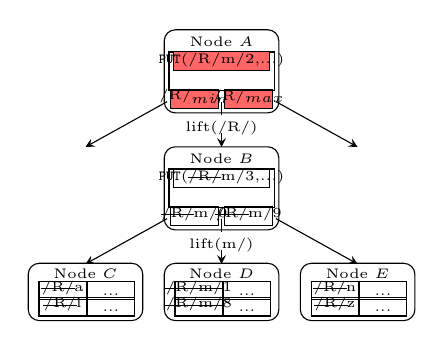
\begin{tikzpicture}[xscale=0.95, yscale=0.95]
            \node[anchor=south, rectangle, rounded corners, minimum height=.06\textwidth, minimum width=.12\textwidth, draw=black] at (0, 0) {};
            \node[anchor=south, font=\tiny] at (0, .036\textwidth) {Node $D$};
            \node[anchor=south, rectangle, minimum height=.015\textwidth, minimum width=.05\textwidth, draw=black] at (-.025\textwidth, .005\textwidth) {};
            \node[anchor=south, font=\tiny] at (-.025\textwidth, 0) {\st{/R/m/}8};
            \node[anchor=south, rectangle, minimum height=.015\textwidth, minimum width=.05\textwidth, draw=black] at (.028\textwidth, .005\textwidth) {};
            \node[anchor=south, font=\tiny] at (.028\textwidth, 0) {...};
            \node[anchor=south, rectangle, minimum height=.015\textwidth, minimum width=.05\textwidth, draw=black] at (-.025\textwidth, .023\textwidth) {};
            \node[anchor=south, font=\tiny] at (-.025\textwidth, .018\textwidth) {\st{/R/m/}1};
            \node[anchor=south, rectangle, minimum height=.015\textwidth, minimum width=.05\textwidth, draw=black] at (.028\textwidth, .023\textwidth) {};
            \node[anchor=south, font=\tiny] at (.028\textwidth, .018\textwidth) {...};

            \node[anchor=south, rectangle, rounded corners, minimum height=.06\textwidth, minimum width=.12\textwidth, draw=black] at (.15\textwidth, 0) {};
            \node[anchor=south, font=\tiny] at (.15\textwidth, .036\textwidth) {Node $E$};
            \node[anchor=south, rectangle, minimum height=.015\textwidth, minimum width=.05\textwidth, draw=black] at (.125\textwidth, .005\textwidth) {};
            \node[anchor=south, font=\tiny] at (.125\textwidth, 0) {\st{/R/}z};
            \node[anchor=south, rectangle, minimum height=.015\textwidth, minimum width=.05\textwidth, draw=black] at (.178\textwidth, .005\textwidth) {};
            \node[anchor=south, font=\tiny] at (.178\textwidth, 0) {...};
            \node[anchor=south, rectangle, minimum height=.015\textwidth, minimum width=.05\textwidth, draw=black] at (.125\textwidth, .023\textwidth) {};
            \node[anchor=south, font=\tiny] at (.125\textwidth, .018\textwidth) {\st{/R/}n};
            \node[anchor=south, rectangle, minimum height=.015\textwidth, minimum width=.05\textwidth, draw=black] at (.178\textwidth, .023\textwidth) {};
            \node[anchor=south, font=\tiny] at (.178\textwidth, .018\textwidth) {...};

            \node[anchor=south, rectangle, rounded corners, minimum height=.06\textwidth, minimum width=.12\textwidth, draw=black] at (-.15\textwidth, 0) {};
            \node[anchor=south, font=\tiny] at (-.15\textwidth, .036\textwidth) {Node $C$};
            \node[anchor=south, rectangle, minimum height=.015\textwidth, minimum width=.05\textwidth, draw=black] at (-.175\textwidth, .005\textwidth) {};
            \node[anchor=south, font=\tiny] at (-.175\textwidth, 0) {\st{/R/}l};
            \node[anchor=south, rectangle, minimum height=.015\textwidth, minimum width=.05\textwidth, draw=black] at (-.122\textwidth, .005\textwidth) {};
            \node[anchor=south, font=\tiny] at (-.122\textwidth, 0) {...};
            \node[anchor=south, rectangle, minimum height=.015\textwidth, minimum width=.05\textwidth, draw=black] at (-.175\textwidth, .023\textwidth) {};
            \node[anchor=south, font=\tiny] at (-.175\textwidth, .018\textwidth) {\st{/R/}a};
            \node[anchor=south, rectangle, minimum height=.015\textwidth, minimum width=.05\textwidth, draw=black] at (-.122\textwidth, .023\textwidth) {};
            \node[anchor=south, font=\tiny] at (-.122\textwidth, .018\textwidth) {...};

            \node[anchor=south, rectangle, rounded corners, minimum height=.087\textwidth, minimum width=.12\textwidth, draw=black] at (0, .1\textwidth) {};
            \node[anchor=south, font=\tiny] at (0, .163\textwidth) {Node $B$};
            \node[anchor=south, rectangle, minimum height=.015\textwidth, minimum width=.05\textwidth, draw=black] at (-.03\textwidth, .105\textwidth) {};
            \node[anchor=south, font=\tiny] at (-.03\textwidth, .1\textwidth) {\st{/R/}m/0};
            \node[anchor=south, rectangle, minimum height=.015\textwidth, minimum width=.05\textwidth, draw=black] at (.03\textwidth, .105\textwidth) {};
            \node[anchor=south, font=\tiny] at (.03\textwidth, .1\textwidth) {\st{/R/}m/9};
            \node[anchor=south, rectangle, minimum height=.04\textwidth, minimum width=.11\textwidth, draw=black] at (0, .125\textwidth) {};
            \node[anchor=south, rectangle, minimum height=.015\textwidth, minimum width=.1\textwidth, draw=black] at (0, .147\textwidth) {};
            \node[anchor=south, font=\tiny] at  (0, .141\textwidth) {\putm(\st{/R/}m/3,...)};

            \node[anchor=south, rectangle, rounded corners, minimum height=.087\textwidth, minimum width=.12\textwidth, draw=black] at (0, .229\textwidth) {};
            \node[anchor=south, font=\tiny] at (0, .292\textwidth) {Node $A$};
            \node[anchor=south, rectangle, minimum height=.015\textwidth, minimum width=.05\textwidth, draw=black, fill={red!60}] at (-.03\textwidth, .234\textwidth) {};
            \node[anchor=south, font=\tiny] at (-.03\textwidth, .229\textwidth) {/R/$_{min}$};
            \node[anchor=south, rectangle, minimum height=.015\textwidth, minimum width=.05\textwidth, draw=black, fill={red!60}] at (.03\textwidth, .234\textwidth) {};
            \node[anchor=south, font=\tiny] at (.03\textwidth, .229\textwidth) {/R/$_{max}$};
            \node[anchor=south, rectangle, minimum height=.04\textwidth, minimum width=.11\textwidth, draw=black] at (0, .254\textwidth) {};
            \node[anchor=south, rectangle, minimum height=.015\textwidth, minimum width=.1\textwidth, draw=black, fill={red!60}] at (0, .276\textwidth) {};
            \node[anchor=south, font=\tiny] at  (0, .27\textwidth) {\putm(/R/m/2,...)};

            \draw[->, >=stealth] (0, .113\textwidth) -- (0, .063\textwidth);
            \draw[->, >=stealth] (.06\textwidth, .113\textwidth) -- (.15\textwidth, .063\textwidth);
            \draw[->, >=stealth] (-.06\textwidth, .113\textwidth) -- (-.15\textwidth, .063\textwidth);
            \draw[->, >=stealth] (0, .242\textwidth) -- (0, .192\textwidth);
            \draw[->, >=stealth] (.06\textwidth, .242\textwidth) -- (.15\textwidth, .192\textwidth);
            \draw[->, >=stealth] (-.06\textwidth, .242\textwidth) -- (-.15\textwidth, .192\textwidth);

            \node[anchor=north,rectangle, minimum height=.015\textwidth, minimum width=.05\textwidth, fill={white}] at (0, .228\textwidth) {};
            \node[anchor=north, font=\tiny] at (0, .231\textwidth) {lift(/R/)};
            \node[anchor=north,rectangle, minimum height=.015\textwidth, minimum width=.05\textwidth, fill={white}] at (0, .099\textwidth) {};
            \node[anchor=north, font=\tiny] at (0, .102\textwidth) {lift(m/)};
        \end{tikzpicture}
        \caption{\label{subfig:lift-1} The lifted \bet that stores the same keys
            in each node. Lifted prefixes are marked as strike-through in keys.}
    \end{subfigure}
    \begin{subfigure}{\textwidth}
        \centering
        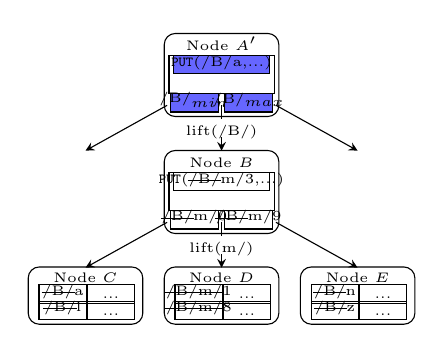
\begin{tikzpicture}[xscale=0.95, yscale=0.95]
            \node[anchor=south, rectangle, rounded corners, minimum height=.06\textwidth, minimum width=.12\textwidth, draw=black] at (0, 0) {};
            \node[anchor=south, font=\tiny] at (0, .036\textwidth) {Node $D$};
            \node[anchor=south, rectangle, minimum height=.015\textwidth, minimum width=.05\textwidth, draw=black] at (-.025\textwidth, .005\textwidth) {};
            \node[anchor=south, font=\tiny] at (-.025\textwidth, 0) {\st{/B/m/}8};
            \node[anchor=south, rectangle, minimum height=.015\textwidth, minimum width=.05\textwidth, draw=black] at (.028\textwidth, .005\textwidth) {};
            \node[anchor=south, font=\tiny] at (.028\textwidth, 0) {...};
            \node[anchor=south, rectangle, minimum height=.015\textwidth, minimum width=.05\textwidth, draw=black] at (-.025\textwidth, .023\textwidth) {};
            \node[anchor=south, font=\tiny] at (-.025\textwidth, .018\textwidth) {\st{/B/m/}1};
            \node[anchor=south, rectangle, minimum height=.015\textwidth, minimum width=.05\textwidth, draw=black] at (.028\textwidth, .023\textwidth) {};
            \node[anchor=south, font=\tiny] at (.028\textwidth, .018\textwidth) {...};

            \node[anchor=south, rectangle, rounded corners, minimum height=.06\textwidth, minimum width=.12\textwidth, draw=black] at (.15\textwidth, 0) {};
            \node[anchor=south, font=\tiny] at (.15\textwidth, .036\textwidth) {Node $E$};
            \node[anchor=south, rectangle, minimum height=.015\textwidth, minimum width=.05\textwidth, draw=black] at (.125\textwidth, .005\textwidth) {};
            \node[anchor=south, font=\tiny] at (.125\textwidth, 0) {\st{/B/}z};
            \node[anchor=south, rectangle, minimum height=.015\textwidth, minimum width=.05\textwidth, draw=black] at (.178\textwidth, .005\textwidth) {};
            \node[anchor=south, font=\tiny] at (.178\textwidth, 0) {...};
            \node[anchor=south, rectangle, minimum height=.015\textwidth, minimum width=.05\textwidth, draw=black] at (.125\textwidth, .023\textwidth) {};
            \node[anchor=south, font=\tiny] at (.125\textwidth, .018\textwidth) {\st{/B/}n};
            \node[anchor=south, rectangle, minimum height=.015\textwidth, minimum width=.05\textwidth, draw=black] at (.178\textwidth, .023\textwidth) {};
            \node[anchor=south, font=\tiny] at (.178\textwidth, .018\textwidth) {...};

            \node[anchor=south, rectangle, rounded corners, minimum height=.06\textwidth, minimum width=.12\textwidth, draw=black] at (-.15\textwidth, 0) {};
            \node[anchor=south, font=\tiny] at (-.15\textwidth, .036\textwidth) {Node $C$};
            \node[anchor=south, rectangle, minimum height=.015\textwidth, minimum width=.05\textwidth, draw=black] at (-.175\textwidth, .005\textwidth) {};
            \node[anchor=south, font=\tiny] at (-.175\textwidth, 0) {\st{/B/}l};
            \node[anchor=south, rectangle, minimum height=.015\textwidth, minimum width=.05\textwidth, draw=black] at (-.122\textwidth, .005\textwidth) {};
            \node[anchor=south, font=\tiny] at (-.122\textwidth, 0) {...};
            \node[anchor=south, rectangle, minimum height=.015\textwidth, minimum width=.05\textwidth, draw=black] at (-.175\textwidth, .023\textwidth) {};
            \node[anchor=south, font=\tiny] at (-.175\textwidth, .018\textwidth) {\st{/B/}a};
            \node[anchor=south, rectangle, minimum height=.015\textwidth, minimum width=.05\textwidth, draw=black] at (-.122\textwidth, .023\textwidth) {};
            \node[anchor=south, font=\tiny] at (-.122\textwidth, .018\textwidth) {...};

            \node[anchor=south, rectangle, rounded corners, minimum height=.087\textwidth, minimum width=.12\textwidth, draw=black] at (0, .1\textwidth) {};
            \node[anchor=south, font=\tiny] at (0, .163\textwidth) {Node $B$};
            \node[anchor=south, rectangle, minimum height=.015\textwidth, minimum width=.05\textwidth, draw=black] at (-.03\textwidth, .105\textwidth) {};
            \node[anchor=south, font=\tiny] at (-.03\textwidth, .1\textwidth) {\st{/B/}m/0};
            \node[anchor=south, rectangle, minimum height=.015\textwidth, minimum width=.05\textwidth, draw=black] at (.03\textwidth, .105\textwidth) {};
            \node[anchor=south, font=\tiny] at (.03\textwidth, .1\textwidth) {\st{/B/}m/9};
            \node[anchor=south, rectangle, minimum height=.04\textwidth, minimum width=.11\textwidth, draw=black] at (0, .125\textwidth) {};
            \node[anchor=south, rectangle, minimum height=.015\textwidth, minimum width=.1\textwidth, draw=black] at (0, .147\textwidth) {};
            \node[anchor=south, font=\tiny] at  (0, .141\textwidth) {\putm(\st{/B/}m/3,...)};

            \node[anchor=south, rectangle, rounded corners, minimum height=.087\textwidth, minimum width=.12\textwidth, draw=black] at (0, .229\textwidth) {};
            \node[anchor=south, font=\tiny] at (0, .292\textwidth) {Node $A'$};
            \node[anchor=south, rectangle, minimum height=.015\textwidth, minimum width=.05\textwidth, draw=black, fill={blue!60}] at (-.03\textwidth, .234\textwidth) {};
            \node[anchor=south, font=\tiny] at (-.03\textwidth, .229\textwidth) {/B/$_{min}$};
            \node[anchor=south, rectangle, minimum height=.015\textwidth, minimum width=.05\textwidth, draw=black, fill={blue!60}] at (.03\textwidth, .234\textwidth) {};
            \node[anchor=south, font=\tiny] at (.03\textwidth, .229\textwidth) {/B/$_{max}$};
            \node[anchor=south, rectangle, minimum height=.04\textwidth, minimum width=.11\textwidth, draw=black] at (0, .254\textwidth) {};
            \node[anchor=south, rectangle, minimum height=.015\textwidth, minimum width=.1\textwidth, draw=black, fill={blue!60}] at (0, .276\textwidth) {};
            \node[anchor=south, font=\tiny] at  (0, .27\textwidth) {\putm(/B/a,...)};

            \draw[->, >=stealth] (0, .113\textwidth) -- (0, .063\textwidth);
            \draw[->, >=stealth] (.06\textwidth, .113\textwidth) -- (.15\textwidth, .063\textwidth);
            \draw[->, >=stealth] (-.06\textwidth, .113\textwidth) -- (-.15\textwidth, .063\textwidth);
            \draw[->, >=stealth] (0, .242\textwidth) -- (0, .192\textwidth);
            \draw[->, >=stealth] (.06\textwidth, .242\textwidth) -- (.15\textwidth, .192\textwidth);
            \draw[->, >=stealth] (-.06\textwidth, .242\textwidth) -- (-.15\textwidth, .192\textwidth);

            \node[anchor=north,rectangle, minimum height=.015\textwidth, minimum width=.05\textwidth, fill={white}] at (0, .228\textwidth) {};
            \node[anchor=north, font=\tiny] at (0, .231\textwidth) {lift(/B/)};
            \node[anchor=north,rectangle, minimum height=.015\textwidth, minimum width=.05\textwidth, fill={white}] at (0, .099\textwidth) {};
            \node[anchor=north, font=\tiny] at (0, .102\textwidth) {lift(m/)};
        \end{tikzpicture}
        \caption{\label{subfig:lift-2} When the subtree rooted at Node $B$ is
            bounded by two different pivots, all keys in the subtree change
            their prefixes.}
    \end{subfigure}
    \caption[An key lifting example]{\label{fig:lift}
        Key lifting lifts prefixes from the subtree. Keys in the same subtree
        are viewed with different prefixes when the pivots in its parent
        change.}
\end{figure}

After tree surgery, one can move the isolated subtree to another location in
the \bet.
However, the keys in the subtree will not be coherent with the new location in
the tree.
Thus, as a part of the range-rename operation, the prefixes of keys in this
subtree need to be updated.
A naive approach will traverse the subtree and update all keys.
However, this process costs a lot of I/Os, rewriting every node in the source
subtree.
The particularly concerning case is when the subtree is very large.

Key lifting eliminates the need to update prefixes of keys in the subtree by
transforming \bets into lifted \bets.
The idea of key lifting comes from the observation that with lexicographic key
order, all keys bounded in the key range of two pivots must have the same prefix
that is the \textbf{LCP} (Longest Common Prefix) of the pivots.
Therefore, this LCP is redundant information in the subtree of the two pivots
and can be removed from the subtree.
In particular, the subtree generated by tree surgery is bounded by two pivots,
$p_{min}$ and $p_{max}$ and with lexicographic key order, all keys in the
subtree must have prefix $p$.

In lifted \bets, a parent-to-child pointer lifts the LCP of the two pivots from
the subtree rooted at the child.
Child nodes only store differing key suffixes.
This approach encodes the complete key in the path taken to reach a given node
and one can then modify the prefix for a lifted subtree by only modifying the
parent node, eliminating the need to change key and pivot prefixes in all nodes
of a subtree.

Figure~\ref{fig:lift} shows an example of key lifting.
Figure~\ref{subfig:lift-0} and Figure~\ref{subfig:lift-1} show the same \bet
with and without key lifting, respectively.
In Figure~\ref{subfig:lift-1}, the subtree rooted at Node $B$ is
bounded by two pivots, ``/R/$_{min}$'' and ``/R/$_{max}$'', in Node $A$.
Therefore, all keys in the subtree must have prefix ``/R/'' and key lifting
removes this prefix from the subtree
(we show the lifted prefix on the parent-to-child pointer and mark the lifted
prefix as strike-through in the subtree).
Because keys in Node $B$ don't have prefix ``/R/'' physically in the node,
we show transparent keys (``/R/'' keys are red in previous examples) in the node.
Likewise, Node $D$ is bounded by ``m/a'' and ``m/z'' in Node $B$
(note ``/R/'' is already lifted from the sutbree rooted at Node $B$),
so key lifting removes prefix ``m/'' from Node $D$.
In Figure~\ref{subfig:lift-2}, the same subtree, which contains exactly the
same key/value pairs, is moved to a different location, bounded by two new
pivots, ``/B/$_{min}$'' and ``/B/$_{max}$'', in Node $A'$.
Because the prefix lifted through the parent-to-child pointer in Node $A'$
becomes ``/B/'', all keys in the subtree have prefix ``/B/'' instead.
For examples in the rest of the dissertation, we will not show lifted prefixes
in keys.

A query on a lifted \bet needs to track lifted prefixes during the
root-to-leaf traversal and reconstruct the full key by concatenating these
prefixes and the suffix in the leaf.
For example, consider a query for key ``/R/m/1'' in Figure~\ref{subfig:lift-1}.
When following the parent-to-child pointer from Node $A$ to Node $B$,
the query notices the lifted prefix ``/R/''.
Therefore, the query searches for key ``m/1'' in Node $B$ and follows the
parent-to-child pointer to Node $D$.
Again, the query removes the lifted prefix, ``m/'', from the search key.
After fetching the key/value pair of key ``1'' in Node $D$, the query prepends
prefixes lifted long the root-to-leaf path and recovers the full key ``/R/m/1''.
Note the recovering process is not necessary for point queries because they know
their keys beforehand, but range queries must reconstruct the resulting keys.

Also, a lifted \bet must remove the lifted prefix from a message before flushing
the message from parent to child.
For example, in Figure~\ref{subfig:lift-1}, when flushing the message
\putm(``/R/m/2'',...) from Node $A$ to Node $B$, the lifted \bet remove the
prefix ``/R/'' from the message and injects a message \putm(``m/2'',...) into
the buffer of Node $B$.

A node split in a lifted \bet adds a pivot to the parent, which may change
the lifted prefix associated with the parent-to-child pointer, so it may need to
update keys in the resulting children.
Similarly, a node merge needs to re-lift keys in the resulting node.

However, the extra work described above for \bet operations can be resolved in
memory.
Therefore, key lifting doesn't incur additional I/Os for other \bet operations.

Compared to zoning, in which the file system removes certain prefixes from keys,
key lifting is completely transparent to \betrfs.
\betrfs still stores key/value pairs with full-path keys,
just with a slightly different data structure.

\subsection{The range-rename operation on lifted \bets}
\label{sec:rr:op:rr}

\begin{figure}
    \begin{subfigure}{\textwidth}
        \centering
        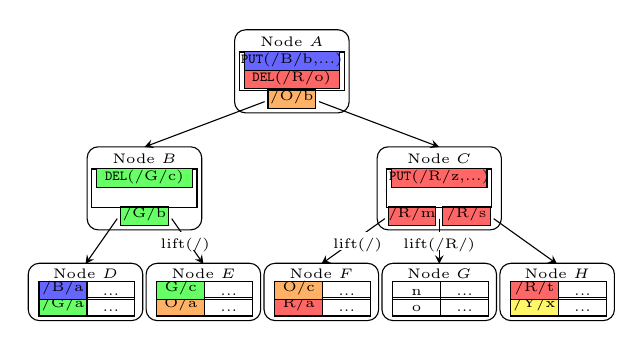
\begin{tikzpicture}[xscale=0.95, yscale=0.95]
            \node[anchor=south, rectangle, rounded corners, minimum height=.06\textwidth, minimum width=.12\textwidth, draw=black] at (0, 0) {};
            \node[anchor=south, font=\tiny] at (0, .036\textwidth) {Node $F$};
            \node[anchor=south, rectangle, minimum height=.015\textwidth, minimum width=.05\textwidth, draw=black, fill={red!60}] at (-.025\textwidth, .005\textwidth) {};
            \node[anchor=south, font=\tiny] at (-.025\textwidth, 0) {R/a};
            \node[anchor=south, rectangle, minimum height=.015\textwidth, minimum width=.05\textwidth, draw=black] at (.028\textwidth, .005\textwidth) {};
            \node[anchor=south, font=\tiny] at (.028\textwidth, 0) {...};
            \node[anchor=south, rectangle, minimum height=.015\textwidth, minimum width=.05\textwidth, draw=black, fill={orange!60}] at (-.025\textwidth, .023\textwidth) {};
            \node[anchor=south, font=\tiny] at (-.025\textwidth, .018\textwidth) {O/c};
            \node[anchor=south, rectangle, minimum height=.015\textwidth, minimum width=.05\textwidth, draw=black] at (.028\textwidth, .023\textwidth) {};
            \node[anchor=south, font=\tiny] at (.028\textwidth, .018\textwidth) {...};

            \node[anchor=south, rectangle, rounded corners, minimum height=.06\textwidth, minimum width=.12\textwidth, draw=black] at (.13\textwidth, 0) {};
            \node[anchor=south, font=\tiny] at (.13\textwidth, .036\textwidth) {Node $G$};
            \node[anchor=south, rectangle, minimum height=.015\textwidth, minimum width=.05\textwidth, draw=black] at (.105\textwidth, .005\textwidth) {};
            \node[anchor=south, font=\tiny] at (.105\textwidth, 0) {o};
            \node[anchor=south, rectangle, minimum height=.015\textwidth, minimum width=.05\textwidth, draw=black] at (.158\textwidth, .005\textwidth) {};
            \node[anchor=south, font=\tiny] at (.158\textwidth, 0) {...};
            \node[anchor=south, rectangle, minimum height=.015\textwidth, minimum width=.05\textwidth, draw=black] at (.105\textwidth, .023\textwidth) {};
            \node[anchor=south, font=\tiny] at (.105\textwidth, .018\textwidth) {n};
            \node[anchor=south, rectangle, minimum height=.015\textwidth, minimum width=.05\textwidth, draw=black] at (.158\textwidth, .023\textwidth) {};
            \node[anchor=south, font=\tiny] at (.158\textwidth, .018\textwidth) {...};

            \node[anchor=south, rectangle, rounded corners, minimum height=.06\textwidth, minimum width=.12\textwidth, draw=black] at (.26\textwidth, 0) {};
            \node[anchor=south, font=\tiny] at (.26\textwidth, .036\textwidth) {Node $H$};
            \node[anchor=south, rectangle, minimum height=.015\textwidth, minimum width=.05\textwidth, draw=black, fill={yellow!60}] at (.235\textwidth, .005\textwidth) {};
            \node[anchor=south, font=\tiny] at (.235\textwidth, 0) {/Y/x};
            \node[anchor=south, rectangle, minimum height=.015\textwidth, minimum width=.05\textwidth, draw=black] at (.288\textwidth, .005\textwidth) {};
            \node[anchor=south, font=\tiny] at (.288\textwidth, 0) {...};
            \node[anchor=south, rectangle, minimum height=.015\textwidth, minimum width=.05\textwidth, draw=black, fill={red!60}] at (.235\textwidth, .023\textwidth) {};
            \node[anchor=south, font=\tiny] at (.235\textwidth, .018\textwidth) {/R/t};
            \node[anchor=south, rectangle, minimum height=.015\textwidth, minimum width=.05\textwidth, draw=black] at (.288\textwidth, .023\textwidth) {};
            \node[anchor=south, font=\tiny] at (.288\textwidth, .018\textwidth) {...};

            \node[anchor=south, rectangle, rounded corners, minimum height=.06\textwidth, minimum width=.12\textwidth, draw=black] at (-.13\textwidth, 0) {};
            \node[anchor=south, font=\tiny] at (-.13\textwidth, .036\textwidth) {Node $E$};
            \node[anchor=south, rectangle, minimum height=.015\textwidth, minimum width=.05\textwidth, draw=black, fill={orange!60}] at (-.155\textwidth, .005\textwidth) {};
            \node[anchor=south, font=\tiny] at (-.155\textwidth, 0) {O/a};
            \node[anchor=south, rectangle, minimum height=.015\textwidth, minimum width=.05\textwidth, draw=black] at (-.102\textwidth, .005\textwidth) {};
            \node[anchor=south, font=\tiny] at (-.102\textwidth, 0) {...};
            \node[anchor=south, rectangle, minimum height=.015\textwidth, minimum width=.05\textwidth, draw=black, fill={green!60}] at (-.155\textwidth, .023\textwidth) {};
            \node[anchor=south, font=\tiny] at (-.155\textwidth, .018\textwidth) {G/c};
            \node[anchor=south, rectangle, minimum height=.015\textwidth, minimum width=.05\textwidth, draw=black] at (-.102\textwidth, .023\textwidth) {};
            \node[anchor=south, font=\tiny] at (-.102\textwidth, .018\textwidth) {...};

            \node[anchor=south, rectangle, rounded corners, minimum height=.06\textwidth, minimum width=.12\textwidth, draw=black] at (-.26\textwidth, 0) {};
            \node[anchor=south, font=\tiny] at (-.26\textwidth, .036\textwidth) {Node $D$};
            \node[anchor=south, rectangle, minimum height=.015\textwidth, minimum width=.05\textwidth, draw=black, fill={green!60}] at (-.285\textwidth, .005\textwidth) {};
            \node[anchor=south, font=\tiny] at (-.285\textwidth, 0) {/G/a};
            \node[anchor=south, rectangle, minimum height=.015\textwidth, minimum width=.05\textwidth, draw=black] at (-.232\textwidth, .005\textwidth) {};
            \node[anchor=south, font=\tiny] at (-.232\textwidth, 0) {...};
            \node[anchor=south, rectangle, minimum height=.015\textwidth, minimum width=.05\textwidth, draw=black, fill={blue!60}] at (-.285\textwidth, .023\textwidth) {};
            \node[anchor=south, font=\tiny] at (-.285\textwidth, .018\textwidth) {/B/a};
            \node[anchor=south, rectangle, minimum height=.015\textwidth, minimum width=.05\textwidth, draw=black] at (-.232\textwidth, .023\textwidth) {};
            \node[anchor=south, font=\tiny] at (-.232\textwidth, .018\textwidth) {...};

            \node[anchor=south, rectangle, rounded corners, minimum height=.087\textwidth, minimum width=.12\textwidth, draw=black] at (-.195\textwidth, .1\textwidth) {};
            \node[anchor=south, font=\tiny] at (-.195\textwidth, .163\textwidth) {Node $B$};
            \node[anchor=south, rectangle, minimum height=.015\textwidth, minimum width=.05\textwidth, draw=black, fill={green!60}] at (-.195\textwidth, .105\textwidth) {};
            \node[anchor=south, font=\tiny] at (-.195\textwidth, .1\textwidth) {/G/b};
            \node[anchor=south, rectangle, minimum height=.04\textwidth, minimum width=.11\textwidth, draw=black] at (-.195\textwidth, .125\textwidth) {};
            \node[anchor=south, rectangle, minimum height=.015\textwidth, minimum width=.1\textwidth, draw=black, fill={green!60}] at (-.195\textwidth, .147\textwidth) {};
            \node[anchor=south, font=\tiny] at  (-.195\textwidth, .141\textwidth) {\delm(/G/c)};

            \node[anchor=south, rectangle, rounded corners, minimum height=.087\textwidth, minimum width=.13\textwidth, draw=black] at (.13\textwidth, .1\textwidth) {};
            \node[anchor=south, font=\tiny] at (.13\textwidth, .163\textwidth) {Node $C$};
            \node[anchor=south, rectangle, minimum height=.015\textwidth, minimum width=.05\textwidth, draw=black, fill={red!60}] at (.1\textwidth, .105\textwidth) {};
            \node[anchor=south, font=\tiny] at (.1\textwidth, .1\textwidth) {/R/m};
            \node[anchor=south, rectangle, minimum height=.015\textwidth, minimum width=.05\textwidth, draw=black, fill={red!60}] at (.16\textwidth, .105\textwidth) {};
            \node[anchor=south, font=\tiny] at (.16\textwidth, .1\textwidth) {/R/s};
            \node[anchor=south, rectangle, minimum height=.04\textwidth, minimum width=.11\textwidth, draw=black] at (.13\textwidth, .125\textwidth) {};
            \node[anchor=south, rectangle, minimum height=.015\textwidth, minimum width=.1\textwidth, draw=black, fill={red!60}] at (.13\textwidth, .147\textwidth) {};
            \node[anchor=south, font=\tiny] at  (.13\textwidth, .141\textwidth) {\putm(/R/z,...)};

            \node[anchor=south, rectangle, rounded corners, minimum height=.087\textwidth, minimum width=.12\textwidth, draw=black] at (-.0325\textwidth, .229\textwidth) {};
            \node[anchor=south, font=\tiny] at (-.0325\textwidth, .292\textwidth) {Node $A$};
            \node[anchor=south, rectangle, minimum height=.015\textwidth, minimum width=.05\textwidth, draw=black, fill={orange!60}] at (-.0325\textwidth, .234\textwidth) {};
            \node[anchor=south, font=\tiny] at (-.0325\textwidth, .229\textwidth) {/O/b};
            \node[anchor=south, rectangle, minimum height=.04\textwidth, minimum width=.11\textwidth, draw=black] at (-.0325\textwidth, .254\textwidth) {};
            \node[anchor=south, rectangle, minimum height=.015\textwidth, minimum width=.1\textwidth, draw=black, fill={red!60}] at (-.0325\textwidth, .256\textwidth) {};
            \node[anchor=south, font=\tiny] at  (-.0325\textwidth, .25\textwidth) {\delm(/R/o)};
            \node[anchor=south, rectangle, minimum height=.015\textwidth, minimum width=.1\textwidth, draw=black, fill={blue!60}] at (-.0325\textwidth, .276\textwidth) {};
            \node[anchor=south, font=\tiny] at  (-.0325\textwidth, .27\textwidth) {\putm(/B/b,...)};

            \draw[->, >=stealth] (-.225\textwidth, .113\textwidth) -- (-.26\textwidth, .063\textwidth);
            \draw[->, >=stealth] (-.165\textwidth, .113\textwidth) -- (-.13\textwidth, .063\textwidth);
            \draw[->, >=stealth] (.13\textwidth, .113\textwidth) -- (.13\textwidth, .063\textwidth);
            \draw[->, >=stealth] (.19\textwidth, .113\textwidth) -- (.26\textwidth, .063\textwidth);
            \draw[->, >=stealth] (.07\textwidth, .113\textwidth) -- (0, .063\textwidth);
            \draw[->, >=stealth] (-.0625\textwidth, .242\textwidth) -- (-.195\textwidth, .192\textwidth);
            \draw[->, >=stealth] (-.0025\textwidth, .242\textwidth) -- (.13\textwidth, .192\textwidth);

            \node[anchor=north,rectangle, minimum height=.015\textwidth, minimum width=.05\textwidth, fill={white}] at (.13\textwidth, .099\textwidth) {};
            \node[anchor=north, font=\tiny] at (.13\textwidth, .102\textwidth) {lift(/R/)};
            \node[anchor=north,rectangle, minimum height=.015\textwidth, minimum width=.05\textwidth, fill={white}] at (.04\textwidth, .099\textwidth) {};
            \node[anchor=north, font=\tiny] at (.04\textwidth, .102\textwidth) {lift(/)};
            \node[anchor=north,rectangle, minimum height=.015\textwidth, minimum width=.05\textwidth, fill={white}] at (-.15\textwidth, .099\textwidth) {};
            \node[anchor=north, font=\tiny] at (-.15\textwidth, .102\textwidth) {lift(/)};
        \end{tikzpicture}
        \caption{\label{subfig:rr-1} The \bet before the range-rename operation.}
    \end{subfigure}
    \begin{subfigure}{\textwidth}
        \centering
        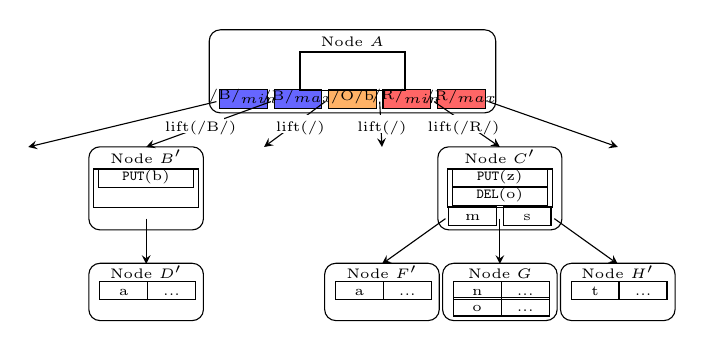
\begin{tikzpicture}[xscale=0.95, yscale=0.95]
            \node[anchor=south, rectangle, rounded corners, minimum height=.06\textwidth, minimum width=.12\textwidth, draw=black] at (0, 0) {};
            \node[anchor=south, font=\tiny] at (0, .036\textwidth) {Node $F'$};
            \node[anchor=south, rectangle, minimum height=.015\textwidth, minimum width=.05\textwidth, draw=black] at (-.025\textwidth, .023\textwidth) {};
            \node[anchor=south, font=\tiny] at (-.025\textwidth, .018\textwidth) {a};
            \node[anchor=south, rectangle, minimum height=.015\textwidth, minimum width=.05\textwidth, draw=black] at (.028\textwidth, .023\textwidth) {};
            \node[anchor=south, font=\tiny] at (.028\textwidth, .018\textwidth) {...};

            \node[anchor=south, rectangle, rounded corners, minimum height=.06\textwidth, minimum width=.12\textwidth, draw=black] at (.13\textwidth, 0) {};
            \node[anchor=south, font=\tiny] at (.13\textwidth, .036\textwidth) {Node $G$};
            \node[anchor=south, rectangle, minimum height=.015\textwidth, minimum width=.05\textwidth, draw=black] at (.105\textwidth, .005\textwidth) {};
            \node[anchor=south, font=\tiny] at (.105\textwidth, 0) {o};
            \node[anchor=south, rectangle, minimum height=.015\textwidth, minimum width=.05\textwidth, draw=black] at (.158\textwidth, .005\textwidth) {};
            \node[anchor=south, font=\tiny] at (.158\textwidth, 0) {...};
            \node[anchor=south, rectangle, minimum height=.015\textwidth, minimum width=.05\textwidth, draw=black] at (.105\textwidth, .023\textwidth) {};
            \node[anchor=south, font=\tiny] at (.105\textwidth, .018\textwidth) {n};
            \node[anchor=south, rectangle, minimum height=.015\textwidth, minimum width=.05\textwidth, draw=black] at (.158\textwidth, .023\textwidth) {};
            \node[anchor=south, font=\tiny] at (.158\textwidth, .018\textwidth) {...};

            \node[anchor=south, rectangle, rounded corners, minimum height=.06\textwidth, minimum width=.12\textwidth, draw=black] at (.26\textwidth, 0) {};
            \node[anchor=south, font=\tiny] at (.26\textwidth, .036\textwidth) {Node $H'$};
            \node[anchor=south, rectangle, minimum height=.015\textwidth, minimum width=.05\textwidth, draw=black] at (.235\textwidth, .023\textwidth) {};
            \node[anchor=south, font=\tiny] at (.235\textwidth, .018\textwidth) {t};
            \node[anchor=south, rectangle, minimum height=.015\textwidth, minimum width=.05\textwidth, draw=black] at (.288\textwidth, .023\textwidth) {};
            \node[anchor=south, font=\tiny] at (.288\textwidth, .018\textwidth) {...};

            \node[anchor=south, rectangle, rounded corners, minimum height=.06\textwidth, minimum width=.12\textwidth, draw=black] at (-.26\textwidth, 0) {};
            \node[anchor=south, font=\tiny] at (-.26\textwidth, .036\textwidth) {Node $D'$};
            \node[anchor=south, rectangle, minimum height=.015\textwidth, minimum width=.05\textwidth, draw=black] at (-.285\textwidth, .023\textwidth) {};
            \node[anchor=south, font=\tiny] at (-.285\textwidth, .018\textwidth) {a};
            \node[anchor=south, rectangle, minimum height=.015\textwidth, minimum width=.05\textwidth, draw=black] at (-.232\textwidth, .023\textwidth) {};
            \node[anchor=south, font=\tiny] at (-.232\textwidth, .018\textwidth) {...};

            \node[anchor=south, rectangle, rounded corners, minimum height=.087\textwidth, minimum width=.12\textwidth, draw=black] at (-.26\textwidth, .1\textwidth) {};
            \node[anchor=south, font=\tiny] at (-.26\textwidth, .163\textwidth) {Node $B'$};
            \node[anchor=south, rectangle, minimum height=.04\textwidth, minimum width=.11\textwidth, draw=black] at (-.26\textwidth, .125\textwidth) {};
            \node[anchor=south, rectangle, minimum height=.015\textwidth, minimum width=.1\textwidth, draw=black] at (-.26\textwidth, .147\textwidth) {};
            \node[anchor=south, font=\tiny] at  (-.26\textwidth, .141\textwidth) {\putm(b)};

            \node[anchor=south, rectangle, rounded corners, minimum height=.087\textwidth, minimum width=.13\textwidth, draw=black] at (.13\textwidth, .1\textwidth) {};
            \node[anchor=south, font=\tiny] at (.13\textwidth, .163\textwidth) {Node $C'$};
            \node[anchor=south, rectangle, minimum height=.015\textwidth, minimum width=.05\textwidth, draw=black] at (.1\textwidth, .105\textwidth) {};
            \node[anchor=south, font=\tiny] at (.1\textwidth, .1\textwidth) {m};
            \node[anchor=south, rectangle, minimum height=.015\textwidth, minimum width=.05\textwidth, draw=black] at (.16\textwidth, .105\textwidth) {};
            \node[anchor=south, font=\tiny] at (.16\textwidth, .1\textwidth) {s};
            \node[anchor=south, rectangle, minimum height=.04\textwidth, minimum width=.11\textwidth, draw=black] at (.13\textwidth, .125\textwidth) {};
            \node[anchor=south, rectangle, minimum height=.015\textwidth, minimum width=.1\textwidth, draw=black] at (.13\textwidth, .147\textwidth) {};
            \node[anchor=south, font=\tiny] at  (.13\textwidth, .141\textwidth) {\putm(z)};
            \node[anchor=south, rectangle, minimum height=.015\textwidth, minimum width=.1\textwidth, draw=black] at (.13\textwidth, .127\textwidth) {};
            \node[anchor=south, font=\tiny] at  (.13\textwidth, .121\textwidth) {\delm(o)};

            \node[anchor=south, rectangle, rounded corners, minimum height=.087\textwidth, minimum width=.3\textwidth, draw=black] at (-.0325\textwidth, .229\textwidth) {};
            \node[anchor=south, font=\tiny] at (-.0325\textwidth, .292\textwidth) {Node $A$};
            \node[anchor=south, rectangle, minimum height=.015\textwidth, minimum width=.05\textwidth, draw=black, fill={blue!60}] at (-.1525\textwidth, .234\textwidth) {};
            \node[anchor=south, font=\tiny] at (-.1525\textwidth, .229\textwidth) {/B/$_{min}$};
            \node[anchor=south, rectangle, minimum height=.015\textwidth, minimum width=.05\textwidth, draw=black, fill={blue!60}] at (-.0925\textwidth, .234\textwidth) {};
            \node[anchor=south, font=\tiny] at (-.0925\textwidth, .229\textwidth) {/B/$_{max}$};
            \node[anchor=south, rectangle, minimum height=.015\textwidth, minimum width=.05\textwidth, draw=black, fill={orange!60}] at (-.0325\textwidth, .234\textwidth) {};
            \node[anchor=south, font=\tiny] at (-.0325\textwidth, .229\textwidth) {/O/b};
            \node[anchor=south, rectangle, minimum height=.015\textwidth, minimum width=.05\textwidth, draw=black, fill={red!60}] at (.0275\textwidth, .234\textwidth) {};
            \node[anchor=south, font=\tiny] at (.0275\textwidth, .229\textwidth) {/R/$_{min}$};
            \node[anchor=south, rectangle, minimum height=.015\textwidth, minimum width=.05\textwidth, draw=black, fill={red!60}] at (.0875\textwidth, .234\textwidth) {};
            \node[anchor=south, font=\tiny] at (.0875\textwidth, .229\textwidth) {/R/$_{max}$};
            \node[anchor=south, rectangle, minimum height=.04\textwidth, minimum width=.11\textwidth, draw=black] at (-.0325\textwidth, .254\textwidth) {};

            \draw[->, >=stealth] (-.26\textwidth, .113\textwidth) -- (-.26\textwidth, .063\textwidth);
            \draw[->, >=stealth] (.13\textwidth, .113\textwidth) -- (.13\textwidth, .063\textwidth);
            \draw[->, >=stealth] (.19\textwidth, .113\textwidth) -- (.26\textwidth, .063\textwidth);
            \draw[->, >=stealth] (.07\textwidth, .113\textwidth) -- (0, .063\textwidth);
            \draw[->, >=stealth] (-.1825\textwidth, .242\textwidth) -- (-.39\textwidth, .192\textwidth);
            \draw[->, >=stealth] (-.1225\textwidth, .242\textwidth) -- (-.26\textwidth, .192\textwidth);
            \draw[->, >=stealth] (-.0625\textwidth, .242\textwidth) -- (-.13\textwidth, .192\textwidth);
            \draw[->, >=stealth] (-.0025\textwidth, .242\textwidth) -- (0, .192\textwidth);
            \draw[->, >=stealth] (.0575\textwidth, .242\textwidth) -- (.13\textwidth, .192\textwidth);
            \draw[->, >=stealth] (.1175\textwidth, .242\textwidth) -- (.26\textwidth, .192\textwidth);

            \node[anchor=north,rectangle, minimum height=.015\textwidth, minimum width=.05\textwidth, fill={white}] at (-.20\textwidth, .228\textwidth) {};
            \node[anchor=north, font=\tiny] at (-.20\textwidth, .231\textwidth) {lift(/B/)};
            \node[anchor=north,rectangle, minimum height=.015\textwidth, minimum width=.05\textwidth, fill={white}] at (-.09\textwidth, .228\textwidth) {};
            \node[anchor=north, font=\tiny] at (-.09\textwidth, .231\textwidth) {lift(/)};
            \node[anchor=north,rectangle, minimum height=.015\textwidth, minimum width=.05\textwidth, fill={white}] at (0, .228\textwidth) {};
            \node[anchor=north, font=\tiny] at (0, .231\textwidth) {lift(/)};
            \node[anchor=north,rectangle, minimum height=.015\textwidth, minimum width=.05\textwidth, fill={white}] at (.09\textwidth, .228\textwidth) {};
            \node[anchor=north, font=\tiny] at (.09\textwidth, .231\textwidth) {lift(/R/)};
        \end{tikzpicture}
        \caption{\label{subfig:rr-2} The range-rename operations performs tree surgery
            to slice out the source and destination subtrees.}
    \end{subfigure}
    \begin{subfigure}{\textwidth}
        \centering
        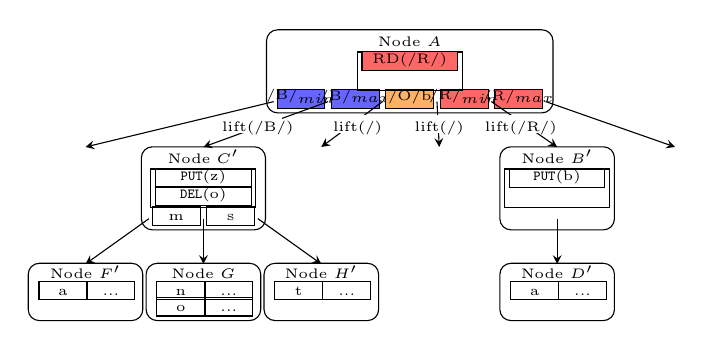
\begin{tikzpicture}[xscale=0.95, yscale=0.95]
            \node[anchor=south, rectangle, rounded corners, minimum height=.06\textwidth, minimum width=.12\textwidth, draw=black] at (-.39\textwidth, 0) {};
            \node[anchor=south, font=\tiny] at (-.39\textwidth, .036\textwidth) {Node $F'$};
            \node[anchor=south, rectangle, minimum height=.015\textwidth, minimum width=.05\textwidth, draw=black] at (-.415\textwidth, .023\textwidth) {};
            \node[anchor=south, font=\tiny] at (-.415\textwidth, .018\textwidth) {a};
            \node[anchor=south, rectangle, minimum height=.015\textwidth, minimum width=.05\textwidth, draw=black] at (-.362\textwidth, .023\textwidth) {};
            \node[anchor=south, font=\tiny] at (-.362\textwidth, .018\textwidth) {...};

            \node[anchor=south, rectangle, rounded corners, minimum height=.06\textwidth, minimum width=.12\textwidth, draw=black] at (-.26\textwidth, 0) {};
            \node[anchor=south, font=\tiny] at (-.26\textwidth, .036\textwidth) {Node $G$};
            \node[anchor=south, rectangle, minimum height=.015\textwidth, minimum width=.05\textwidth, draw=black] at (-.285\textwidth, .005\textwidth) {};
            \node[anchor=south, font=\tiny] at (-.285\textwidth, 0) {o};
            \node[anchor=south, rectangle, minimum height=.015\textwidth, minimum width=.05\textwidth, draw=black] at (-.232\textwidth, .005\textwidth) {};
            \node[anchor=south, font=\tiny] at (-.232\textwidth, 0) {...};
            \node[anchor=south, rectangle, minimum height=.015\textwidth, minimum width=.05\textwidth, draw=black] at (-.285\textwidth, .023\textwidth) {};
            \node[anchor=south, font=\tiny] at (-.285\textwidth, .018\textwidth) {n};
            \node[anchor=south, rectangle, minimum height=.015\textwidth, minimum width=.05\textwidth, draw=black] at (-.232\textwidth, .023\textwidth) {};
            \node[anchor=south, font=\tiny] at (-.232\textwidth, .018\textwidth) {...};

            \node[anchor=south, rectangle, rounded corners, minimum height=.06\textwidth, minimum width=.12\textwidth, draw=black] at (-.13\textwidth, 0) {};
            \node[anchor=south, font=\tiny] at (-.13\textwidth, .036\textwidth) {Node $H'$};
            \node[anchor=south, rectangle, minimum height=.015\textwidth, minimum width=.05\textwidth, draw=black] at (-.155\textwidth, .023\textwidth) {};
            \node[anchor=south, font=\tiny] at (-.155\textwidth, .018\textwidth) {t};
            \node[anchor=south, rectangle, minimum height=.015\textwidth, minimum width=.05\textwidth, draw=black] at (-.102\textwidth, .023\textwidth) {};
            \node[anchor=south, font=\tiny] at (-.102\textwidth, .018\textwidth) {...};

            \node[anchor=south, rectangle, rounded corners, minimum height=.06\textwidth, minimum width=.12\textwidth, draw=black] at (.13\textwidth, 0) {};
            \node[anchor=south, font=\tiny] at (.13\textwidth, .036\textwidth) {Node $D'$};
            \node[anchor=south, rectangle, minimum height=.015\textwidth, minimum width=.05\textwidth, draw=black] at (.105\textwidth, .023\textwidth) {};
            \node[anchor=south, font=\tiny] at (.105\textwidth, .018\textwidth) {a};
            \node[anchor=south, rectangle, minimum height=.015\textwidth, minimum width=.05\textwidth, draw=black] at (.158\textwidth, .023\textwidth) {};
            \node[anchor=south, font=\tiny] at (.158\textwidth, .018\textwidth) {...};

            \node[anchor=south, rectangle, rounded corners, minimum height=.087\textwidth, minimum width=.12\textwidth, draw=black] at (.13\textwidth, .1\textwidth) {};
            \node[anchor=south, font=\tiny] at (.13\textwidth, .163\textwidth) {Node $B'$};
            \node[anchor=south, rectangle, minimum height=.04\textwidth, minimum width=.11\textwidth, draw=black] at (.13\textwidth, .125\textwidth) {};
            \node[anchor=south, rectangle, minimum height=.015\textwidth, minimum width=.1\textwidth, draw=black] at (.13\textwidth, .147\textwidth) {};
            \node[anchor=south, font=\tiny] at  (.13\textwidth, .141\textwidth) {\putm(b)};

            \node[anchor=south, rectangle, rounded corners, minimum height=.087\textwidth, minimum width=.13\textwidth, draw=black] at (-.26\textwidth, .1\textwidth) {};
            \node[anchor=south, font=\tiny] at (-.26\textwidth, .163\textwidth) {Node $C'$};
            \node[anchor=south, rectangle, minimum height=.015\textwidth, minimum width=.05\textwidth, draw=black] at (-.29\textwidth, .105\textwidth) {};
            \node[anchor=south, font=\tiny] at (-.29\textwidth, .1\textwidth) {m};
            \node[anchor=south, rectangle, minimum height=.015\textwidth, minimum width=.05\textwidth, draw=black] at (-.23\textwidth, .105\textwidth) {};
            \node[anchor=south, font=\tiny] at (-.23\textwidth, .1\textwidth) {s};
            \node[anchor=south, rectangle, minimum height=.04\textwidth, minimum width=.11\textwidth, draw=black] at (-.26\textwidth, .125\textwidth) {};
            \node[anchor=south, rectangle, minimum height=.015\textwidth, minimum width=.1\textwidth, draw=black] at (-.26\textwidth, .147\textwidth) {};
            \node[anchor=south, font=\tiny] at  (-.26\textwidth, .141\textwidth) {\putm(z)};
            \node[anchor=south, rectangle, minimum height=.015\textwidth, minimum width=.1\textwidth, draw=black] at (-.26\textwidth, .127\textwidth) {};
            \node[anchor=south, font=\tiny] at  (-.26\textwidth, .121\textwidth) {\delm(o)};

            \node[anchor=south, rectangle, rounded corners, minimum height=.087\textwidth, minimum width=.3\textwidth, draw=black] at (-.0325\textwidth, .229\textwidth) {};
            \node[anchor=south, font=\tiny] at (-.0325\textwidth, .292\textwidth) {Node $A$};
            \node[anchor=south, rectangle, minimum height=.015\textwidth, minimum width=.05\textwidth, draw=black, fill={blue!60}] at (-.1525\textwidth, .234\textwidth) {};
            \node[anchor=south, font=\tiny] at (-.1525\textwidth, .229\textwidth) {/B/$_{min}$};
            \node[anchor=south, rectangle, minimum height=.015\textwidth, minimum width=.05\textwidth, draw=black, fill={blue!60}] at (-.0925\textwidth, .234\textwidth) {};
            \node[anchor=south, font=\tiny] at (-.0925\textwidth, .229\textwidth) {/B/$_{max}$};
            \node[anchor=south, rectangle, minimum height=.015\textwidth, minimum width=.05\textwidth, draw=black, fill={orange!60}] at (-.0325\textwidth, .234\textwidth) {};
            \node[anchor=south, font=\tiny] at (-.0325\textwidth, .229\textwidth) {/O/b};
            \node[anchor=south, rectangle, minimum height=.015\textwidth, minimum width=.05\textwidth, draw=black, fill={red!60}] at (.0275\textwidth, .234\textwidth) {};
            \node[anchor=south, font=\tiny] at (.0275\textwidth, .229\textwidth) {/R/$_{min}$};
            \node[anchor=south, rectangle, minimum height=.015\textwidth, minimum width=.05\textwidth, draw=black, fill={red!60}] at (.0875\textwidth, .234\textwidth) {};
            \node[anchor=south, font=\tiny] at (.0875\textwidth, .229\textwidth) {/R/$_{max}$};
            \node[anchor=south, rectangle, minimum height=.04\textwidth, minimum width=.11\textwidth, draw=black] at (-.0325\textwidth, .254\textwidth) {};
            \node[anchor=south, rectangle, minimum height=.015\textwidth, minimum width=.1\textwidth, draw=black, fill={red!60}] at (-.0325\textwidth, .276\textwidth) {};
            \node[anchor=south, font=\tiny] at  (-.0325\textwidth, .27\textwidth) {RD(/R/)};

            \draw[->, >=stealth] (-.32\textwidth, .113\textwidth) -- (-.39\textwidth, .063\textwidth);
            \draw[->, >=stealth] (-.26\textwidth, .113\textwidth) -- (-.26\textwidth, .063\textwidth);
            \draw[->, >=stealth] (-.20\textwidth, .113\textwidth) -- (-.13\textwidth, .063\textwidth);
            \draw[->, >=stealth] (.13\textwidth, .113\textwidth) -- (.13\textwidth, .063\textwidth);
            \draw[->, >=stealth] (-.1825\textwidth, .242\textwidth) -- (-.39\textwidth, .192\textwidth);
            \draw[->, >=stealth] (-.1225\textwidth, .242\textwidth) -- (-.26\textwidth, .192\textwidth);
            \draw[->, >=stealth] (-.0625\textwidth, .242\textwidth) -- (-.13\textwidth, .192\textwidth);
            \draw[->, >=stealth] (-.0025\textwidth, .242\textwidth) -- (0, .192\textwidth);
            \draw[->, >=stealth] (.0575\textwidth, .242\textwidth) -- (.13\textwidth, .192\textwidth);
            \draw[->, >=stealth] (.1175\textwidth, .242\textwidth) -- (.26\textwidth, .192\textwidth);

            \node[anchor=north,rectangle, minimum height=.015\textwidth, minimum width=.05\textwidth, fill={white}] at (-.20\textwidth, .228\textwidth) {};
            \node[anchor=north, font=\tiny] at (-.20\textwidth, .231\textwidth) {lift(/B/)};
            \node[anchor=north,rectangle, minimum height=.015\textwidth, minimum width=.05\textwidth, fill={white}] at (-.09\textwidth, .228\textwidth) {};
            \node[anchor=north, font=\tiny] at (-.09\textwidth, .231\textwidth) {lift(/)};
            \node[anchor=north,rectangle, minimum height=.015\textwidth, minimum width=.05\textwidth, fill={white}] at (0, .228\textwidth) {};
            \node[anchor=north, font=\tiny] at (0, .231\textwidth) {lift(/)};
            \node[anchor=north,rectangle, minimum height=.015\textwidth, minimum width=.05\textwidth, fill={white}] at (.09\textwidth, .228\textwidth) {};
            \node[anchor=north, font=\tiny] at (.09\textwidth, .231\textwidth) {lift(/R/)};
        \end{tikzpicture}
        \caption{\label{subfig:rr-3} The range-rename operation swaps the subtrees and
            injects a range-delete message for source keys.}
    \end{subfigure}
    \caption[A range-rename example]{\label{fig:rr}
        An example of range-rename(``/R/'', ``/B/'') on the \bet.}
\end{figure}

On a lifted \bet, range-rename(\spre, \dpre) can be done with two steps:

\paragraph{Tree Surgery.}
The range-rename operation first slices out two isolated subtrees in the lifted
\bet simultaneously, one of \spre and the other of \dpre.

\paragraph{Transplant.}
Then, the range-rename operation swaps these two subtrees and injects a
range-delete message for source keys.
Alternatively, one can garbage collect the destination subtree and merge nodes
at the source.
However, garbage collecting the destination subtree requires traversing
the subtree.
Instead, we leverage the existing range-delete message to reclaim the space
of the destination subtree.

Similar to a \btree, a \bet should keep all leaf nodes at the same distance
from the root node.
Otherwise, the \bet becomes unbalanced, breaking the asymptotic I/O cost
analysis.
In order to keep all leaf nodes at the same distance after transplanting,
the range-rename operation requires the source and destination subtrees to be at
the same height.
Therefore, in tree surgery, for the subtree with a lower LCA,
the range-rename operation keeps slicing its ancestors by adding empty nodes
with only one child.

Figure~\ref{fig:rr} shows an example of range-rename(``/R/'', ``/B/'') on the
\bet.
Figure~\ref{subfig:rr-1} shows the lifted \bet before the range-rename
operation.
In Figure~\ref{subfig:rr-2}, the range-rename operation performs tree surgery
to slice out the source subtree, rooted at Node $C'$,
and the destination subtree, rooted at Node $B'$.
Though the destination LCA in Figure~\ref{subfig:rr-1} is Node $D$,
tree surgery still splits Node $B$
to keep the source and destination subtrees at the same height.
Also, prefix ``/R/'' is lifted from the source subtree and prefix ``/B/''
is lifted from the destination subtree.
In the interest of brevity, we omit unrelated nodes generated by tree surgery.
Figure~\ref{subfig:rr-3} shows the lifted \bet after swapping the source and
destination subtrees, with a range-delete message for ``/R/'' keys in Node $A$.
At this point, no key with prefix ``/R/'' exists in the lifted \bet because of
the range-delete message, and all keys with prefix ``/R/'' in
Figure~\ref{subfig:rr-1} now have prefix ``/B/''.

\paragraph{Healing.}
Tree surgery may create undersized \bet nodes,
i.e., non-leaf nodes without enough children,
or leaf nodes without enough key/value pairs.
In a normal node split, the \bet evenly splits a node that is oversized
(a non-leaf node with too many children or
a leaf node with too many key/value pairs),
so the resulting two nodes will not be undersized.
However, tree surgery splits normal nodes with the minimum and maximum
keys of a certain prefix,
which can split the node unevenly.
Moreover, to meet the tree height invariant,
tree surgery may create ``stalks'', non-leaf nodes with only one child,
so that the source and destination subtrees are at the same height.

The range-rename operation handles this situation by
triggering a rebalancing within the tree.
Specifically, if a node has only one child, the slicing process will merge
the node after completing the work of the range-rename operation.
After the transplant completes, there may be a number of \bet nodes in memory at
the fringe around the source and destination that have fewer children than
desired.
The healing process merges these smaller nodes back together,
using the same approach as a typical \bet node merge.

\paragraph{Complexity.}
During tree surgery, at most 4 root-to-leaf paths
(2 for source and 2 for destination) are traversed, dirtying all
nodes along the paths.
These nodes will need to be read, if not in cache, and written back to disk as
part of the checkpointing process.
Therefore, the number of I/Os required in tree surgery is at most proportional
to the height of the \bet, which is logarithmic in the size of the tree.

The healing process only merges nodes that are split during the tree surgery
process.
Therefore, the number of I/Os required in the healing process is also
$O(log_{B}{N}/\varepsilon)$ (tree height).

There is also lifting work along all nodes that are sliced in tree surgery or
merged in healing.
However, the number of such nodes is at most proportional to the height of the
tree.
Thus, the number of nodes that must be lifted during a range-rename is no more
than the nodes that must be sliced during tree surgery, and proportional to
the height of the tree.

In summary, the I/O cost of a range-rename is $O(log_{B}{N}/\varepsilon)$.

\section{Implementation}
\label{sec:rr:impl}

This section discusses implementation details of the range-rename operation.

\subsection{Synchronization}
\label{sec:rr:impl:sync}

The range-rename operation synchronizes with other \bet operations using
the readers-writer locks of \bet nodes
(described in Section~\ref{sec:bg:impl:sync}).
Starting from the root node, the range-rename operation
write-locks \bet nodes hand-over-hand until reaching the LCAs.
To avoid newer messages being flushed to the subtrees rooted at the LCAs,
the write locks of the LCAs and the parents of the LCAs are held until the
range-rename operation completes.
Then, the range-rename operation write-locks all fringe nodes below the LCAs
and releases the write locks after the bottom-up node splits.
After transplanting, the range-rename operation finally releases the write locks
of the LCAs and the parents of the LCAs.

\subsection{Re-lifting a non-leaf node}

Re-lifting a node requires updating prefixes of all keys in the node.
Because \fti has a large node size (4 MiB),
re-lifting a node can cause a large amount of computation.

However, as described in Section~\ref{sec:bg:impl:partition},
\fti stores messages in a non-leaf node in partitions,
each corresponding to a child.
Therefore, we can lift the prefixes of keys in a partition by the
LCP of two pivots bounding it in the non-leaf node.
In other words, keys in the partition are not only lifted by pivots in ancestors
but also the two pivots in the node.
For example, consider a non-leaf node that contains keys in
(``/R/a/1'', ``R/b''),
key lifting lifts prefix ``/R/'' from all keys in the node.
Assume there are two adjacent pivots ``a/2'' and ``a/3'' in the node
(prefix ``/R/'' is lifted).
There is a partition in the node storing all keys in (``/R/a/2'', ``/R/a/3''),
with prefix ``/R/a/'' lifted.

To see how it helps, consider a partition bounded by two pivots in the non-leaf
node.
All keys in the partition are lifted by the total lifted prefix in ancestors, $p$,
and the LCP of the two pivots, $q$.
Therefore, the total amount of prefix lifted from keys in the partition is $(p+q)$.
Now, assume re-lifting further lifts some prefix $s$ from the node,
making the total lifted prefix by ancestors $(p+s)$
and the LCP of the two pivots $(q-s)$.
The total amount of prefix lifted for keys in the partition remains $(p+q)$.
Similarly, assume re-lifting reduces the lifted prefix from ancestors to
$(p-s')$.
Now the LCP of the two pivots become $(q+s')$, and the total amount of prefix
lifted for keys in the partition is still $(p+q)$.
In the previous example, assume we split the node with a new pivot ``/R/a/9''.
The resulting node that contains keys in (``/R/a/1'', ``/R/a/9'') has ``/R/a/'' lifted.
The two pivots bounding the partition become ``2'' and ``3''.
However, for all keys in the partition, the total lifted prefix is still
``/R/a/''.

Therefore, re-lifting a non-leaf node only needs to update pivots.
It is not necessary to touch any messages in partitions.
However, re-lifting a leaf node still requires updating all keys.

\subsection{Splitting fringe nodes}

As discussed in Section~\ref{sec:bg:impl:partition},
because partitions store messages in the timestamp order,
a node split needs to empty the parent partition through flushing
before splitting the child.
Since tree surgery splits fringe nodes from bottom up,
all partitions involved must be empty.
To this end, in the process that identifies all fringe nodes,
after flushing all related messages to the LCA,
tree surgery keeps flushing messages along the two root-to-leaf paths
that contain fringe nodes.
Because tree surgery holds the write lock of the parent of the LCA,
no message will be injected into the partitions involved in tree surgery.

\subsection{Transactions}

The range-rename operation fits into the transaction framework described in
Section~\ref{sec:bg:impl:txn}.
When invoked, the range-rename operation first write-locks the source and
destination key range.
However, the range-rename operation doesn't generate messages that can
be committed or aborted with transaction-commit or transaction-abort message.
Therefore, we perform the whole work of the range-rename operation when the
transaction commits.
If the transaction aborts, nothing happens to the lifted \bet.

\subsection{Recovery}

After a crash, the range-rename operation can be recovered if the log entry is
written to the redo log of \fti (Section~\ref{sec:bg:impl:recover}).
A range-rename operation is {\em logically applied} as soon as the
range-rename and its corresponding transaction commit entries are inserted into
the redo log.
The range-rename operation is durable as soon as the redo log entry is written
to disk.
If the system crashes after a range-rename operation is logged, the recovery
will see a prefix of the message history that includes the range-rename
and its transaction commit entries,
and performs the corresponding range-rename operation on the lifted \bets of the
last checkpoint.

\subsection{Latency}

The range-rename operation returns to the user once the range-rename and its
transaction commit entry is in the log and the root node of the \bet is
write-locked.
No read or write operation to the \bet can start before the range-rename
operation releases the root lock.
The rest of the range-rename work is handed off to background threads that
perform slicing, transplanting and healing.

\subsection{\betrfs key order}

There are 2 constraints on the key order of full-path-index \betrfs with the
range-rename operation:

\begin{itemize}
\item the readdir constraint. Because \betrfs uses range-queries to fetch all
child entries for readdirs, all files and directories immediately under one
directory must be contiguous in key space.
\item the lexicographic constraint. Key lifting only works properly with
lexicographic key order. In order to use the range-rename operation,
\betrfs must have lexicographic key order.
\end{itemize}

Simple \texttt{memcmp} key order fails the readdir constraint.
Consider entries ``/bar/dir'', ``/bar/dir/file'' and ``/bar/file'' in the that
order, a readdir for directory ``/bar'' needs to skip ``/bar/dir/file'' in
its range queries.
In the worst case, a readdir might need to skip almost all keys in the key/value
store.

The old \betrfs key order sorts full-path keys first by the number of slashes
and then by a \texttt{memcmp}.
This key order satisfies the readdir constraint but fails the lexicographic
constraint, so \betrfs needs a new key order for range-rename.

In order to use the range-rename operation, \betrfs tweaks its full-path keys by
adding one additional slash alongside the last slash.
Now, ``/foo'' and ``/foo/bar'' become ``//foo'' and ``/foo//bar'', respectively
(for correct ordering, `\textbackslash x01' is used as slashes).
With the new full-path keys, \betrfs can use \texttt{memcmp} as the key
comparison function while satisfying the readdir constraint.

\section{Conclusion}

This chapter presents the new range-rename operation on \bets.
File system renames in full-path-indexed \betrfs can be done with an insert,
a delete and one or two range-rename operations.
And on lifted \bets, a range-rename operation can be done efficiently with
tree surgery.

Key lifting and tree surgery can be applied to other tree-style data structures.
For example, one can build a full-path-indexed file system on \btrees
with the same range-rename design.
However, the generality means the design doesn't fully utilize the
write-optimization of \bets.

\betrfs with range-rename demonstrates the possibility of consolidating
efficient renames into full-path-indexed file systems, showing the possibility
of building file systems that are good at locality and namespace operations.
Moreover, full-path indexing ensures all metadata or data in a directory are
contiguous in the key space,
creating more opportunity for namespace operations.



\chapter{Range-clone}
\label{chap:clone}

This chapter describes the range-clone operation on \bets, which can be used
to implement file or directory clones and renames in full-path-indexed \betrfs.
Unlikely a range-rename, which completes all its work at once, a range-clone
operation injects a new type of messages, \goto messages,
into the root node of the \bet.
The \bet then flushes \goto messages with other messages in batches, gradually
finishing the range-clone works.
Therefore, range-clone fits into the write-optimized framework of \bets.

We first describe the range-clone interface and how \betrfs can use it to
implement file or directory renames and clones.
Then, we discuss the how to implement the range-clone operations in a
write-optimized way on \bets.
At last, we talk about some implementation details.

\section{The range-clone interface}

\begin{table}[t]
    \centering
    \begin{tabular}{c | l}
        \hline
        Type of File System Operation & Key/Value Store Operations \\
        \hline
        \hline
        File Rename & \mdb$\rightarrow$put(\textit{dst}); \\
                    & \mdb$\rightarrow$del(\textit{src}); \\
                    & \ddb$\rightarrow$range-clone(\textit{src}, \textit{dst}, true); \\
        \hline
        Directory Rename & \mdb$\rightarrow$put(\textit{dst}); \\
                         & \mdb$\rightarrow$del(\textit{src}); \\
                         & \mdb$\rightarrow$range-clone(\textit{src/}, \textit{dst/}, true); \\
                         & \ddb$\rightarrow$range-clone(\textit{src/}, \textit{dst/}, true); \\
        \hline
        File Clone  & \mdb$\rightarrow$put(\textit{dst}); \\
                    & \ddb$\rightarrow$range-clone(\textit{src}, \textit{dst}, false); \\
        \hline
        Directory Clone  & \mdb$\rightarrow$put(\textit{dst}); \\
                         & \mdb$\rightarrow$range-clone(\textit{src/}, \textit{dst/}, false); \\
                         & \ddb$\rightarrow$range-clone(\textit{src/}, \textit{dst/}, false); \\
        \hline
    \end{tabular}
    \caption[Full-path-indexed \betrfs implements file system renames and clones with range-clone]{\label{tab:fsrc}
        Full-path-indexed \betrfs renames or clones \textit{src} to \textit{dst} by
        invoking range-clone and other operations on \bets.}
\end{table}

Similar to range-rename, range-clone is defined as
range-clone(\spre, \dpre, \delold), where \delold is a boolean value.
Range-clone(\spre, \dpre, \delold)  does the following things:
\begin{itemize}
\item it deletes all destination key/value pairs from the key/value store;
\item then, for any source key/value pair $(k,v)$ in the key/value store,
it inserts a key/value pair $(k',v)$ to the key/value store,
where $k$ is the concatenation of \spre and some suffix $s$ and $k'$ is the
concatenation of \dpre and the same suffix $s$;
\item if \delold is true, it deletes all source key/value pairs from the
key/value store.
\end{itemize}
Therefore, if \delold is true, range-clone is equivalent to range-rename;
otherwise, range-clone is range-rename without deleting source key/value pairs.

Table~\ref{tab:fsrc} summarizes how \betrfs can complete file or directory
renames and clones by invoking range-clone operations.
Because a range-clone operation with \delold set to true is the same as a
range-rename operation,
file or directory renames in Table~\ref{tab:fsrc} are the same as those in
Table~\ref{tab:fsrr}, except using range-clone instead of range-rename.
And if \betrfs calls the same operations but sets \delold in range-clone to
false,
it keeps the source metadata and data.
Thus, it completes file or directory clones.

\section{The range-clone operation}

This section shows the implementation of range-clone operations.
Because deleting source key/value pairs can be done by injecting a range-delete
message for source keys into the root node of the \bet,
we set \delold to false and treat range-clone as range-clone(\spre,\dpre)
throughout the section.

In this section, we first show all the changes needed if performing all
operations at the time of range-clone,
that is, all operations are on the critical path,
and mutual exclusive on the tree.
Then, we show how to enhance the design to minimize the critical path,
reduce locking, and move as much work as possible to the background.
Moving work to the background also reduce the total amount of CPU and I/O work,
since \bets are designed to buffer changes and schedule them I/O-efficiently.

\subsection{Range-clone, on the critical path}

\begin{figure}
    \begin{subfigure}{\textwidth}
        \centering
        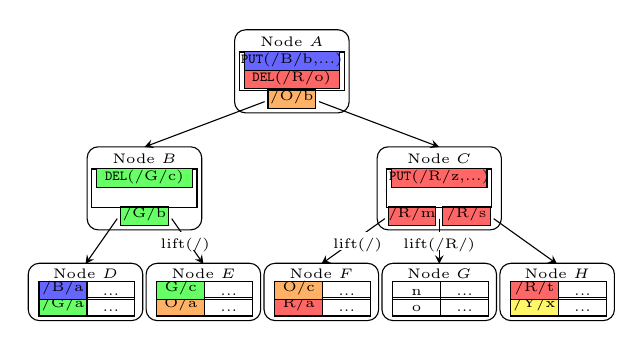
\begin{tikzpicture}[xscale=0.95, yscale=0.95]
            \node[anchor=south, rectangle, rounded corners, minimum height=.06\textwidth, minimum width=.12\textwidth, draw=black] at (0, 0) {};
            \node[anchor=south, font=\tiny] at (0, .036\textwidth) {Node $F$};
            \node[anchor=south, rectangle, minimum height=.015\textwidth, minimum width=.05\textwidth, draw=black, fill={red!60}] at (-.025\textwidth, .005\textwidth) {};
            \node[anchor=south, font=\tiny] at (-.025\textwidth, 0) {R/a};
            \node[anchor=south, rectangle, minimum height=.015\textwidth, minimum width=.05\textwidth, draw=black] at (.028\textwidth, .005\textwidth) {};
            \node[anchor=south, font=\tiny] at (.028\textwidth, 0) {...};
            \node[anchor=south, rectangle, minimum height=.015\textwidth, minimum width=.05\textwidth, draw=black, fill={orange!60}] at (-.025\textwidth, .023\textwidth) {};
            \node[anchor=south, font=\tiny] at (-.025\textwidth, .018\textwidth) {O/c};
            \node[anchor=south, rectangle, minimum height=.015\textwidth, minimum width=.05\textwidth, draw=black] at (.028\textwidth, .023\textwidth) {};
            \node[anchor=south, font=\tiny] at (.028\textwidth, .018\textwidth) {...};

            \node[anchor=south, rectangle, rounded corners, minimum height=.06\textwidth, minimum width=.12\textwidth, draw=black] at (.13\textwidth, 0) {};
            \node[anchor=south, font=\tiny] at (.13\textwidth, .036\textwidth) {Node $G$};
            \node[anchor=south, rectangle, minimum height=.015\textwidth, minimum width=.05\textwidth, draw=black] at (.105\textwidth, .005\textwidth) {};
            \node[anchor=south, font=\tiny] at (.105\textwidth, 0) {o};
            \node[anchor=south, rectangle, minimum height=.015\textwidth, minimum width=.05\textwidth, draw=black] at (.158\textwidth, .005\textwidth) {};
            \node[anchor=south, font=\tiny] at (.158\textwidth, 0) {...};
            \node[anchor=south, rectangle, minimum height=.015\textwidth, minimum width=.05\textwidth, draw=black] at (.105\textwidth, .023\textwidth) {};
            \node[anchor=south, font=\tiny] at (.105\textwidth, .018\textwidth) {n};
            \node[anchor=south, rectangle, minimum height=.015\textwidth, minimum width=.05\textwidth, draw=black] at (.158\textwidth, .023\textwidth) {};
            \node[anchor=south, font=\tiny] at (.158\textwidth, .018\textwidth) {...};

            \node[anchor=south, rectangle, rounded corners, minimum height=.06\textwidth, minimum width=.12\textwidth, draw=black] at (.26\textwidth, 0) {};
            \node[anchor=south, font=\tiny] at (.26\textwidth, .036\textwidth) {Node $H$};
            \node[anchor=south, rectangle, minimum height=.015\textwidth, minimum width=.05\textwidth, draw=black, fill={yellow!60}] at (.235\textwidth, .005\textwidth) {};
            \node[anchor=south, font=\tiny] at (.235\textwidth, 0) {/Y/x};
            \node[anchor=south, rectangle, minimum height=.015\textwidth, minimum width=.05\textwidth, draw=black] at (.288\textwidth, .005\textwidth) {};
            \node[anchor=south, font=\tiny] at (.288\textwidth, 0) {...};
            \node[anchor=south, rectangle, minimum height=.015\textwidth, minimum width=.05\textwidth, draw=black, fill={red!60}] at (.235\textwidth, .023\textwidth) {};
            \node[anchor=south, font=\tiny] at (.235\textwidth, .018\textwidth) {/R/t};
            \node[anchor=south, rectangle, minimum height=.015\textwidth, minimum width=.05\textwidth, draw=black] at (.288\textwidth, .023\textwidth) {};
            \node[anchor=south, font=\tiny] at (.288\textwidth, .018\textwidth) {...};

            \node[anchor=south, rectangle, rounded corners, minimum height=.06\textwidth, minimum width=.12\textwidth, draw=black] at (-.13\textwidth, 0) {};
            \node[anchor=south, font=\tiny] at (-.13\textwidth, .036\textwidth) {Node $E$};
            \node[anchor=south, rectangle, minimum height=.015\textwidth, minimum width=.05\textwidth, draw=black, fill={orange!60}] at (-.155\textwidth, .005\textwidth) {};
            \node[anchor=south, font=\tiny] at (-.155\textwidth, 0) {O/a};
            \node[anchor=south, rectangle, minimum height=.015\textwidth, minimum width=.05\textwidth, draw=black] at (-.102\textwidth, .005\textwidth) {};
            \node[anchor=south, font=\tiny] at (-.102\textwidth, 0) {...};
            \node[anchor=south, rectangle, minimum height=.015\textwidth, minimum width=.05\textwidth, draw=black, fill={green!60}] at (-.155\textwidth, .023\textwidth) {};
            \node[anchor=south, font=\tiny] at (-.155\textwidth, .018\textwidth) {G/c};
            \node[anchor=south, rectangle, minimum height=.015\textwidth, minimum width=.05\textwidth, draw=black] at (-.102\textwidth, .023\textwidth) {};
            \node[anchor=south, font=\tiny] at (-.102\textwidth, .018\textwidth) {...};

            \node[anchor=south, rectangle, rounded corners, minimum height=.06\textwidth, minimum width=.12\textwidth, draw=black] at (-.26\textwidth, 0) {};
            \node[anchor=south, font=\tiny] at (-.26\textwidth, .036\textwidth) {Node $D$};
            \node[anchor=south, rectangle, minimum height=.015\textwidth, minimum width=.05\textwidth, draw=black, fill={green!60}] at (-.285\textwidth, .005\textwidth) {};
            \node[anchor=south, font=\tiny] at (-.285\textwidth, 0) {/G/a};
            \node[anchor=south, rectangle, minimum height=.015\textwidth, minimum width=.05\textwidth, draw=black] at (-.232\textwidth, .005\textwidth) {};
            \node[anchor=south, font=\tiny] at (-.232\textwidth, 0) {...};
            \node[anchor=south, rectangle, minimum height=.015\textwidth, minimum width=.05\textwidth, draw=black, fill={blue!60}] at (-.285\textwidth, .023\textwidth) {};
            \node[anchor=south, font=\tiny] at (-.285\textwidth, .018\textwidth) {/B/a};
            \node[anchor=south, rectangle, minimum height=.015\textwidth, minimum width=.05\textwidth, draw=black] at (-.232\textwidth, .023\textwidth) {};
            \node[anchor=south, font=\tiny] at (-.232\textwidth, .018\textwidth) {...};

            \node[anchor=south, rectangle, rounded corners, minimum height=.087\textwidth, minimum width=.12\textwidth, draw=black] at (-.195\textwidth, .1\textwidth) {};
            \node[anchor=south, font=\tiny] at (-.195\textwidth, .163\textwidth) {Node $B$};
            \node[anchor=south, rectangle, minimum height=.015\textwidth, minimum width=.05\textwidth, draw=black, fill={green!60}] at (-.195\textwidth, .105\textwidth) {};
            \node[anchor=south, font=\tiny] at (-.195\textwidth, .1\textwidth) {/G/b};
            \node[anchor=south, rectangle, minimum height=.04\textwidth, minimum width=.11\textwidth, draw=black] at (-.195\textwidth, .125\textwidth) {};
            \node[anchor=south, rectangle, minimum height=.015\textwidth, minimum width=.1\textwidth, draw=black, fill={green!60}] at (-.195\textwidth, .147\textwidth) {};
            \node[anchor=south, font=\tiny] at  (-.195\textwidth, .141\textwidth) {\delm(/G/c)};

            \node[anchor=south, rectangle, rounded corners, minimum height=.087\textwidth, minimum width=.13\textwidth, draw=black] at (.13\textwidth, .1\textwidth) {};
            \node[anchor=south, font=\tiny] at (.13\textwidth, .163\textwidth) {Node $C$};
            \node[anchor=south, rectangle, minimum height=.015\textwidth, minimum width=.05\textwidth, draw=black, fill={red!60}] at (.1\textwidth, .105\textwidth) {};
            \node[anchor=south, font=\tiny] at (.1\textwidth, .1\textwidth) {/R/m};
            \node[anchor=south, rectangle, minimum height=.015\textwidth, minimum width=.05\textwidth, draw=black, fill={red!60}] at (.16\textwidth, .105\textwidth) {};
            \node[anchor=south, font=\tiny] at (.16\textwidth, .1\textwidth) {/R/s};
            \node[anchor=south, rectangle, minimum height=.04\textwidth, minimum width=.11\textwidth, draw=black] at (.13\textwidth, .125\textwidth) {};
            \node[anchor=south, rectangle, minimum height=.015\textwidth, minimum width=.1\textwidth, draw=black, fill={red!60}] at (.13\textwidth, .147\textwidth) {};
            \node[anchor=south, font=\tiny] at  (.13\textwidth, .141\textwidth) {\putm(/R/z,...)};

            \node[anchor=south, rectangle, rounded corners, minimum height=.087\textwidth, minimum width=.12\textwidth, draw=black] at (-.0325\textwidth, .229\textwidth) {};
            \node[anchor=south, font=\tiny] at (-.0325\textwidth, .292\textwidth) {Node $A$};
            \node[anchor=south, rectangle, minimum height=.015\textwidth, minimum width=.05\textwidth, draw=black, fill={orange!60}] at (-.0325\textwidth, .234\textwidth) {};
            \node[anchor=south, font=\tiny] at (-.0325\textwidth, .229\textwidth) {/O/b};
            \node[anchor=south, rectangle, minimum height=.04\textwidth, minimum width=.11\textwidth, draw=black] at (-.0325\textwidth, .254\textwidth) {};
            \node[anchor=south, rectangle, minimum height=.015\textwidth, minimum width=.1\textwidth, draw=black, fill={red!60}] at (-.0325\textwidth, .256\textwidth) {};
            \node[anchor=south, font=\tiny] at  (-.0325\textwidth, .25\textwidth) {\delm(/R/o)};
            \node[anchor=south, rectangle, minimum height=.015\textwidth, minimum width=.1\textwidth, draw=black, fill={blue!60}] at (-.0325\textwidth, .276\textwidth) {};
            \node[anchor=south, font=\tiny] at  (-.0325\textwidth, .27\textwidth) {\putm(/B/b,...)};

            \draw[->, >=stealth] (-.225\textwidth, .113\textwidth) -- (-.26\textwidth, .063\textwidth);
            \draw[->, >=stealth] (-.165\textwidth, .113\textwidth) -- (-.13\textwidth, .063\textwidth);
            \draw[->, >=stealth] (.13\textwidth, .113\textwidth) -- (.13\textwidth, .063\textwidth);
            \draw[->, >=stealth] (.19\textwidth, .113\textwidth) -- (.26\textwidth, .063\textwidth);
            \draw[->, >=stealth] (.07\textwidth, .113\textwidth) -- (0, .063\textwidth);
            \draw[->, >=stealth] (-.0625\textwidth, .242\textwidth) -- (-.195\textwidth, .192\textwidth);
            \draw[->, >=stealth] (-.0025\textwidth, .242\textwidth) -- (.13\textwidth, .192\textwidth);

            \node[anchor=north,rectangle, minimum height=.015\textwidth, minimum width=.05\textwidth, fill={white}] at (.13\textwidth, .099\textwidth) {};
            \node[anchor=north, font=\tiny] at (.13\textwidth, .102\textwidth) {lift(/R/)};
            \node[anchor=north,rectangle, minimum height=.015\textwidth, minimum width=.05\textwidth, fill={white}] at (.04\textwidth, .099\textwidth) {};
            \node[anchor=north, font=\tiny] at (.04\textwidth, .102\textwidth) {lift(/)};
            \node[anchor=north,rectangle, minimum height=.015\textwidth, minimum width=.05\textwidth, fill={white}] at (-.15\textwidth, .099\textwidth) {};
            \node[anchor=north, font=\tiny] at (-.15\textwidth, .102\textwidth) {lift(/)};
        \end{tikzpicture}
        \caption{\label{subfig:rc-1} The \bet before the range-clone operation.}
    \end{subfigure}
    \begin{subfigure}{\textwidth}
        \centering
        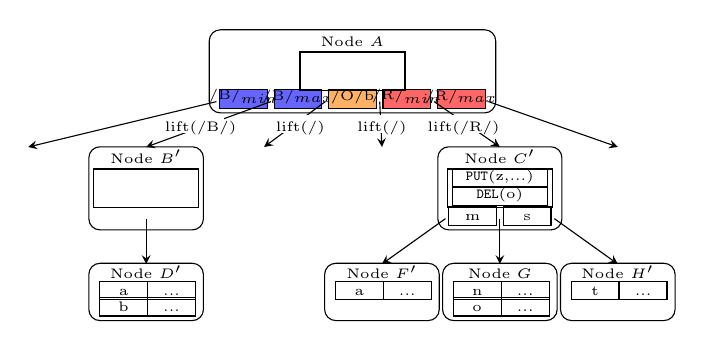
\begin{tikzpicture}[xscale=0.95, yscale=0.95]
            \node[anchor=south, rectangle, rounded corners, minimum height=.06\textwidth, minimum width=.12\textwidth, draw=black] at (0, 0) {};
            \node[anchor=south, font=\tiny] at (0, .036\textwidth) {Node $F'$};
            \node[anchor=south, rectangle, minimum height=.015\textwidth, minimum width=.05\textwidth, draw=black] at (-.025\textwidth, .023\textwidth) {};
            \node[anchor=south, font=\tiny] at (-.025\textwidth, .018\textwidth) {a};
            \node[anchor=south, rectangle, minimum height=.015\textwidth, minimum width=.05\textwidth, draw=black] at (.028\textwidth, .023\textwidth) {};
            \node[anchor=south, font=\tiny] at (.028\textwidth, .018\textwidth) {...};

            \node[anchor=south, rectangle, rounded corners, minimum height=.06\textwidth, minimum width=.12\textwidth, draw=black] at (.13\textwidth, 0) {};
            \node[anchor=south, font=\tiny] at (.13\textwidth, .036\textwidth) {Node $G$};
            \node[anchor=south, rectangle, minimum height=.015\textwidth, minimum width=.05\textwidth, draw=black] at (.105\textwidth, .005\textwidth) {};
            \node[anchor=south, font=\tiny] at (.105\textwidth, 0) {o};
            \node[anchor=south, rectangle, minimum height=.015\textwidth, minimum width=.05\textwidth, draw=black] at (.158\textwidth, .005\textwidth) {};
            \node[anchor=south, font=\tiny] at (.158\textwidth, 0) {...};
            \node[anchor=south, rectangle, minimum height=.015\textwidth, minimum width=.05\textwidth, draw=black] at (.105\textwidth, .023\textwidth) {};
            \node[anchor=south, font=\tiny] at (.105\textwidth, .018\textwidth) {n};
            \node[anchor=south, rectangle, minimum height=.015\textwidth, minimum width=.05\textwidth, draw=black] at (.158\textwidth, .023\textwidth) {};
            \node[anchor=south, font=\tiny] at (.158\textwidth, .018\textwidth) {...};

            \node[anchor=south, rectangle, rounded corners, minimum height=.06\textwidth, minimum width=.12\textwidth, draw=black] at (.26\textwidth, 0) {};
            \node[anchor=south, font=\tiny] at (.26\textwidth, .036\textwidth) {Node $H'$};
            \node[anchor=south, rectangle, minimum height=.015\textwidth, minimum width=.05\textwidth, draw=black] at (.235\textwidth, .023\textwidth) {};
            \node[anchor=south, font=\tiny] at (.235\textwidth, .018\textwidth) {t};
            \node[anchor=south, rectangle, minimum height=.015\textwidth, minimum width=.05\textwidth, draw=black] at (.288\textwidth, .023\textwidth) {};
            \node[anchor=south, font=\tiny] at (.288\textwidth, .018\textwidth) {...};

            \node[anchor=south, rectangle, rounded corners, minimum height=.06\textwidth, minimum width=.12\textwidth, draw=black] at (-.26\textwidth, 0) {};
            \node[anchor=south, font=\tiny] at (-.26\textwidth, .036\textwidth) {Node $D'$};
            \node[anchor=south, rectangle, minimum height=.015\textwidth, minimum width=.05\textwidth, draw=black] at (-.285\textwidth, .005\textwidth) {};
            \node[anchor=south, font=\tiny] at (-.285\textwidth, 0) {b};
            \node[anchor=south, rectangle, minimum height=.015\textwidth, minimum width=.05\textwidth, draw=black] at (-.232\textwidth, .005\textwidth) {};
            \node[anchor=south, font=\tiny] at (-.232\textwidth, 0) {...};
            \node[anchor=south, rectangle, minimum height=.015\textwidth, minimum width=.05\textwidth, draw=black] at (-.285\textwidth, .023\textwidth) {};
            \node[anchor=south, font=\tiny] at (-.285\textwidth, .018\textwidth) {a};
            \node[anchor=south, rectangle, minimum height=.015\textwidth, minimum width=.05\textwidth, draw=black] at (-.232\textwidth, .023\textwidth) {};
            \node[anchor=south, font=\tiny] at (-.232\textwidth, .018\textwidth) {...};

            \node[anchor=south, rectangle, rounded corners, minimum height=.087\textwidth, minimum width=.12\textwidth, draw=black] at (-.26\textwidth, .1\textwidth) {};
            \node[anchor=south, font=\tiny] at (-.26\textwidth, .163\textwidth) {Node $B'$};
            \node[anchor=south, rectangle, minimum height=.04\textwidth, minimum width=.11\textwidth, draw=black] at (-.26\textwidth, .125\textwidth) {};

            \node[anchor=south, rectangle, rounded corners, minimum height=.087\textwidth, minimum width=.13\textwidth, draw=black] at (.13\textwidth, .1\textwidth) {};
            \node[anchor=south, font=\tiny] at (.13\textwidth, .163\textwidth) {Node $C'$};
            \node[anchor=south, rectangle, minimum height=.015\textwidth, minimum width=.05\textwidth, draw=black] at (.1\textwidth, .105\textwidth) {};
            \node[anchor=south, font=\tiny] at (.1\textwidth, .1\textwidth) {m};
            \node[anchor=south, rectangle, minimum height=.015\textwidth, minimum width=.05\textwidth, draw=black] at (.16\textwidth, .105\textwidth) {};
            \node[anchor=south, font=\tiny] at (.16\textwidth, .1\textwidth) {s};
            \node[anchor=south, rectangle, minimum height=.04\textwidth, minimum width=.11\textwidth, draw=black] at (.13\textwidth, .125\textwidth) {};
            \node[anchor=south, rectangle, minimum height=.015\textwidth, minimum width=.1\textwidth, draw=black] at (.13\textwidth, .147\textwidth) {};
            \node[anchor=south, font=\tiny] at  (.13\textwidth, .141\textwidth) {\putm(z,...)};
            \node[anchor=south, rectangle, minimum height=.015\textwidth, minimum width=.1\textwidth, draw=black] at (.13\textwidth, .127\textwidth) {};
            \node[anchor=south, font=\tiny] at  (.13\textwidth, .121\textwidth) {\delm(o)};

            \node[anchor=south, rectangle, rounded corners, minimum height=.087\textwidth, minimum width=.3\textwidth, draw=black] at (-.0325\textwidth, .229\textwidth) {};
            \node[anchor=south, font=\tiny] at (-.0325\textwidth, .292\textwidth) {Node $A$};
            \node[anchor=south, rectangle, minimum height=.015\textwidth, minimum width=.05\textwidth, draw=black, fill={blue!60}] at (-.1525\textwidth, .234\textwidth) {};
            \node[anchor=south, font=\tiny] at (-.1525\textwidth, .229\textwidth) {/B/$_{min}$};
            \node[anchor=south, rectangle, minimum height=.015\textwidth, minimum width=.05\textwidth, draw=black, fill={blue!60}] at (-.0925\textwidth, .234\textwidth) {};
            \node[anchor=south, font=\tiny] at (-.0925\textwidth, .229\textwidth) {/B/$_{max}$};
            \node[anchor=south, rectangle, minimum height=.015\textwidth, minimum width=.05\textwidth, draw=black, fill={orange!60}] at (-.0325\textwidth, .234\textwidth) {};
            \node[anchor=south, font=\tiny] at (-.0325\textwidth, .229\textwidth) {/O/b};
            \node[anchor=south, rectangle, minimum height=.015\textwidth, minimum width=.05\textwidth, draw=black, fill={red!60}] at (.0275\textwidth, .234\textwidth) {};
            \node[anchor=south, font=\tiny] at (.0275\textwidth, .229\textwidth) {/R/$_{min}$};
            \node[anchor=south, rectangle, minimum height=.015\textwidth, minimum width=.05\textwidth, draw=black, fill={red!60}] at (.0875\textwidth, .234\textwidth) {};
            \node[anchor=south, font=\tiny] at (.0875\textwidth, .229\textwidth) {/R/$_{max}$};
            \node[anchor=south, rectangle, minimum height=.04\textwidth, minimum width=.11\textwidth, draw=black] at (-.0325\textwidth, .254\textwidth) {};

            \draw[->, >=stealth] (-.26\textwidth, .113\textwidth) -- (-.26\textwidth, .063\textwidth);
            \draw[->, >=stealth] (.13\textwidth, .113\textwidth) -- (.13\textwidth, .063\textwidth);
            \draw[->, >=stealth] (.19\textwidth, .113\textwidth) -- (.26\textwidth, .063\textwidth);
            \draw[->, >=stealth] (.07\textwidth, .113\textwidth) -- (0, .063\textwidth);
            \draw[->, >=stealth] (-.1825\textwidth, .242\textwidth) -- (-.39\textwidth, .192\textwidth);
            \draw[->, >=stealth] (-.1225\textwidth, .242\textwidth) -- (-.26\textwidth, .192\textwidth);
            \draw[->, >=stealth] (-.0625\textwidth, .242\textwidth) -- (-.13\textwidth, .192\textwidth);
            \draw[->, >=stealth] (-.0025\textwidth, .242\textwidth) -- (0, .192\textwidth);
            \draw[->, >=stealth] (.0575\textwidth, .242\textwidth) -- (.13\textwidth, .192\textwidth);
            \draw[->, >=stealth] (.1175\textwidth, .242\textwidth) -- (.26\textwidth, .192\textwidth);

            \node[anchor=north,rectangle, minimum height=.015\textwidth, minimum width=.05\textwidth, fill={white}] at (-.20\textwidth, .228\textwidth) {};
            \node[anchor=north, font=\tiny] at (-.20\textwidth, .231\textwidth) {lift(/B/)};
            \node[anchor=north,rectangle, minimum height=.015\textwidth, minimum width=.05\textwidth, fill={white}] at (-.09\textwidth, .228\textwidth) {};
            \node[anchor=north, font=\tiny] at (-.09\textwidth, .231\textwidth) {lift(/)};
            \node[anchor=north,rectangle, minimum height=.015\textwidth, minimum width=.05\textwidth, fill={white}] at (0, .228\textwidth) {};
            \node[anchor=north, font=\tiny] at (0, .231\textwidth) {lift(/)};
            \node[anchor=north,rectangle, minimum height=.015\textwidth, minimum width=.05\textwidth, fill={white}] at (.09\textwidth, .228\textwidth) {};
            \node[anchor=north, font=\tiny] at (.09\textwidth, .231\textwidth) {lift(/R/)};
        \end{tikzpicture}
        \caption{\label{subfig:rc-2} The range-clone operation slices out the
            source and destination subtrees.}
    \end{subfigure}
    \begin{subfigure}{\textwidth}
        \centering
        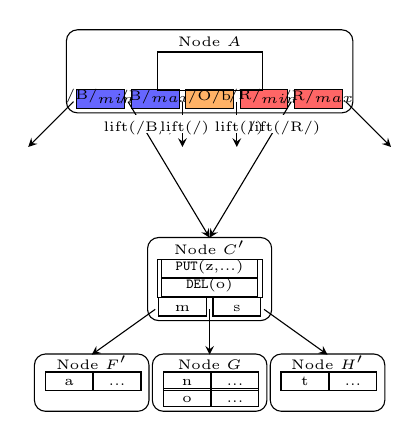
\begin{tikzpicture}[xscale=0.95, yscale=0.95]
            \node[anchor=south, rectangle, rounded corners, minimum height=.06\textwidth, minimum width=.12\textwidth, draw=black] at (-.1625\textwidth, -.1\textwidth) {};
            \node[anchor=south, font=\tiny] at (-.1625\textwidth, -.064\textwidth) {Node $F'$};
            \node[anchor=south, rectangle, minimum height=.015\textwidth, minimum width=.05\textwidth, draw=black] at (-.1875\textwidth, -.077\textwidth) {};
            \node[anchor=south, font=\tiny] at (-.1875\textwidth, -.082\textwidth) {a};
            \node[anchor=south, rectangle, minimum height=.015\textwidth, minimum width=.05\textwidth, draw=black] at (-.1345\textwidth, -.077\textwidth) {};
            \node[anchor=south, font=\tiny] at (-.1345\textwidth, -.082\textwidth) {...};

            \node[anchor=south, rectangle, rounded corners, minimum height=.06\textwidth, minimum width=.12\textwidth, draw=black] at (-.0325\textwidth, -.1\textwidth) {};
            \node[anchor=south, font=\tiny] at (-.0325\textwidth, -.064\textwidth) {Node $G$};
            \node[anchor=south, rectangle, minimum height=.015\textwidth, minimum width=.05\textwidth, draw=black] at (-.0575\textwidth, -.095\textwidth) {};
            \node[anchor=south, font=\tiny] at (-.0575\textwidth, -.1\textwidth) {o};
            \node[anchor=south, rectangle, minimum height=.015\textwidth, minimum width=.05\textwidth, draw=black] at (-.0045\textwidth, -.095\textwidth) {};
            \node[anchor=south, font=\tiny] at (-.0045\textwidth, -.1\textwidth) {...};
            \node[anchor=south, rectangle, minimum height=.015\textwidth, minimum width=.05\textwidth, draw=black] at (-.0575\textwidth, -.077\textwidth) {};
            \node[anchor=south, font=\tiny] at (-.0575\textwidth, -.082\textwidth) {n};
            \node[anchor=south, rectangle, minimum height=.015\textwidth, minimum width=.05\textwidth, draw=black] at (-.0045\textwidth, -.077\textwidth) {};
            \node[anchor=south, font=\tiny] at (-.0045\textwidth, -.082\textwidth) {...};

            \node[anchor=south, rectangle, rounded corners, minimum height=.06\textwidth, minimum width=.12\textwidth, draw=black] at (.0975\textwidth, -.1\textwidth) {};
            \node[anchor=south, font=\tiny] at (.0975\textwidth, -.064\textwidth) {Node $H'$};
            \node[anchor=south, rectangle, minimum height=.015\textwidth, minimum width=.05\textwidth, draw=black] at (.0725\textwidth, -.077\textwidth) {};
            \node[anchor=south, font=\tiny] at (.0725\textwidth, -.082\textwidth) {t};
            \node[anchor=south, rectangle, minimum height=.015\textwidth, minimum width=.05\textwidth, draw=black] at (.1255\textwidth, -.077\textwidth) {};
            \node[anchor=south, font=\tiny] at (.1255\textwidth, -.082\textwidth) {...};

            \node[anchor=south, rectangle, rounded corners, minimum height=.087\textwidth, minimum width=.13\textwidth, draw=black] at (-.0325\textwidth, 0) {};
            \node[anchor=south, font=\tiny] at (-.0325\textwidth, .063\textwidth) {Node $C'$};
            \node[anchor=south, rectangle, minimum height=.015\textwidth, minimum width=.05\textwidth, draw=black] at (-.0625\textwidth, .005\textwidth) {};
            \node[anchor=south, font=\tiny] at (-.0625\textwidth, 0) {m};
            \node[anchor=south, rectangle, minimum height=.015\textwidth, minimum width=.05\textwidth, draw=black] at (-.0025\textwidth, .005\textwidth) {};
            \node[anchor=south, font=\tiny] at (-.0025\textwidth, 0) {s};
            \node[anchor=south, rectangle, minimum height=.04\textwidth, minimum width=.11\textwidth, draw=black] at (-.0325\textwidth, .025\textwidth) {};
            \node[anchor=south, rectangle, minimum height=.015\textwidth, minimum width=.1\textwidth, draw=black] at (-.0325\textwidth, .047\textwidth) {};
            \node[anchor=south, font=\tiny] at  (-.0325\textwidth, .041\textwidth) {\putm(z,...)};
            \node[anchor=south, rectangle, minimum height=.015\textwidth, minimum width=.1\textwidth, draw=black] at (-.0325\textwidth, .027\textwidth) {};
            \node[anchor=south, font=\tiny] at  (-.0325\textwidth, .021\textwidth) {\delm(o)};

            \node[anchor=south, rectangle, rounded corners, minimum height=.087\textwidth, minimum width=.3\textwidth, draw=black] at (-.0325\textwidth, .229\textwidth) {};
            \node[anchor=south, font=\tiny] at (-.0325\textwidth, .292\textwidth) {Node $A$};
            \node[anchor=south, rectangle, minimum height=.015\textwidth, minimum width=.05\textwidth, draw=black, fill={blue!60}] at (-.1525\textwidth, .234\textwidth) {};
            \node[anchor=south, font=\tiny] at (-.1525\textwidth, .229\textwidth) {/B/$_{min}$};
            \node[anchor=south, rectangle, minimum height=.015\textwidth, minimum width=.05\textwidth, draw=black, fill={blue!60}] at (-.0925\textwidth, .234\textwidth) {};
            \node[anchor=south, font=\tiny] at (-.0925\textwidth, .229\textwidth) {/B/$_{max}$};
            \node[anchor=south, rectangle, minimum height=.015\textwidth, minimum width=.05\textwidth, draw=black, fill={orange!60}] at (-.0325\textwidth, .234\textwidth) {};
            \node[anchor=south, font=\tiny] at (-.0325\textwidth, .229\textwidth) {/O/b};
            \node[anchor=south, rectangle, minimum height=.015\textwidth, minimum width=.05\textwidth, draw=black, fill={red!60}] at (.0275\textwidth, .234\textwidth) {};
            \node[anchor=south, font=\tiny] at (.0275\textwidth, .229\textwidth) {/R/$_{min}$};
            \node[anchor=south, rectangle, minimum height=.015\textwidth, minimum width=.05\textwidth, draw=black, fill={red!60}] at (.0875\textwidth, .234\textwidth) {};
            \node[anchor=south, font=\tiny] at (.0875\textwidth, .229\textwidth) {/R/$_{max}$};
            \node[anchor=south, rectangle, minimum height=.04\textwidth, minimum width=.11\textwidth, draw=black] at (-.0325\textwidth, .254\textwidth) {};

            \draw[->, >=stealth] (-.0325\textwidth, .013\textwidth) -- (-.0325\textwidth, -.037\textwidth);
            \draw[->, >=stealth] (.0275\textwidth, .013\textwidth) -- (.0975\textwidth, -.037\textwidth);
            \draw[->, >=stealth] (-.0925\textwidth, .013\textwidth) -- (-.1625\textwidth, -.037\textwidth);
            \draw[->, >=stealth] (-.1825\textwidth, .242\textwidth) -- (-.2325\textwidth, .192\textwidth);
            \draw[->, >=stealth] (-.1225\textwidth, .242\textwidth) -- (-.0325\textwidth, .092\textwidth);
            \draw[->, >=stealth] (-.0625\textwidth, .242\textwidth) -- (-.0625\textwidth, .192\textwidth);
            \draw[->, >=stealth] (-.0025\textwidth, .242\textwidth) -- (-.0025\textwidth, .192\textwidth);
            \draw[->, >=stealth] (.0575\textwidth, .242\textwidth) -- (-.0325\textwidth, .092\textwidth);
            \draw[->, >=stealth] (.1175\textwidth, .242\textwidth) -- (.1675\textwidth, .192\textwidth);

            \node[anchor=north,rectangle, minimum height=.015\textwidth, minimum width=.05\textwidth, fill={white}] at (-.11\textwidth, .228\textwidth) {};
            \node[anchor=north, font=\tiny] at (-.11\textwidth, .231\textwidth) {lift(/B/)};
            \node[anchor=north,rectangle, minimum height=.015\textwidth, minimum width=.05\textwidth, fill={white}] at (-.06\textwidth, .228\textwidth) {};
            \node[anchor=north, font=\tiny] at (-.06\textwidth, .231\textwidth) {lift(/)};
            \node[anchor=north,rectangle, minimum height=.015\textwidth, minimum width=.05\textwidth, fill={white}] at (0, .228\textwidth) {};
            \node[anchor=north, font=\tiny] at (0, .231\textwidth) {lift(/)};
            \node[anchor=north,rectangle, minimum height=.015\textwidth, minimum width=.05\textwidth, fill={white}] at (.05\textwidth, .228\textwidth) {};
            \node[anchor=north, font=\tiny] at (.05\textwidth, .231\textwidth) {lift(/R/)};
        \end{tikzpicture}
        \caption{\label{subfig:rc-3} The range-clone operations shares the source
            subtree at both source and destination and garbage-collects the
            destination subtree.}
    \end{subfigure}
    \caption[All operations in range-clone]{\label{fig:rc}
        All operations needed in range-clone(``/R/'', ``/B/'').}
\end{figure}

The range-clone operation can be done on \bets by slightly modifying the
range-rename operation.
In particular, after slicing out the source and destination subtrees with tree
surgery,
instead of swapping the two subtrees and injecting a range-delete message
for source keys in a range-rename operation,
a range-clone operation can share the source subtree in both source and
destination and garbage-collects the destination subtree.

Figure~\ref{fig:rc} shows an example of performing the work of
range-clone(``/R/'', ``/B/'') on the lifted \bet in Figure~\ref{subfig:rc-1}.
Figure~\ref{subfig:rc-2} shows the lifted \bet after tree surgery.
Tree surgery slices out the source and destination subtree, which is identical
to that in range-rename.
In Figure~\ref{subfig:rc-3}, the lifted \bet garbage-collects the destination
subtree, rooted at Node $B'$, and sets the parent-to-child pointer between
``/B/$_{min}$'' and ``/B/$_{max}$'' to Node $C'$,
the root node of the source subtree.

Range-rename transforms a lifted \bet into a lifted \bedag
(Directed Acyclic Graph) with some constraints.
Because the \bedag is generated by sharing subtrees in a \bet,
there is still one root node in the \bedag,
which can reach all nodes in the \bedag through parent-to-child pointers.
And since the source and destination subtrees generated by tree surgery are at
the same height, the length of any root-to-leaf path in the \bedag is still
logarithmic in the size of the graph.

In a lifted \bedag, the root-to-leaf traversals of different queries may end up
reaching the same leaf node, fetching the same key/value pair.
However, because key lifting requires queries to reconstruct the full key by
concatenating lifted prefixes, different queries are able to see different keys.
For example, in Figure~\ref{subfig:rc-3}, queries for key ``/R/n'' and ``/B/n''
follow the same root-to-leaf path and get the same key/value pair from the
leaf node, Node $G$.
However, because two queries follow different parent-to-child pointers with
different lifted prefixes fromNode $A$ to Node $C'$,
they view the key/value pair with different prefixes.

\begin{figure}
    \begin{subfigure}{\textwidth}
        \centering
        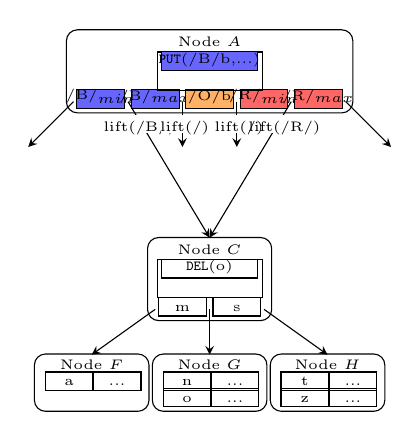
\begin{tikzpicture}[xscale=0.95, yscale=0.95]
            \node[anchor=south, rectangle, rounded corners, minimum height=.06\textwidth, minimum width=.12\textwidth, draw=black] at (-.1625\textwidth, -.1\textwidth) {};
            \node[anchor=south, font=\tiny] at (-.1625\textwidth, -.064\textwidth) {Node $F$};
            \node[anchor=south, rectangle, minimum height=.015\textwidth, minimum width=.05\textwidth, draw=black] at (-.1875\textwidth, -.077\textwidth) {};
            \node[anchor=south, font=\tiny] at (-.1875\textwidth, -.082\textwidth) {a};
            \node[anchor=south, rectangle, minimum height=.015\textwidth, minimum width=.05\textwidth, draw=black] at (-.1345\textwidth, -.077\textwidth) {};
            \node[anchor=south, font=\tiny] at (-.1345\textwidth, -.082\textwidth) {...};

            \node[anchor=south, rectangle, rounded corners, minimum height=.06\textwidth, minimum width=.12\textwidth, draw=black] at (-.0325\textwidth, -.1\textwidth) {};
            \node[anchor=south, font=\tiny] at (-.0325\textwidth, -.064\textwidth) {Node $G$};
            \node[anchor=south, rectangle, minimum height=.015\textwidth, minimum width=.05\textwidth, draw=black] at (-.0575\textwidth, -.095\textwidth) {};
            \node[anchor=south, font=\tiny] at (-.0575\textwidth, -.1\textwidth) {o};
            \node[anchor=south, rectangle, minimum height=.015\textwidth, minimum width=.05\textwidth, draw=black] at (-.0045\textwidth, -.095\textwidth) {};
            \node[anchor=south, font=\tiny] at (-.0045\textwidth, -.1\textwidth) {...};
            \node[anchor=south, rectangle, minimum height=.015\textwidth, minimum width=.05\textwidth, draw=black] at (-.0575\textwidth, -.077\textwidth) {};
            \node[anchor=south, font=\tiny] at (-.0575\textwidth, -.082\textwidth) {n};
            \node[anchor=south, rectangle, minimum height=.015\textwidth, minimum width=.05\textwidth, draw=black] at (-.0045\textwidth, -.077\textwidth) {};
            \node[anchor=south, font=\tiny] at (-.0045\textwidth, -.082\textwidth) {...};

            \node[anchor=south, rectangle, rounded corners, minimum height=.06\textwidth, minimum width=.12\textwidth, draw=black] at (.0975\textwidth, -.1\textwidth) {};
            \node[anchor=south, font=\tiny] at (.0975\textwidth, -.064\textwidth) {Node $H$};
            \node[anchor=south, rectangle, minimum height=.015\textwidth, minimum width=.05\textwidth, draw=black] at (.0725\textwidth, -.095\textwidth) {};
            \node[anchor=south, font=\tiny] at (.0725\textwidth, -.1\textwidth) {z};
            \node[anchor=south, rectangle, minimum height=.015\textwidth, minimum width=.05\textwidth, draw=black] at (.1255\textwidth, -.095\textwidth) {};
            \node[anchor=south, font=\tiny] at (.1255\textwidth, -.1\textwidth) {...};
            \node[anchor=south, rectangle, minimum height=.015\textwidth, minimum width=.05\textwidth, draw=black] at (.0725\textwidth, -.077\textwidth) {};
            \node[anchor=south, font=\tiny] at (.0725\textwidth, -.082\textwidth) {t};
            \node[anchor=south, rectangle, minimum height=.015\textwidth, minimum width=.05\textwidth, draw=black] at (.1255\textwidth, -.077\textwidth) {};
            \node[anchor=south, font=\tiny] at (.1255\textwidth, -.082\textwidth) {...};

            \node[anchor=south, rectangle, rounded corners, minimum height=.087\textwidth, minimum width=.13\textwidth, draw=black] at (-.0325\textwidth, 0) {};
            \node[anchor=south, font=\tiny] at (-.0325\textwidth, .063\textwidth) {Node $C$};
            \node[anchor=south, rectangle, minimum height=.015\textwidth, minimum width=.05\textwidth, draw=black] at (-.0625\textwidth, .005\textwidth) {};
            \node[anchor=south, font=\tiny] at (-.0625\textwidth, 0) {m};
            \node[anchor=south, rectangle, minimum height=.015\textwidth, minimum width=.05\textwidth, draw=black] at (-.0025\textwidth, .005\textwidth) {};
            \node[anchor=south, font=\tiny] at (-.0025\textwidth, 0) {s};
            \node[anchor=south, rectangle, minimum height=.04\textwidth, minimum width=.11\textwidth, draw=black] at (-.0325\textwidth, .025\textwidth) {};
            \node[anchor=south, rectangle, minimum height=.015\textwidth, minimum width=.1\textwidth, draw=black] at (-.0325\textwidth, .047\textwidth) {};
            \node[anchor=south, font=\tiny] at  (-.0325\textwidth, .041\textwidth) {\delm(o)};

            \node[anchor=south, rectangle, rounded corners, minimum height=.087\textwidth, minimum width=.3\textwidth, draw=black] at (-.0325\textwidth, .229\textwidth) {};
            \node[anchor=south, font=\tiny] at (-.0325\textwidth, .292\textwidth) {Node $A$};
            \node[anchor=south, rectangle, minimum height=.015\textwidth, minimum width=.05\textwidth, draw=black, fill={blue!60}] at (-.1525\textwidth, .234\textwidth) {};
            \node[anchor=south, font=\tiny] at (-.1525\textwidth, .229\textwidth) {/B/$_{min}$};
            \node[anchor=south, rectangle, minimum height=.015\textwidth, minimum width=.05\textwidth, draw=black, fill={blue!60}] at (-.0925\textwidth, .234\textwidth) {};
            \node[anchor=south, font=\tiny] at (-.0925\textwidth, .229\textwidth) {/B/$_{max}$};
            \node[anchor=south, rectangle, minimum height=.015\textwidth, minimum width=.05\textwidth, draw=black, fill={orange!60}] at (-.0325\textwidth, .234\textwidth) {};
            \node[anchor=south, font=\tiny] at (-.0325\textwidth, .229\textwidth) {/O/b};
            \node[anchor=south, rectangle, minimum height=.015\textwidth, minimum width=.05\textwidth, draw=black, fill={red!60}] at (.0275\textwidth, .234\textwidth) {};
            \node[anchor=south, font=\tiny] at (.0275\textwidth, .229\textwidth) {/R/$_{min}$};
            \node[anchor=south, rectangle, minimum height=.015\textwidth, minimum width=.05\textwidth, draw=black, fill={red!60}] at (.0875\textwidth, .234\textwidth) {};
            \node[anchor=south, font=\tiny] at (.0875\textwidth, .229\textwidth) {/R/$_{max}$};
            \node[anchor=south, rectangle, minimum height=.04\textwidth, minimum width=.11\textwidth, draw=black] at (-.0325\textwidth, .254\textwidth) {};
            \node[anchor=south, rectangle, minimum height=.015\textwidth, minimum width=.1\textwidth, draw=black, fill={blue!60}] at (-.0325\textwidth, .276\textwidth) {};
            \node[anchor=south, font=\tiny] at  (-.0325\textwidth, .27\textwidth) {\putm(/B/b,...)};

            \draw[->, >=stealth] (-.0325\textwidth, .013\textwidth) -- (-.0325\textwidth, -.037\textwidth);
            \draw[->, >=stealth] (.0275\textwidth, .013\textwidth) -- (.0975\textwidth, -.037\textwidth);
            \draw[->, >=stealth] (-.0925\textwidth, .013\textwidth) -- (-.1625\textwidth, -.037\textwidth);
            \draw[->, >=stealth] (-.1825\textwidth, .242\textwidth) -- (-.2325\textwidth, .192\textwidth);
            \draw[->, >=stealth] (-.1225\textwidth, .242\textwidth) -- (-.0325\textwidth, .092\textwidth);
            \draw[->, >=stealth] (-.0625\textwidth, .242\textwidth) -- (-.0625\textwidth, .192\textwidth);
            \draw[->, >=stealth] (-.0025\textwidth, .242\textwidth) -- (-.0025\textwidth, .192\textwidth);
            \draw[->, >=stealth] (.0575\textwidth, .242\textwidth) -- (-.0325\textwidth, .092\textwidth);
            \draw[->, >=stealth] (.1175\textwidth, .242\textwidth) -- (.1675\textwidth, .192\textwidth);

            \node[anchor=north,rectangle, minimum height=.015\textwidth, minimum width=.05\textwidth, fill={white}] at (-.11\textwidth, .228\textwidth) {};
            \node[anchor=north, font=\tiny] at (-.11\textwidth, .231\textwidth) {lift(/B/)};
            \node[anchor=north,rectangle, minimum height=.015\textwidth, minimum width=.05\textwidth, fill={white}] at (-.06\textwidth, .228\textwidth) {};
            \node[anchor=north, font=\tiny] at (-.06\textwidth, .231\textwidth) {lift(/)};
            \node[anchor=north,rectangle, minimum height=.015\textwidth, minimum width=.05\textwidth, fill={white}] at (0, .228\textwidth) {};
            \node[anchor=north, font=\tiny] at (0, .231\textwidth) {lift(/)};
            \node[anchor=north,rectangle, minimum height=.015\textwidth, minimum width=.05\textwidth, fill={white}] at (.05\textwidth, .228\textwidth) {};
            \node[anchor=north, font=\tiny] at (.05\textwidth, .231\textwidth) {lift(/R/)};
        \end{tikzpicture}
        \caption{\label{subfig:cow-1} Node $C$ is a shared by two
            parent-to-child pointers in Node $A$.}
    \end{subfigure}
    \begin{subfigure}{\textwidth}
        \centering
        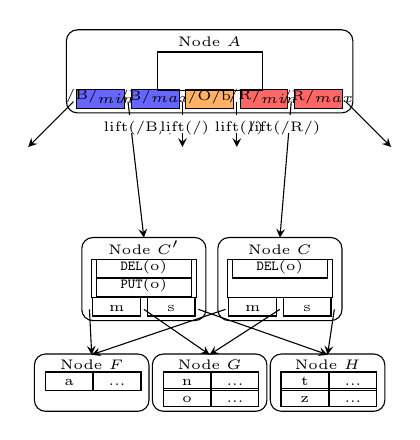
\begin{tikzpicture}[xscale=0.95, yscale=0.95]
            \node[anchor=south, rectangle, rounded corners, minimum height=.06\textwidth, minimum width=.12\textwidth, draw=black] at (-.1625\textwidth, -.1\textwidth) {};
            \node[anchor=south, font=\tiny] at (-.1625\textwidth, -.064\textwidth) {Node $F$};
            \node[anchor=south, rectangle, minimum height=.015\textwidth, minimum width=.05\textwidth, draw=black] at (-.1875\textwidth, -.077\textwidth) {};
            \node[anchor=south, font=\tiny] at (-.1875\textwidth, -.082\textwidth) {a};
            \node[anchor=south, rectangle, minimum height=.015\textwidth, minimum width=.05\textwidth, draw=black] at (-.1345\textwidth, -.077\textwidth) {};
            \node[anchor=south, font=\tiny] at (-.1345\textwidth, -.082\textwidth) {...};

            \node[anchor=south, rectangle, rounded corners, minimum height=.06\textwidth, minimum width=.12\textwidth, draw=black] at (-.0325\textwidth, -.1\textwidth) {};
            \node[anchor=south, font=\tiny] at (-.0325\textwidth, -.064\textwidth) {Node $G$};
            \node[anchor=south, rectangle, minimum height=.015\textwidth, minimum width=.05\textwidth, draw=black] at (-.0575\textwidth, -.095\textwidth) {};
            \node[anchor=south, font=\tiny] at (-.0575\textwidth, -.1\textwidth) {o};
            \node[anchor=south, rectangle, minimum height=.015\textwidth, minimum width=.05\textwidth, draw=black] at (-.0045\textwidth, -.095\textwidth) {};
            \node[anchor=south, font=\tiny] at (-.0045\textwidth, -.1\textwidth) {...};
            \node[anchor=south, rectangle, minimum height=.015\textwidth, minimum width=.05\textwidth, draw=black] at (-.0575\textwidth, -.077\textwidth) {};
            \node[anchor=south, font=\tiny] at (-.0575\textwidth, -.082\textwidth) {n};
            \node[anchor=south, rectangle, minimum height=.015\textwidth, minimum width=.05\textwidth, draw=black] at (-.0045\textwidth, -.077\textwidth) {};
            \node[anchor=south, font=\tiny] at (-.0045\textwidth, -.082\textwidth) {...};

            \node[anchor=south, rectangle, rounded corners, minimum height=.06\textwidth, minimum width=.12\textwidth, draw=black] at (.0975\textwidth, -.1\textwidth) {};
            \node[anchor=south, font=\tiny] at (.0975\textwidth, -.064\textwidth) {Node $H$};
            \node[anchor=south, rectangle, minimum height=.015\textwidth, minimum width=.05\textwidth, draw=black] at (.0725\textwidth, -.095\textwidth) {};
            \node[anchor=south, font=\tiny] at (.0725\textwidth, -.1\textwidth) {z};
            \node[anchor=south, rectangle, minimum height=.015\textwidth, minimum width=.05\textwidth, draw=black] at (.1255\textwidth, -.095\textwidth) {};
            \node[anchor=south, font=\tiny] at (.1255\textwidth, -.1\textwidth) {...};
            \node[anchor=south, rectangle, minimum height=.015\textwidth, minimum width=.05\textwidth, draw=black] at (.0725\textwidth, -.077\textwidth) {};
            \node[anchor=south, font=\tiny] at (.0725\textwidth, -.082\textwidth) {t};
            \node[anchor=south, rectangle, minimum height=.015\textwidth, minimum width=.05\textwidth, draw=black] at (.1255\textwidth, -.077\textwidth) {};
            \node[anchor=south, font=\tiny] at (.1255\textwidth, -.082\textwidth) {...};

            \node[anchor=south, rectangle, rounded corners, minimum height=.087\textwidth, minimum width=.13\textwidth, draw=black] at (.045\textwidth, 0) {};
            \node[anchor=south, font=\tiny] at (.045\textwidth, .063\textwidth) {Node $C$};
            \node[anchor=south, rectangle, minimum height=.015\textwidth, minimum width=.05\textwidth, draw=black] at (.015\textwidth, .005\textwidth) {};
            \node[anchor=south, font=\tiny] at (.015\textwidth, 0) {m};
            \node[anchor=south, rectangle, minimum height=.015\textwidth, minimum width=.05\textwidth, draw=black] at (.075\textwidth, .005\textwidth) {};
            \node[anchor=south, font=\tiny] at (.075\textwidth, 0) {s};
            \node[anchor=south, rectangle, minimum height=.04\textwidth, minimum width=.11\textwidth, draw=black] at (.045\textwidth, .025\textwidth) {};
            \node[anchor=south, rectangle, minimum height=.015\textwidth, minimum width=.1\textwidth, draw=black] at (.045\textwidth, .047\textwidth) {};
            \node[anchor=south, font=\tiny] at  (.045\textwidth, .041\textwidth) {\delm(o)};

            \node[anchor=south, rectangle, rounded corners, minimum height=.087\textwidth, minimum width=.13\textwidth, draw=black] at (-.105\textwidth, 0) {};
            \node[anchor=south, font=\tiny] at (-.105\textwidth, .063\textwidth) {Node $C'$};
            \node[anchor=south, rectangle, minimum height=.015\textwidth, minimum width=.05\textwidth, draw=black] at (-.135\textwidth, .005\textwidth) {};
            \node[anchor=south, font=\tiny] at (-.135\textwidth, 0) {m};
            \node[anchor=south, rectangle, minimum height=.015\textwidth, minimum width=.05\textwidth, draw=black] at (-.075\textwidth, .005\textwidth) {};
            \node[anchor=south, font=\tiny] at (-.075\textwidth, 0) {s};
            \node[anchor=south, rectangle, minimum height=.04\textwidth, minimum width=.11\textwidth, draw=black] at (-.105\textwidth, .025\textwidth) {};
            \node[anchor=south, rectangle, minimum height=.015\textwidth, minimum width=.1\textwidth, draw=black] at (-.105\textwidth, .047\textwidth) {};
            \node[anchor=south, font=\tiny] at  (-.105\textwidth, .041\textwidth) {\delm(o)};
            \node[anchor=south, rectangle, minimum height=.015\textwidth, minimum width=.1\textwidth, draw=black] at (-.105\textwidth, .027\textwidth) {};
            \node[anchor=south, font=\tiny] at  (-.105\textwidth, .021\textwidth) {\putm(o)};

            \node[anchor=south, rectangle, rounded corners, minimum height=.087\textwidth, minimum width=.3\textwidth, draw=black] at (-.0325\textwidth, .229\textwidth) {};
            \node[anchor=south, font=\tiny] at (-.0325\textwidth, .292\textwidth) {Node $A$};
            \node[anchor=south, rectangle, minimum height=.015\textwidth, minimum width=.05\textwidth, draw=black, fill={blue!60}] at (-.1525\textwidth, .234\textwidth) {};
            \node[anchor=south, font=\tiny] at (-.1525\textwidth, .229\textwidth) {/B/$_{min}$};
            \node[anchor=south, rectangle, minimum height=.015\textwidth, minimum width=.05\textwidth, draw=black, fill={blue!60}] at (-.0925\textwidth, .234\textwidth) {};
            \node[anchor=south, font=\tiny] at (-.0925\textwidth, .229\textwidth) {/B/$_{max}$};
            \node[anchor=south, rectangle, minimum height=.015\textwidth, minimum width=.05\textwidth, draw=black, fill={orange!60}] at (-.0325\textwidth, .234\textwidth) {};
            \node[anchor=south, font=\tiny] at (-.0325\textwidth, .229\textwidth) {/O/b};
            \node[anchor=south, rectangle, minimum height=.015\textwidth, minimum width=.05\textwidth, draw=black, fill={red!60}] at (.0275\textwidth, .234\textwidth) {};
            \node[anchor=south, font=\tiny] at (.0275\textwidth, .229\textwidth) {/R/$_{min}$};
            \node[anchor=south, rectangle, minimum height=.015\textwidth, minimum width=.05\textwidth, draw=black, fill={red!60}] at (.0875\textwidth, .234\textwidth) {};
            \node[anchor=south, font=\tiny] at (.0875\textwidth, .229\textwidth) {/R/$_{max}$};
            \node[anchor=south, rectangle, minimum height=.04\textwidth, minimum width=.11\textwidth, draw=black] at (-.0325\textwidth, .254\textwidth) {};

            \draw[->, >=stealth] (-.105\textwidth, .013\textwidth) -- (-.0325\textwidth, -.037\textwidth);
            \draw[->, >=stealth] (-.045\textwidth, .013\textwidth) -- (.0975\textwidth, -.037\textwidth);
            \draw[->, >=stealth] (-.165\textwidth, .013\textwidth) -- (-.1625\textwidth, -.037\textwidth);
            \draw[->, >=stealth] (.045\textwidth, .013\textwidth) -- (-.0325\textwidth, -.037\textwidth);
            \draw[->, >=stealth] (.105\textwidth, .013\textwidth) -- (.0975\textwidth, -.037\textwidth);
            \draw[->, >=stealth] (-.015\textwidth, .013\textwidth) -- (-.1625\textwidth, -.037\textwidth);
            \draw[->, >=stealth] (-.1825\textwidth, .242\textwidth) -- (-.2325\textwidth, .192\textwidth);
            \draw[->, >=stealth] (-.1225\textwidth, .242\textwidth) -- (-.105\textwidth, .092\textwidth);
            \draw[->, >=stealth] (-.0625\textwidth, .242\textwidth) -- (-.0625\textwidth, .192\textwidth);
            \draw[->, >=stealth] (-.0025\textwidth, .242\textwidth) -- (-.0025\textwidth, .192\textwidth);
            \draw[->, >=stealth] (.0575\textwidth, .242\textwidth) -- (.045\textwidth, .092\textwidth);
            \draw[->, >=stealth] (.1175\textwidth, .242\textwidth) -- (.1675\textwidth, .192\textwidth);

            \node[anchor=north,rectangle, minimum height=.015\textwidth, minimum width=.05\textwidth, fill={white}] at (-.11\textwidth, .228\textwidth) {};
            \node[anchor=north, font=\tiny] at (-.11\textwidth, .231\textwidth) {lift(/B/)};
            \node[anchor=north,rectangle, minimum height=.015\textwidth, minimum width=.05\textwidth, fill={white}] at (-.06\textwidth, .228\textwidth) {};
            \node[anchor=north, font=\tiny] at (-.06\textwidth, .231\textwidth) {lift(/)};
            \node[anchor=north,rectangle, minimum height=.015\textwidth, minimum width=.05\textwidth, fill={white}] at (0, .228\textwidth) {};
            \node[anchor=north, font=\tiny] at (0, .231\textwidth) {lift(/)};
            \node[anchor=north,rectangle, minimum height=.015\textwidth, minimum width=.05\textwidth, fill={white}] at (.05\textwidth, .228\textwidth) {};
            \node[anchor=north, font=\tiny] at (.05\textwidth, .231\textwidth) {lift(/R/)};
        \end{tikzpicture}
        \caption{\label{subfig:cow-2} Before Node $A$ flushes ``/B/'' messages,
            it breaks the sharing by cloning Node $C$ to Node $C'$.}
    \end{subfigure}
    \caption[\bedags break node sharing with CoW]{\label{fig:cow}
        When a parent want to flush messages to a shared node,
        it breaks the sharing by cloning the shared node.}
\end{figure}

Any write to a shared node must first break the sharing of the node.
The \bedag maintains reference counting for each node to track the sharing
status of nodes.
In particular, \fti has a node table that maps node IDs to physical locations on
disk.
The \bedag stores the reference count of each node in the node table alongside
with the mapping.
Before writing to a node, the \bedag must check the reference count of the node.

The \bedag breaks the sharing of a node using Copy-on-Write (CoW).
For instance, after the range-clone, one parent of the shared node might choose
to flush its messages to the node.
At this moment, the lifted \bedag creates a new node that is identical to the
shared node, sharing all children of the node.
The lifted \bedag then sets the parent-to-child pointer in the parent to the new
node and performs the flush.

Figure~\ref{fig:cow} shows an example of the CoW process.
In Figure~\ref{subfig:cow-1}, Node $A$ has two parent-to-child pointers to
Node $C$.
The reference count of Node $C'$ is 2 and
Node $F$, $G$ and $H$ have reference count 1
(assume nodes omitted in the figure don't have parent-to-child pointers
to nodes shown in the figure).
When Node $A$ wants to flush messages with through the parent-to-child pointer
between ``/B/$_{min}$'' and ``/B/$_{max}$'',
it finds out that Node $C$ is a shared node because its reference count is
greater than 1.
Therefore, it clones Node $C$ to break the sharing.
As shown in Figure~\ref{subfig:cow-2}, the \bedag creates a new Node $C'$,
identical to Node $C$.
Now, both Node $C'$ and $C''$ have reference count 1, while Node $F$, $G$ and
$H$ have reference count 2.
With the sharing broken, the \bedag can flush message \putm(``/B/b'',...) from
Node $A$ to Node $C'$ without affecting other root-to-leaf path that includes
Node $C$.

\subsection{Range-clone with \goto messages}

Instead of performing all works on the critical path, range-clone can use a
new type of messages, the \goto message, that delays tree surgery
in the lifted \bedag.

\paragraph{The \goto message.}
A \goto message consists of 3 parts: a \dpre, a \spre, a node ID
(with its height in the \bedag).
When a query visits a node during its root-to-leaf traversal, it must check
\goto messages.
If the \dpre of a \goto message matches the search key, the query should follow
the \goto message, instead of the parent-to-child pointer in the node.
In other words, the next node this query visit should be the node whose node ID
is in the \goto message.
Also, the query should update its search key by changing the prefix from \dpre
to \spre.
If the query finds multiple \goto messages matching its search key, it follows
the \goto message with the latest timestamp.

A \goto message serves as an additional parent-to-child pointer in the node with
a \xf (translate-and-filter) function.
The \xf function not only translates search keys for queries by updating their
prefix, but also filters out out-of-range keys in nodes that would be visited
following the \goto message.
Consider a query for key ``/B/b'' visits Node $A$ in its root-to-leaf traversal,
and finds a \goto message, \goto(``/B/'', ``/R'', $C$), in node $A$.
This query should follow the \goto message and visit Node $C$,
instead of normal children of Node $A$.
Additionally, the \goto message acts as a \xf function that translates the
search key ``/B/b'' to ``/R/b'' and bounds the query result to
(``/R/$_{min}$'', ``/R/$_{max}$''),
i.e., the query should not return any result with a key out of that range
(a range query for key ``/R/b'' may return a key/value pair whose key doesn't
have ``/R/'' prefix).

Because a \goto message redirects queries whose search keys have a certain
prefix, it also acts as a range-delete message that invalidates all old messages
and key/value pairs following other pointers (normal parent-to-child pointers
and older \goto messages).
Thus, if we set the node ID in a \goto message to a special value
(e.g., 0), the \goto message acts as a range-delete message.
Therefore, we can use \goto message to implement range-delete.

\begin{figure}
    \begin{subfigure}{\textwidth}
        \centering
        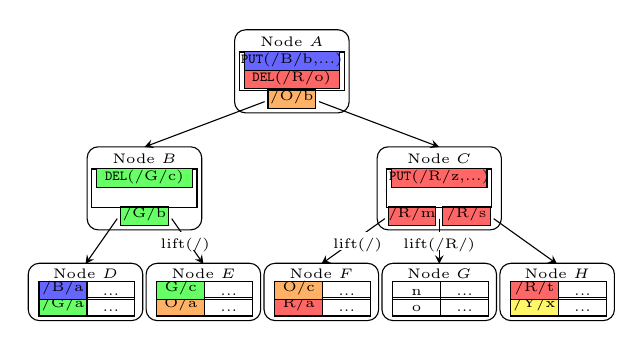
\begin{tikzpicture}[xscale=0.95, yscale=0.95]
            \node[anchor=south, rectangle, rounded corners, minimum height=.06\textwidth, minimum width=.12\textwidth, draw=black] at (0, 0) {};
            \node[anchor=south, font=\tiny] at (0, .036\textwidth) {Node $F$};
            \node[anchor=south, rectangle, minimum height=.015\textwidth, minimum width=.05\textwidth, draw=black, fill={red!60}] at (-.025\textwidth, .005\textwidth) {};
            \node[anchor=south, font=\tiny] at (-.025\textwidth, 0) {R/a};
            \node[anchor=south, rectangle, minimum height=.015\textwidth, minimum width=.05\textwidth, draw=black] at (.028\textwidth, .005\textwidth) {};
            \node[anchor=south, font=\tiny] at (.028\textwidth, 0) {...};
            \node[anchor=south, rectangle, minimum height=.015\textwidth, minimum width=.05\textwidth, draw=black, fill={orange!60}] at (-.025\textwidth, .023\textwidth) {};
            \node[anchor=south, font=\tiny] at (-.025\textwidth, .018\textwidth) {O/c};
            \node[anchor=south, rectangle, minimum height=.015\textwidth, minimum width=.05\textwidth, draw=black] at (.028\textwidth, .023\textwidth) {};
            \node[anchor=south, font=\tiny] at (.028\textwidth, .018\textwidth) {...};

            \node[anchor=south, rectangle, rounded corners, minimum height=.06\textwidth, minimum width=.12\textwidth, draw=black] at (.13\textwidth, 0) {};
            \node[anchor=south, font=\tiny] at (.13\textwidth, .036\textwidth) {Node $G$};
            \node[anchor=south, rectangle, minimum height=.015\textwidth, minimum width=.05\textwidth, draw=black] at (.105\textwidth, .005\textwidth) {};
            \node[anchor=south, font=\tiny] at (.105\textwidth, 0) {o};
            \node[anchor=south, rectangle, minimum height=.015\textwidth, minimum width=.05\textwidth, draw=black] at (.158\textwidth, .005\textwidth) {};
            \node[anchor=south, font=\tiny] at (.158\textwidth, 0) {...};
            \node[anchor=south, rectangle, minimum height=.015\textwidth, minimum width=.05\textwidth, draw=black] at (.105\textwidth, .023\textwidth) {};
            \node[anchor=south, font=\tiny] at (.105\textwidth, .018\textwidth) {n};
            \node[anchor=south, rectangle, minimum height=.015\textwidth, minimum width=.05\textwidth, draw=black] at (.158\textwidth, .023\textwidth) {};
            \node[anchor=south, font=\tiny] at (.158\textwidth, .018\textwidth) {...};

            \node[anchor=south, rectangle, rounded corners, minimum height=.06\textwidth, minimum width=.12\textwidth, draw=black] at (.26\textwidth, 0) {};
            \node[anchor=south, font=\tiny] at (.26\textwidth, .036\textwidth) {Node $H$};
            \node[anchor=south, rectangle, minimum height=.015\textwidth, minimum width=.05\textwidth, draw=black, fill={yellow!60}] at (.235\textwidth, .005\textwidth) {};
            \node[anchor=south, font=\tiny] at (.235\textwidth, 0) {/Y/x};
            \node[anchor=south, rectangle, minimum height=.015\textwidth, minimum width=.05\textwidth, draw=black] at (.288\textwidth, .005\textwidth) {};
            \node[anchor=south, font=\tiny] at (.288\textwidth, 0) {...};
            \node[anchor=south, rectangle, minimum height=.015\textwidth, minimum width=.05\textwidth, draw=black, fill={red!60}] at (.235\textwidth, .023\textwidth) {};
            \node[anchor=south, font=\tiny] at (.235\textwidth, .018\textwidth) {/R/t};
            \node[anchor=south, rectangle, minimum height=.015\textwidth, minimum width=.05\textwidth, draw=black] at (.288\textwidth, .023\textwidth) {};
            \node[anchor=south, font=\tiny] at (.288\textwidth, .018\textwidth) {...};

            \node[anchor=south, rectangle, rounded corners, minimum height=.06\textwidth, minimum width=.12\textwidth, draw=black] at (-.13\textwidth, 0) {};
            \node[anchor=south, font=\tiny] at (-.13\textwidth, .036\textwidth) {Node $E$};
            \node[anchor=south, rectangle, minimum height=.015\textwidth, minimum width=.05\textwidth, draw=black, fill={orange!60}] at (-.155\textwidth, .005\textwidth) {};
            \node[anchor=south, font=\tiny] at (-.155\textwidth, 0) {O/a};
            \node[anchor=south, rectangle, minimum height=.015\textwidth, minimum width=.05\textwidth, draw=black] at (-.102\textwidth, .005\textwidth) {};
            \node[anchor=south, font=\tiny] at (-.102\textwidth, 0) {...};
            \node[anchor=south, rectangle, minimum height=.015\textwidth, minimum width=.05\textwidth, draw=black, fill={green!60}] at (-.155\textwidth, .023\textwidth) {};
            \node[anchor=south, font=\tiny] at (-.155\textwidth, .018\textwidth) {G/c};
            \node[anchor=south, rectangle, minimum height=.015\textwidth, minimum width=.05\textwidth, draw=black] at (-.102\textwidth, .023\textwidth) {};
            \node[anchor=south, font=\tiny] at (-.102\textwidth, .018\textwidth) {...};

            \node[anchor=south, rectangle, rounded corners, minimum height=.06\textwidth, minimum width=.12\textwidth, draw=black] at (-.26\textwidth, 0) {};
            \node[anchor=south, font=\tiny] at (-.26\textwidth, .036\textwidth) {Node $D$};
            \node[anchor=south, rectangle, minimum height=.015\textwidth, minimum width=.05\textwidth, draw=black, fill={green!60}] at (-.285\textwidth, .005\textwidth) {};
            \node[anchor=south, font=\tiny] at (-.285\textwidth, 0) {/G/a};
            \node[anchor=south, rectangle, minimum height=.015\textwidth, minimum width=.05\textwidth, draw=black] at (-.232\textwidth, .005\textwidth) {};
            \node[anchor=south, font=\tiny] at (-.232\textwidth, 0) {...};
            \node[anchor=south, rectangle, minimum height=.015\textwidth, minimum width=.05\textwidth, draw=black, fill={blue!60}] at (-.285\textwidth, .023\textwidth) {};
            \node[anchor=south, font=\tiny] at (-.285\textwidth, .018\textwidth) {/B/a};
            \node[anchor=south, rectangle, minimum height=.015\textwidth, minimum width=.05\textwidth, draw=black] at (-.232\textwidth, .023\textwidth) {};
            \node[anchor=south, font=\tiny] at (-.232\textwidth, .018\textwidth) {...};

            \node[anchor=south, rectangle, rounded corners, minimum height=.087\textwidth, minimum width=.12\textwidth, draw=black] at (-.195\textwidth, .1\textwidth) {};
            \node[anchor=south, font=\tiny] at (-.195\textwidth, .163\textwidth) {Node $B$};
            \node[anchor=south, rectangle, minimum height=.015\textwidth, minimum width=.05\textwidth, draw=black, fill={green!60}] at (-.195\textwidth, .105\textwidth) {};
            \node[anchor=south, font=\tiny] at (-.195\textwidth, .1\textwidth) {/G/b};
            \node[anchor=south, rectangle, minimum height=.04\textwidth, minimum width=.11\textwidth, draw=black] at (-.195\textwidth, .125\textwidth) {};
            \node[anchor=south, rectangle, minimum height=.015\textwidth, minimum width=.1\textwidth, draw=black, fill={green!60}] at (-.195\textwidth, .147\textwidth) {};
            \node[anchor=south, font=\tiny] at  (-.195\textwidth, .141\textwidth) {\delm(/G/c)};

            \node[anchor=south, rectangle, rounded corners, minimum height=.087\textwidth, minimum width=.13\textwidth, draw=black] at (.13\textwidth, .1\textwidth) {};
            \node[anchor=south, font=\tiny] at (.13\textwidth, .163\textwidth) {Node $C$};
            \node[anchor=south, rectangle, minimum height=.015\textwidth, minimum width=.05\textwidth, draw=black, fill={red!60}] at (.1\textwidth, .105\textwidth) {};
            \node[anchor=south, font=\tiny] at (.1\textwidth, .1\textwidth) {/R/m};
            \node[anchor=south, rectangle, minimum height=.015\textwidth, minimum width=.05\textwidth, draw=black, fill={red!60}] at (.16\textwidth, .105\textwidth) {};
            \node[anchor=south, font=\tiny] at (.16\textwidth, .1\textwidth) {/R/s};
            \node[anchor=south, rectangle, minimum height=.04\textwidth, minimum width=.11\textwidth, draw=black] at (.13\textwidth, .125\textwidth) {};
            \node[anchor=south, rectangle, minimum height=.015\textwidth, minimum width=.1\textwidth, draw=black, fill={red!60}] at (.13\textwidth, .147\textwidth) {};
            \node[anchor=south, font=\tiny] at  (.13\textwidth, .141\textwidth) {\putm(/R/z,...)};

            \node[anchor=south, rectangle, rounded corners, minimum height=.087\textwidth, minimum width=.12\textwidth, draw=black] at (-.0325\textwidth, .229\textwidth) {};
            \node[anchor=south, font=\tiny] at (-.0325\textwidth, .292\textwidth) {Node $A$};
            \node[anchor=south, rectangle, minimum height=.015\textwidth, minimum width=.05\textwidth, draw=black, fill={orange!60}] at (-.0325\textwidth, .234\textwidth) {};
            \node[anchor=south, font=\tiny] at (-.0325\textwidth, .229\textwidth) {/O/b};
            \node[anchor=south, rectangle, minimum height=.04\textwidth, minimum width=.11\textwidth, draw=black] at (-.0325\textwidth, .254\textwidth) {};
            \node[anchor=south, rectangle, minimum height=.015\textwidth, minimum width=.1\textwidth, draw=black, fill={red!60}] at (-.0325\textwidth, .256\textwidth) {};
            \node[anchor=south, font=\tiny] at  (-.0325\textwidth, .25\textwidth) {\delm(/R/o)};
            \node[anchor=south, rectangle, minimum height=.015\textwidth, minimum width=.1\textwidth, draw=black, fill={blue!60}] at (-.0325\textwidth, .276\textwidth) {};
            \node[anchor=south, font=\tiny] at  (-.0325\textwidth, .27\textwidth) {\putm(/B/b,...)};

            \draw[->, >=stealth] (-.225\textwidth, .113\textwidth) -- (-.26\textwidth, .063\textwidth);
            \draw[->, >=stealth] (-.165\textwidth, .113\textwidth) -- (-.13\textwidth, .063\textwidth);
            \draw[->, >=stealth] (.13\textwidth, .113\textwidth) -- (.13\textwidth, .063\textwidth);
            \draw[->, >=stealth] (.19\textwidth, .113\textwidth) -- (.26\textwidth, .063\textwidth);
            \draw[->, >=stealth] (.07\textwidth, .113\textwidth) -- (0, .063\textwidth);
            \draw[->, >=stealth] (-.0625\textwidth, .242\textwidth) -- (-.195\textwidth, .192\textwidth);
            \draw[->, >=stealth] (-.0025\textwidth, .242\textwidth) -- (.13\textwidth, .192\textwidth);

            \node[anchor=north,rectangle, minimum height=.015\textwidth, minimum width=.05\textwidth, fill={white}] at (.13\textwidth, .099\textwidth) {};
            \node[anchor=north, font=\tiny] at (.13\textwidth, .102\textwidth) {lift(/R/)};
            \node[anchor=north,rectangle, minimum height=.015\textwidth, minimum width=.05\textwidth, fill={white}] at (.04\textwidth, .099\textwidth) {};
            \node[anchor=north, font=\tiny] at (.04\textwidth, .102\textwidth) {lift(/)};
            \node[anchor=north,rectangle, minimum height=.015\textwidth, minimum width=.05\textwidth, fill={white}] at (-.15\textwidth, .099\textwidth) {};
            \node[anchor=north, font=\tiny] at (-.15\textwidth, .102\textwidth) {lift(/)};
        \end{tikzpicture}
        \caption{\label{subfig:goto-1} The \bet before the range-clone.}
    \end{subfigure}
    \begin{subfigure}{\textwidth}
        \centering
        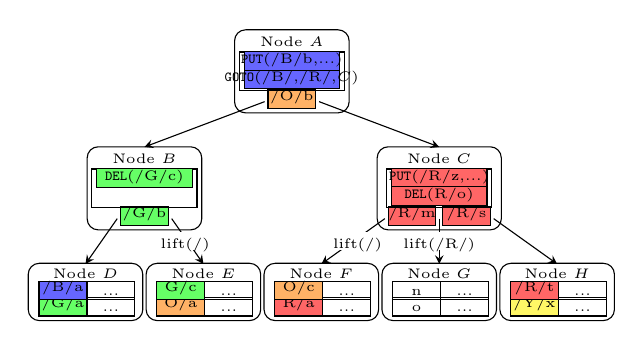
\begin{tikzpicture}[xscale=0.95, yscale=0.95]
            \node[anchor=south, rectangle, rounded corners, minimum height=.06\textwidth, minimum width=.12\textwidth, draw=black] at (0, 0) {};
            \node[anchor=south, font=\tiny] at (0, .036\textwidth) {Node $F$};
            \node[anchor=south, rectangle, minimum height=.015\textwidth, minimum width=.05\textwidth, draw=black, fill={red!60}] at (-.025\textwidth, .005\textwidth) {};
            \node[anchor=south, font=\tiny] at (-.025\textwidth, 0) {R/a};
            \node[anchor=south, rectangle, minimum height=.015\textwidth, minimum width=.05\textwidth, draw=black] at (.028\textwidth, .005\textwidth) {};
            \node[anchor=south, font=\tiny] at (.028\textwidth, 0) {...};
            \node[anchor=south, rectangle, minimum height=.015\textwidth, minimum width=.05\textwidth, draw=black, fill={orange!60}] at (-.025\textwidth, .023\textwidth) {};
            \node[anchor=south, font=\tiny] at (-.025\textwidth, .018\textwidth) {O/c};
            \node[anchor=south, rectangle, minimum height=.015\textwidth, minimum width=.05\textwidth, draw=black] at (.028\textwidth, .023\textwidth) {};
            \node[anchor=south, font=\tiny] at (.028\textwidth, .018\textwidth) {...};

            \node[anchor=south, rectangle, rounded corners, minimum height=.06\textwidth, minimum width=.12\textwidth, draw=black] at (.13\textwidth, 0) {};
            \node[anchor=south, font=\tiny] at (.13\textwidth, .036\textwidth) {Node $G$};
            \node[anchor=south, rectangle, minimum height=.015\textwidth, minimum width=.05\textwidth, draw=black] at (.105\textwidth, .005\textwidth) {};
            \node[anchor=south, font=\tiny] at (.105\textwidth, 0) {o};
            \node[anchor=south, rectangle, minimum height=.015\textwidth, minimum width=.05\textwidth, draw=black] at (.158\textwidth, .005\textwidth) {};
            \node[anchor=south, font=\tiny] at (.158\textwidth, 0) {...};
            \node[anchor=south, rectangle, minimum height=.015\textwidth, minimum width=.05\textwidth, draw=black] at (.105\textwidth, .023\textwidth) {};
            \node[anchor=south, font=\tiny] at (.105\textwidth, .018\textwidth) {n};
            \node[anchor=south, rectangle, minimum height=.015\textwidth, minimum width=.05\textwidth, draw=black] at (.158\textwidth, .023\textwidth) {};
            \node[anchor=south, font=\tiny] at (.158\textwidth, .018\textwidth) {...};

            \node[anchor=south, rectangle, rounded corners, minimum height=.06\textwidth, minimum width=.12\textwidth, draw=black] at (.26\textwidth, 0) {};
            \node[anchor=south, font=\tiny] at (.26\textwidth, .036\textwidth) {Node $H$};
            \node[anchor=south, rectangle, minimum height=.015\textwidth, minimum width=.05\textwidth, draw=black, fill={yellow!60}] at (.235\textwidth, .005\textwidth) {};
            \node[anchor=south, font=\tiny] at (.235\textwidth, 0) {/Y/x};
            \node[anchor=south, rectangle, minimum height=.015\textwidth, minimum width=.05\textwidth, draw=black] at (.288\textwidth, .005\textwidth) {};
            \node[anchor=south, font=\tiny] at (.288\textwidth, 0) {...};
            \node[anchor=south, rectangle, minimum height=.015\textwidth, minimum width=.05\textwidth, draw=black, fill={red!60}] at (.235\textwidth, .023\textwidth) {};
            \node[anchor=south, font=\tiny] at (.235\textwidth, .018\textwidth) {/R/t};
            \node[anchor=south, rectangle, minimum height=.015\textwidth, minimum width=.05\textwidth, draw=black] at (.288\textwidth, .023\textwidth) {};
            \node[anchor=south, font=\tiny] at (.288\textwidth, .018\textwidth) {...};

            \node[anchor=south, rectangle, rounded corners, minimum height=.06\textwidth, minimum width=.12\textwidth, draw=black] at (-.13\textwidth, 0) {};
            \node[anchor=south, font=\tiny] at (-.13\textwidth, .036\textwidth) {Node $E$};
            \node[anchor=south, rectangle, minimum height=.015\textwidth, minimum width=.05\textwidth, draw=black, fill={orange!60}] at (-.155\textwidth, .005\textwidth) {};
            \node[anchor=south, font=\tiny] at (-.155\textwidth, 0) {O/a};
            \node[anchor=south, rectangle, minimum height=.015\textwidth, minimum width=.05\textwidth, draw=black] at (-.102\textwidth, .005\textwidth) {};
            \node[anchor=south, font=\tiny] at (-.102\textwidth, 0) {...};
            \node[anchor=south, rectangle, minimum height=.015\textwidth, minimum width=.05\textwidth, draw=black, fill={green!60}] at (-.155\textwidth, .023\textwidth) {};
            \node[anchor=south, font=\tiny] at (-.155\textwidth, .018\textwidth) {G/c};
            \node[anchor=south, rectangle, minimum height=.015\textwidth, minimum width=.05\textwidth, draw=black] at (-.102\textwidth, .023\textwidth) {};
            \node[anchor=south, font=\tiny] at (-.102\textwidth, .018\textwidth) {...};

            \node[anchor=south, rectangle, rounded corners, minimum height=.06\textwidth, minimum width=.12\textwidth, draw=black] at (-.26\textwidth, 0) {};
            \node[anchor=south, font=\tiny] at (-.26\textwidth, .036\textwidth) {Node $D$};
            \node[anchor=south, rectangle, minimum height=.015\textwidth, minimum width=.05\textwidth, draw=black, fill={green!60}] at (-.285\textwidth, .005\textwidth) {};
            \node[anchor=south, font=\tiny] at (-.285\textwidth, 0) {/G/a};
            \node[anchor=south, rectangle, minimum height=.015\textwidth, minimum width=.05\textwidth, draw=black] at (-.232\textwidth, .005\textwidth) {};
            \node[anchor=south, font=\tiny] at (-.232\textwidth, 0) {...};
            \node[anchor=south, rectangle, minimum height=.015\textwidth, minimum width=.05\textwidth, draw=black, fill={blue!60}] at (-.285\textwidth, .023\textwidth) {};
            \node[anchor=south, font=\tiny] at (-.285\textwidth, .018\textwidth) {/B/a};
            \node[anchor=south, rectangle, minimum height=.015\textwidth, minimum width=.05\textwidth, draw=black] at (-.232\textwidth, .023\textwidth) {};
            \node[anchor=south, font=\tiny] at (-.232\textwidth, .018\textwidth) {...};

            \node[anchor=south, rectangle, rounded corners, minimum height=.087\textwidth, minimum width=.12\textwidth, draw=black] at (-.195\textwidth, .1\textwidth) {};
            \node[anchor=south, font=\tiny] at (-.195\textwidth, .163\textwidth) {Node $B$};
            \node[anchor=south, rectangle, minimum height=.015\textwidth, minimum width=.05\textwidth, draw=black, fill={green!60}] at (-.195\textwidth, .105\textwidth) {};
            \node[anchor=south, font=\tiny] at (-.195\textwidth, .1\textwidth) {/G/b};
            \node[anchor=south, rectangle, minimum height=.04\textwidth, minimum width=.11\textwidth, draw=black] at (-.195\textwidth, .125\textwidth) {};
            \node[anchor=south, rectangle, minimum height=.015\textwidth, minimum width=.1\textwidth, draw=black, fill={green!60}] at (-.195\textwidth, .147\textwidth) {};
            \node[anchor=south, font=\tiny] at  (-.195\textwidth, .141\textwidth) {\delm(/G/c)};

            \node[anchor=south, rectangle, rounded corners, minimum height=.087\textwidth, minimum width=.13\textwidth, draw=black] at (.13\textwidth, .1\textwidth) {};
            \node[anchor=south, font=\tiny] at (.13\textwidth, .163\textwidth) {Node $C$};
            \node[anchor=south, rectangle, minimum height=.015\textwidth, minimum width=.05\textwidth, draw=black, fill={red!60}] at (.1\textwidth, .105\textwidth) {};
            \node[anchor=south, font=\tiny] at (.1\textwidth, .1\textwidth) {/R/m};
            \node[anchor=south, rectangle, minimum height=.015\textwidth, minimum width=.05\textwidth, draw=black, fill={red!60}] at (.16\textwidth, .105\textwidth) {};
            \node[anchor=south, font=\tiny] at (.16\textwidth, .1\textwidth) {/R/s};
            \node[anchor=south, rectangle, minimum height=.04\textwidth, minimum width=.11\textwidth, draw=black] at (.13\textwidth, .125\textwidth) {};
            \node[anchor=south, rectangle, minimum height=.015\textwidth, minimum width=.1\textwidth, draw=black, fill={red!60}] at (.13\textwidth, .147\textwidth) {};
            \node[anchor=south, font=\tiny] at  (.13\textwidth, .141\textwidth) {\putm(/R/z,...)};
            \node[anchor=south, rectangle, minimum height=.015\textwidth, minimum width=.1\textwidth, draw=black, fill={red!60}] at (.13\textwidth, .127\textwidth) {};
            \node[anchor=south, font=\tiny] at  (.13\textwidth, .121\textwidth) {\delm(R/o)};

            \node[anchor=south, rectangle, rounded corners, minimum height=.087\textwidth, minimum width=.12\textwidth, draw=black] at (-.0325\textwidth, .229\textwidth) {};
            \node[anchor=south, font=\tiny] at (-.0325\textwidth, .292\textwidth) {Node $A$};
            \node[anchor=south, rectangle, minimum height=.015\textwidth, minimum width=.05\textwidth, draw=black, fill={orange!60}] at (-.0325\textwidth, .234\textwidth) {};
            \node[anchor=south, font=\tiny] at (-.0325\textwidth, .229\textwidth) {/O/b};
            \node[anchor=south, rectangle, minimum height=.04\textwidth, minimum width=.11\textwidth, draw=black] at (-.0325\textwidth, .254\textwidth) {};
            \node[anchor=south, rectangle, minimum height=.015\textwidth, minimum width=.1\textwidth, draw=black, fill={blue!60}] at (-.0325\textwidth, .256\textwidth) {};
            \node[anchor=south, font=\tiny] at  (-.0325\textwidth, .25\textwidth) {\goto(/B/,/R/,$C$)};
            \node[anchor=south, rectangle, minimum height=.015\textwidth, minimum width=.1\textwidth, draw=black, fill={blue!60}] at (-.0325\textwidth, .276\textwidth) {};
            \node[anchor=south, font=\tiny] at  (-.0325\textwidth, .27\textwidth) {\putm(/B/b,...)};

            \draw[->, >=stealth] (-.225\textwidth, .113\textwidth) -- (-.26\textwidth, .063\textwidth);
            \draw[->, >=stealth] (-.165\textwidth, .113\textwidth) -- (-.13\textwidth, .063\textwidth);
            \draw[->, >=stealth] (.13\textwidth, .113\textwidth) -- (.13\textwidth, .063\textwidth);
            \draw[->, >=stealth] (.19\textwidth, .113\textwidth) -- (.26\textwidth, .063\textwidth);
            \draw[->, >=stealth] (.07\textwidth, .113\textwidth) -- (0, .063\textwidth);
            \draw[->, >=stealth] (-.0625\textwidth, .242\textwidth) -- (-.195\textwidth, .192\textwidth);
            \draw[->, >=stealth] (-.0025\textwidth, .242\textwidth) -- (.13\textwidth, .192\textwidth);

            \node[anchor=north,rectangle, minimum height=.015\textwidth, minimum width=.05\textwidth, fill={white}] at (.13\textwidth, .099\textwidth) {};
            \node[anchor=north, font=\tiny] at (.13\textwidth, .102\textwidth) {lift(/R/)};
            \node[anchor=north,rectangle, minimum height=.015\textwidth, minimum width=.05\textwidth, fill={white}] at (.04\textwidth, .099\textwidth) {};
            \node[anchor=north, font=\tiny] at (.04\textwidth, .102\textwidth) {lift(/)};
            \node[anchor=north,rectangle, minimum height=.015\textwidth, minimum width=.05\textwidth, fill={white}] at (-.15\textwidth, .099\textwidth) {};
            \node[anchor=north, font=\tiny] at (-.15\textwidth, .102\textwidth) {lift(/)};
        \end{tikzpicture}
        \caption{\label{subfig:goto-2} The range-clone operation generates a \goto message
            for destination (``/B/'') keys.}
    \end{subfigure}
    \caption[A range-clone example with a \goto message]{\label{fig:goto}
        An example of completing range-clone(``/R/'', ``/B/'') with a \goto message.}
\end{figure}

\paragraph{Range-clone with \goto messages.}

Range-clone(\spre, \dpre) can be implement with \goto messages through the
following steps:
\begin{itemize}
\item it performs a root-to-leaf traversal with \spre until reaching the source
LCA, flushing messages from parent to child simultaneously.
At this point, all messages with source keys are in the subtree rooted at the
source LCA.
\item it then injects a \goto message into the root node of the lifted \bedag
with the source LCA as the node ID in the \goto message, increasing the
reference count of the source LCA by 1.
Note, the \spre in the \goto message can be different from the \spre of the
range-clone operation,
because the root-to-leaf traversal may lift some prefix from the \spre.
\end{itemize}
Note, this range-clone operation doesn't perform any node split on the critical
path.

Figure~\ref{fig:goto} shows an example of range-clone(``/R/'', ``/B/'')
that generates a \goto message.
Starting from the root node, Node $A$, the range-clone operation traverses to
the source LCA, Node $C$.
At the same time, it flushes the message, \delm(``/R/z''), to Node $C$.
Then, the range-clone range then injects a \goto message into the root node,
with ``/B/'' as its \dpre, ``/R/'' as its \spre and Node $C$ as its node ID.
Figure~\ref{subfig:goto-2} shows the result.
Now, consider a query for key ``/B/a''.
The query starts at the Node $A$.
Then, instead of following the parent-to-child pointers to Node $B$, it follows
the \goto message and visit Node $C$.
The \goto message also acts as a \xf function that translates the search key
to ``/R/a'' and bounds the result in range (``/R/a$_{min}$'', ``/R/$_{max}$'').
At last, the query finds the correct key/value pair in Node $F$.

\subsection{Flushing \goto messages.}

The lifted \bedag should flush \goto messages alongside with other messages.
Otherwise, the root node can be filled with \goto messages.
In the simple case, the node that tries to flush a \goto message has a single
child that covers the key range of the \goto message
and the child is higher than the source LCA of the \goto message.
Flushing the \goto message simply lifts the \dpre of the \goto message and moves
the \goto message from the parent buffer to the child buffer.

\paragraph{The \bedag merges children before flushing a \goto message.}

\begin{figure}
    \begin{subfigure}{\textwidth}
        \centering
        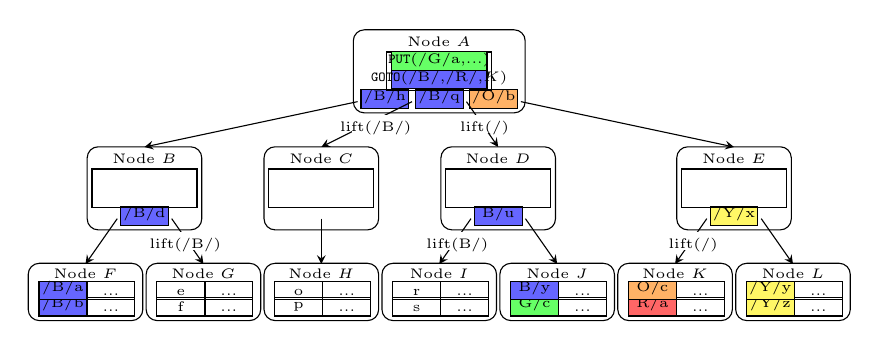
\begin{tikzpicture}[xscale=0.95, yscale=0.95]
            \node[anchor=south, rectangle, rounded corners, minimum height=.06\textwidth, minimum width=.12\textwidth, draw=black] at (0, 0) {};
            \node[anchor=south, font=\tiny] at (0, .036\textwidth) {Node $F$};
            \node[anchor=south, rectangle, minimum height=.015\textwidth, minimum width=.05\textwidth, draw=black, fill={blue!60}] at (-.025\textwidth, .005\textwidth) {};
            \node[anchor=south, font=\tiny] at (-.025\textwidth, 0) {/B/b};
            \node[anchor=south, rectangle, minimum height=.015\textwidth, minimum width=.05\textwidth, draw=black] at (.028\textwidth, .005\textwidth) {};
            \node[anchor=south, font=\tiny] at (.028\textwidth, 0) {...};
            \node[anchor=south, rectangle, minimum height=.015\textwidth, minimum width=.05\textwidth, draw=black, fill={blue!60}] at (-.025\textwidth, .023\textwidth) {};
            \node[anchor=south, font=\tiny] at (-.025\textwidth, .018\textwidth) {/B/a};
            \node[anchor=south, rectangle, minimum height=.015\textwidth, minimum width=.05\textwidth, draw=black] at (.028\textwidth, .023\textwidth) {};
            \node[anchor=south, font=\tiny] at (.028\textwidth, .018\textwidth) {...};

            \node[anchor=south, rectangle, rounded corners, minimum height=.06\textwidth, minimum width=.12\textwidth, draw=black] at (.13\textwidth, 0) {};
            \node[anchor=south, font=\tiny] at (.13\textwidth, .036\textwidth) {Node $G$};
            \node[anchor=south, rectangle, minimum height=.015\textwidth, minimum width=.05\textwidth, draw=black] at (.105\textwidth, .005\textwidth) {};
            \node[anchor=south, font=\tiny] at (.105\textwidth, 0) {f};
            \node[anchor=south, rectangle, minimum height=.015\textwidth, minimum width=.05\textwidth, draw=black] at (.158\textwidth, .005\textwidth) {};
            \node[anchor=south, font=\tiny] at (.158\textwidth, 0) {...};
            \node[anchor=south, rectangle, minimum height=.015\textwidth, minimum width=.05\textwidth, draw=black] at (.105\textwidth, .023\textwidth) {};
            \node[anchor=south, font=\tiny] at (.105\textwidth, .018\textwidth) {e};
            \node[anchor=south, rectangle, minimum height=.015\textwidth, minimum width=.05\textwidth, draw=black] at (.158\textwidth, .023\textwidth) {};
            \node[anchor=south, font=\tiny] at (.158\textwidth, .018\textwidth) {...};

            \node[anchor=south, rectangle, rounded corners, minimum height=.06\textwidth, minimum width=.12\textwidth, draw=black] at (.26\textwidth, 0) {};
            \node[anchor=south, font=\tiny] at (.26\textwidth, .036\textwidth) {Node $H$};
            \node[anchor=south, rectangle, minimum height=.015\textwidth, minimum width=.05\textwidth, draw=black] at (.235\textwidth, .005\textwidth) {};
            \node[anchor=south, font=\tiny] at (.235\textwidth, 0) {p};
            \node[anchor=south, rectangle, minimum height=.015\textwidth, minimum width=.05\textwidth, draw=black] at (.288\textwidth, .005\textwidth) {};
            \node[anchor=south, font=\tiny] at (.288\textwidth, 0) {...};
            \node[anchor=south, rectangle, minimum height=.015\textwidth, minimum width=.05\textwidth, draw=black] at (.235\textwidth, .023\textwidth) {};
            \node[anchor=south, font=\tiny] at (.235\textwidth, .018\textwidth) {o};
            \node[anchor=south, rectangle, minimum height=.015\textwidth, minimum width=.05\textwidth, draw=black] at (.288\textwidth, .023\textwidth) {};
            \node[anchor=south, font=\tiny] at (.288\textwidth, .018\textwidth) {...};

            \node[anchor=south, rectangle, rounded corners, minimum height=.06\textwidth, minimum width=.12\textwidth, draw=black] at (.39\textwidth, 0) {};
            \node[anchor=south, font=\tiny] at (.39\textwidth, .036\textwidth) {Node $I$};
            \node[anchor=south, rectangle, minimum height=.015\textwidth, minimum width=.05\textwidth, draw=black] at (.365\textwidth, .005\textwidth) {};
            \node[anchor=south, font=\tiny] at (.365\textwidth, 0) {s};
            \node[anchor=south, rectangle, minimum height=.015\textwidth, minimum width=.05\textwidth, draw=black] at (.418\textwidth, .005\textwidth) {};
            \node[anchor=south, font=\tiny] at (.418\textwidth, 0) {...};
            \node[anchor=south, rectangle, minimum height=.015\textwidth, minimum width=.05\textwidth, draw=black] at (.365\textwidth, .023\textwidth) {};
            \node[anchor=south, font=\tiny] at (.365\textwidth, .018\textwidth) {r};
            \node[anchor=south, rectangle, minimum height=.015\textwidth, minimum width=.05\textwidth, draw=black] at (.418\textwidth, .023\textwidth) {};
            \node[anchor=south, font=\tiny] at (.418\textwidth, .018\textwidth) {...};

            \node[anchor=south, rectangle, rounded corners, minimum height=.06\textwidth, minimum width=.12\textwidth, draw=black] at (.52\textwidth, 0) {};
            \node[anchor=south, font=\tiny] at (.52\textwidth, .036\textwidth) {Node $J$};
            \node[anchor=south, rectangle, minimum height=.015\textwidth, minimum width=.05\textwidth, draw=black, fill={green!60}] at (.495\textwidth, .005\textwidth) {};
            \node[anchor=south, font=\tiny] at (.495\textwidth, 0) {G/c};
            \node[anchor=south, rectangle, minimum height=.015\textwidth, minimum width=.05\textwidth, draw=black] at (.548\textwidth, .005\textwidth) {};
            \node[anchor=south, font=\tiny] at (.548\textwidth, 0) {...};
            \node[anchor=south, rectangle, minimum height=.015\textwidth, minimum width=.05\textwidth, draw=black, fill={blue!60}] at (.495\textwidth, .023\textwidth) {};
            \node[anchor=south, font=\tiny] at (.495\textwidth, .018\textwidth) {B/y};
            \node[anchor=south, rectangle, minimum height=.015\textwidth, minimum width=.05\textwidth, draw=black] at (.548\textwidth, .023\textwidth) {};
            \node[anchor=south, font=\tiny] at (.548\textwidth, .018\textwidth) {...};

            \node[anchor=south, rectangle, rounded corners, minimum height=.06\textwidth, minimum width=.12\textwidth, draw=black] at (.65\textwidth, 0) {};
            \node[anchor=south, font=\tiny] at (.65\textwidth, .036\textwidth) {Node $K$};
            \node[anchor=south, rectangle, minimum height=.015\textwidth, minimum width=.05\textwidth, draw=black, fill={red!60}] at (.625\textwidth, .005\textwidth) {};
            \node[anchor=south, font=\tiny] at (.625\textwidth, 0) {R/a};
            \node[anchor=south, rectangle, minimum height=.015\textwidth, minimum width=.05\textwidth, draw=black] at (.678\textwidth, .005\textwidth) {};
            \node[anchor=south, font=\tiny] at (.678\textwidth, 0) {...};
            \node[anchor=south, rectangle, minimum height=.015\textwidth, minimum width=.05\textwidth, draw=black, fill={orange!60}] at (.625\textwidth, .023\textwidth) {};
            \node[anchor=south, font=\tiny] at (.625\textwidth, .018\textwidth) {O/c};
            \node[anchor=south, rectangle, minimum height=.015\textwidth, minimum width=.05\textwidth, draw=black] at (.678\textwidth, .023\textwidth) {};
            \node[anchor=south, font=\tiny] at (.678\textwidth, .018\textwidth) {...};

            \node[anchor=south, rectangle, rounded corners, minimum height=.06\textwidth, minimum width=.12\textwidth, draw=black] at (.78\textwidth, 0) {};
            \node[anchor=south, font=\tiny] at (.78\textwidth, .036\textwidth) {Node $L$};
            \node[anchor=south, rectangle, minimum height=.015\textwidth, minimum width=.05\textwidth, draw=black, fill={yellow!60}] at (.755\textwidth, .005\textwidth) {};
            \node[anchor=south, font=\tiny] at (.755\textwidth, 0) {/Y/z};
            \node[anchor=south, rectangle, minimum height=.015\textwidth, minimum width=.05\textwidth, draw=black] at (.808\textwidth, .005\textwidth) {};
            \node[anchor=south, font=\tiny] at (.808\textwidth, 0) {...};
            \node[anchor=south, rectangle, minimum height=.015\textwidth, minimum width=.05\textwidth, draw=black, fill={yellow!60}] at (.755\textwidth, .023\textwidth) {};
            \node[anchor=south, font=\tiny] at (.755\textwidth, .018\textwidth) {/Y/y};
            \node[anchor=south, rectangle, minimum height=.015\textwidth, minimum width=.05\textwidth, draw=black] at (.808\textwidth, .023\textwidth) {};
            \node[anchor=south, font=\tiny] at (.808\textwidth, .018\textwidth) {...};

            \node[anchor=south, rectangle, rounded corners, minimum height=.087\textwidth, minimum width=.12\textwidth, draw=black] at (.065\textwidth, .1\textwidth) {};
            \node[anchor=south, font=\tiny] at (.065\textwidth, .163\textwidth) {Node $B$};
            \node[anchor=south, rectangle, minimum height=.015\textwidth, minimum width=.05\textwidth, draw=black, fill={blue!60}] at (.065\textwidth, .105\textwidth) {};
            \node[anchor=south, font=\tiny] at (.065\textwidth, .1\textwidth) {/B/d};
            \node[anchor=south, rectangle, minimum height=.04\textwidth, minimum width=.11\textwidth, draw=black] at (.065\textwidth, .125\textwidth) {};

            \node[anchor=south, rectangle, rounded corners, minimum height=.087\textwidth, minimum width=.12\textwidth, draw=black] at (.26\textwidth, .1\textwidth) {};
            \node[anchor=south, font=\tiny] at (.26\textwidth, .163\textwidth) {Node $C$};
            \node[anchor=south, rectangle, minimum height=.04\textwidth, minimum width=.11\textwidth, draw=black] at (.26\textwidth, .125\textwidth) {};

            \node[anchor=south, rectangle, rounded corners, minimum height=.087\textwidth, minimum width=.12\textwidth, draw=black] at (.455\textwidth, .1\textwidth) {};
            \node[anchor=south, font=\tiny] at (.455\textwidth, .163\textwidth) {Node $D$};
            \node[anchor=south, rectangle, minimum height=.015\textwidth, minimum width=.05\textwidth, draw=black, fill={blue!60}] at (.455\textwidth, .105\textwidth) {};
            \node[anchor=south, font=\tiny] at (.455\textwidth, .1\textwidth) {B/u};
            \node[anchor=south, rectangle, minimum height=.04\textwidth, minimum width=.11\textwidth, draw=black] at (.455\textwidth, .125\textwidth) {};

            \node[anchor=south, rectangle, rounded corners, minimum height=.087\textwidth, minimum width=.12\textwidth, draw=black] at (.715\textwidth, .1\textwidth) {};
            \node[anchor=south, font=\tiny] at (.715\textwidth, .163\textwidth) {Node $E$};
            \node[anchor=south, rectangle, minimum height=.015\textwidth, minimum width=.05\textwidth, draw=black, fill={yellow!60}] at (.715\textwidth, .105\textwidth) {};
            \node[anchor=south, font=\tiny] at (.715\textwidth, .1\textwidth) {/Y/x};
            \node[anchor=south, rectangle, minimum height=.04\textwidth, minimum width=.11\textwidth, draw=black] at (.715\textwidth, .125\textwidth) {};

            \node[anchor=south, rectangle, rounded corners, minimum height=.087\textwidth, minimum width=.18\textwidth, draw=black] at (.39\textwidth, .229\textwidth) {};
            \node[anchor=south, font=\tiny] at (.39\textwidth, .292\textwidth) {Node $A$};
            \node[anchor=south, rectangle, minimum height=.015\textwidth, minimum width=.05\textwidth, draw=black, fill={blue!60}] at (.33\textwidth, .234\textwidth) {};
            \node[anchor=south, font=\tiny] at (.33\textwidth, .229\textwidth) {/B/h};
            \node[anchor=south, rectangle, minimum height=.015\textwidth, minimum width=.05\textwidth, draw=black, fill={blue!60}] at (.39\textwidth, .234\textwidth) {};
            \node[anchor=south, font=\tiny] at (.39\textwidth, .229\textwidth) {/B/q};
            \node[anchor=south, rectangle, minimum height=.015\textwidth, minimum width=.05\textwidth, draw=black, fill={orange!60}] at (.45\textwidth, .234\textwidth) {};
            \node[anchor=south, font=\tiny] at (.45\textwidth, .229\textwidth) {/O/b};
            \node[anchor=south, rectangle, minimum height=.04\textwidth, minimum width=.11\textwidth, draw=black] at (.39\textwidth, .254\textwidth) {};
            \node[anchor=south, rectangle, minimum height=.015\textwidth, minimum width=.1\textwidth, draw=black, fill={blue!60}] at (.39\textwidth, .256\textwidth) {};
            \node[anchor=south, font=\tiny] at  (.39\textwidth, .25\textwidth) {\goto(/B/,/R/,$K$)};
            \node[anchor=south, rectangle, minimum height=.015\textwidth, minimum width=.1\textwidth, draw=black, fill={green!60}] at (.39\textwidth, .276\textwidth) {};
            \node[anchor=south, font=\tiny] at  (.39\textwidth, .27\textwidth) {\putm(/G/a,...)};

            \draw[->, >=stealth] (.035\textwidth, .113\textwidth) -- (0, .063\textwidth);
            \draw[->, >=stealth] (.095\textwidth, .113\textwidth) -- (.13\textwidth, .063\textwidth);
            \draw[->, >=stealth] (.26\textwidth, .113\textwidth) -- (.26\textwidth, .063\textwidth);
            \draw[->, >=stealth] (.425\textwidth, .113\textwidth) -- (.39\textwidth, .063\textwidth);
            \draw[->, >=stealth] (.485\textwidth, .113\textwidth) -- (.52\textwidth, .063\textwidth);
            \draw[->, >=stealth] (.685\textwidth, .113\textwidth) -- (.65\textwidth, .063\textwidth);
            \draw[->, >=stealth] (.745\textwidth, .113\textwidth) -- (.78\textwidth, .063\textwidth);
            \draw[->, >=stealth] (.3\textwidth, .242\textwidth) -- (.065\textwidth, .192\textwidth);
            \draw[->, >=stealth] (.36\textwidth, .242\textwidth) -- (.26\textwidth, .192\textwidth);
            \draw[->, >=stealth] (.42\textwidth, .242\textwidth) -- (.455\textwidth, .192\textwidth);
            \draw[->, >=stealth] (.48\textwidth, .242\textwidth) -- (.715\textwidth, .192\textwidth);

            \node[anchor=north,rectangle, minimum height=.015\textwidth, minimum width=.05\textwidth, fill={white}] at (.32\textwidth, .228\textwidth) {};
            \node[anchor=north, font=\tiny] at (.32\textwidth, .231\textwidth) {lift(/B/)};
            \node[anchor=north,rectangle, minimum height=.015\textwidth, minimum width=.05\textwidth, fill={white}] at (.44\textwidth, .228\textwidth) {};
            \node[anchor=north, font=\tiny] at (.44\textwidth, .231\textwidth) {lift(/)};
            \node[anchor=north,rectangle, minimum height=.015\textwidth, minimum width=.05\textwidth, fill={white}] at (.11\textwidth, .099\textwidth) {};
            \node[anchor=north, font=\tiny] at (.11\textwidth, .102\textwidth) {lift(/B/)};
            \node[anchor=north,rectangle, minimum height=.015\textwidth, minimum width=.05\textwidth, fill={white}] at (.41\textwidth, .099\textwidth) {};
            \node[anchor=north, font=\tiny] at (.41\textwidth, .102\textwidth) {lift(B/)};
            \node[anchor=north,rectangle, minimum height=.015\textwidth, minimum width=.05\textwidth, fill={white}] at (.67\textwidth, .099\textwidth) {};
            \node[anchor=north, font=\tiny] at (.67\textwidth, .102\textwidth) {lift(/)};
        \end{tikzpicture}
        \caption{\label{subfig:flush-1} The lifted \bedag wants to flush the
            \goto message from Node $A$, however, the \goto message doesn't
            fit into a single child.}
    \end{subfigure}
    \begin{subfigure}{\textwidth}
        \centering
        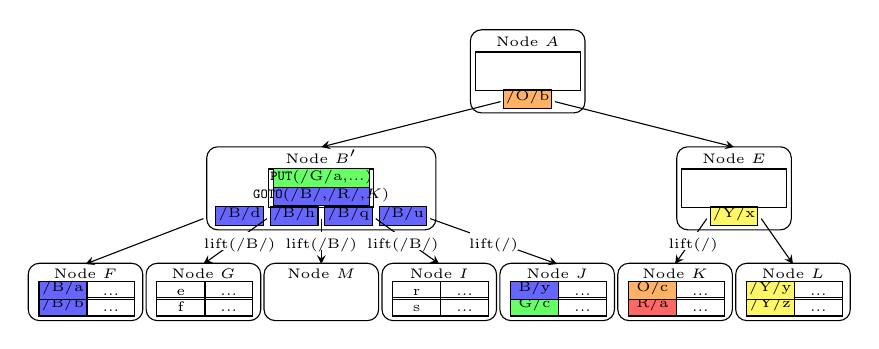
\begin{tikzpicture}[xscale=0.95, yscale=0.95]
            \node[anchor=south, rectangle, rounded corners, minimum height=.06\textwidth, minimum width=.12\textwidth, draw=black] at (0, 0) {};
            \node[anchor=south, font=\tiny] at (0, .036\textwidth) {Node $F$};
            \node[anchor=south, rectangle, minimum height=.015\textwidth, minimum width=.05\textwidth, draw=black, fill={blue!60}] at (-.025\textwidth, .005\textwidth) {};
            \node[anchor=south, font=\tiny] at (-.025\textwidth, 0) {/B/b};
            \node[anchor=south, rectangle, minimum height=.015\textwidth, minimum width=.05\textwidth, draw=black] at (.028\textwidth, .005\textwidth) {};
            \node[anchor=south, font=\tiny] at (.028\textwidth, 0) {...};
            \node[anchor=south, rectangle, minimum height=.015\textwidth, minimum width=.05\textwidth, draw=black, fill={blue!60}] at (-.025\textwidth, .023\textwidth) {};
            \node[anchor=south, font=\tiny] at (-.025\textwidth, .018\textwidth) {/B/a};
            \node[anchor=south, rectangle, minimum height=.015\textwidth, minimum width=.05\textwidth, draw=black] at (.028\textwidth, .023\textwidth) {};
            \node[anchor=south, font=\tiny] at (.028\textwidth, .018\textwidth) {...};

            \node[anchor=south, rectangle, rounded corners, minimum height=.06\textwidth, minimum width=.12\textwidth, draw=black] at (.13\textwidth, 0) {};
            \node[anchor=south, font=\tiny] at (.13\textwidth, .036\textwidth) {Node $G$};
            \node[anchor=south, rectangle, minimum height=.015\textwidth, minimum width=.05\textwidth, draw=black] at (.105\textwidth, .005\textwidth) {};
            \node[anchor=south, font=\tiny] at (.105\textwidth, 0) {f};
            \node[anchor=south, rectangle, minimum height=.015\textwidth, minimum width=.05\textwidth, draw=black] at (.158\textwidth, .005\textwidth) {};
            \node[anchor=south, font=\tiny] at (.158\textwidth, 0) {...};
            \node[anchor=south, rectangle, minimum height=.015\textwidth, minimum width=.05\textwidth, draw=black] at (.105\textwidth, .023\textwidth) {};
            \node[anchor=south, font=\tiny] at (.105\textwidth, .018\textwidth) {e};
            \node[anchor=south, rectangle, minimum height=.015\textwidth, minimum width=.05\textwidth, draw=black] at (.158\textwidth, .023\textwidth) {};
            \node[anchor=south, font=\tiny] at (.158\textwidth, .018\textwidth) {...};

            \node[anchor=south, rectangle, rounded corners, minimum height=.06\textwidth, minimum width=.12\textwidth, draw=black] at (.26\textwidth, 0) {};
            \node[anchor=south, font=\tiny] at (.26\textwidth, .036\textwidth) {Node $M$};

            \node[anchor=south, rectangle, rounded corners, minimum height=.06\textwidth, minimum width=.12\textwidth, draw=black] at (.39\textwidth, 0) {};
            \node[anchor=south, font=\tiny] at (.39\textwidth, .036\textwidth) {Node $I$};
            \node[anchor=south, rectangle, minimum height=.015\textwidth, minimum width=.05\textwidth, draw=black] at (.365\textwidth, .005\textwidth) {};
            \node[anchor=south, font=\tiny] at (.365\textwidth, 0) {s};
            \node[anchor=south, rectangle, minimum height=.015\textwidth, minimum width=.05\textwidth, draw=black] at (.418\textwidth, .005\textwidth) {};
            \node[anchor=south, font=\tiny] at (.418\textwidth, 0) {...};
            \node[anchor=south, rectangle, minimum height=.015\textwidth, minimum width=.05\textwidth, draw=black] at (.365\textwidth, .023\textwidth) {};
            \node[anchor=south, font=\tiny] at (.365\textwidth, .018\textwidth) {r};
            \node[anchor=south, rectangle, minimum height=.015\textwidth, minimum width=.05\textwidth, draw=black] at (.418\textwidth, .023\textwidth) {};
            \node[anchor=south, font=\tiny] at (.418\textwidth, .018\textwidth) {...};

            \node[anchor=south, rectangle, rounded corners, minimum height=.06\textwidth, minimum width=.12\textwidth, draw=black] at (.52\textwidth, 0) {};
            \node[anchor=south, font=\tiny] at (.52\textwidth, .036\textwidth) {Node $J$};
            \node[anchor=south, rectangle, minimum height=.015\textwidth, minimum width=.05\textwidth, draw=black, fill={green!60}] at (.495\textwidth, .005\textwidth) {};
            \node[anchor=south, font=\tiny] at (.495\textwidth, 0) {G/c};
            \node[anchor=south, rectangle, minimum height=.015\textwidth, minimum width=.05\textwidth, draw=black] at (.548\textwidth, .005\textwidth) {};
            \node[anchor=south, font=\tiny] at (.548\textwidth, 0) {...};
            \node[anchor=south, rectangle, minimum height=.015\textwidth, minimum width=.05\textwidth, draw=black, fill={blue!60}] at (.495\textwidth, .023\textwidth) {};
            \node[anchor=south, font=\tiny] at (.495\textwidth, .018\textwidth) {B/y};
            \node[anchor=south, rectangle, minimum height=.015\textwidth, minimum width=.05\textwidth, draw=black] at (.548\textwidth, .023\textwidth) {};
            \node[anchor=south, font=\tiny] at (.548\textwidth, .018\textwidth) {...};

            \node[anchor=south, rectangle, rounded corners, minimum height=.06\textwidth, minimum width=.12\textwidth, draw=black] at (.65\textwidth, 0) {};
            \node[anchor=south, font=\tiny] at (.65\textwidth, .036\textwidth) {Node $K$};
            \node[anchor=south, rectangle, minimum height=.015\textwidth, minimum width=.05\textwidth, draw=black, fill={red!60}] at (.625\textwidth, .005\textwidth) {};
            \node[anchor=south, font=\tiny] at (.625\textwidth, 0) {R/a};
            \node[anchor=south, rectangle, minimum height=.015\textwidth, minimum width=.05\textwidth, draw=black] at (.678\textwidth, .005\textwidth) {};
            \node[anchor=south, font=\tiny] at (.678\textwidth, 0) {...};
            \node[anchor=south, rectangle, minimum height=.015\textwidth, minimum width=.05\textwidth, draw=black, fill={orange!60}] at (.625\textwidth, .023\textwidth) {};
            \node[anchor=south, font=\tiny] at (.625\textwidth, .018\textwidth) {O/c};
            \node[anchor=south, rectangle, minimum height=.015\textwidth, minimum width=.05\textwidth, draw=black] at (.678\textwidth, .023\textwidth) {};
            \node[anchor=south, font=\tiny] at (.678\textwidth, .018\textwidth) {...};

            \node[anchor=south, rectangle, rounded corners, minimum height=.06\textwidth, minimum width=.12\textwidth, draw=black] at (.78\textwidth, 0) {};
            \node[anchor=south, font=\tiny] at (.78\textwidth, .036\textwidth) {Node $L$};
            \node[anchor=south, rectangle, minimum height=.015\textwidth, minimum width=.05\textwidth, draw=black, fill={yellow!60}] at (.755\textwidth, .005\textwidth) {};
            \node[anchor=south, font=\tiny] at (.755\textwidth, 0) {/Y/z};
            \node[anchor=south, rectangle, minimum height=.015\textwidth, minimum width=.05\textwidth, draw=black] at (.808\textwidth, .005\textwidth) {};
            \node[anchor=south, font=\tiny] at (.808\textwidth, 0) {...};
            \node[anchor=south, rectangle, minimum height=.015\textwidth, minimum width=.05\textwidth, draw=black, fill={yellow!60}] at (.755\textwidth, .023\textwidth) {};
            \node[anchor=south, font=\tiny] at (.755\textwidth, .018\textwidth) {/Y/y};
            \node[anchor=south, rectangle, minimum height=.015\textwidth, minimum width=.05\textwidth, draw=black] at (.808\textwidth, .023\textwidth) {};
            \node[anchor=south, font=\tiny] at (.808\textwidth, .018\textwidth) {...};

            \node[anchor=south, rectangle, rounded corners, minimum height=.087\textwidth, minimum width=.24\textwidth, draw=black] at (.26\textwidth, .1\textwidth) {};
            \node[anchor=south, font=\tiny] at (.26\textwidth, .163\textwidth) {Node $B'$};
            \node[anchor=south, rectangle, minimum height=.015\textwidth, minimum width=.05\textwidth, draw=black, fill={blue!60}] at (.17\textwidth, .105\textwidth) {};
            \node[anchor=south, font=\tiny] at (.17\textwidth, .1\textwidth) {/B/d};
            \node[anchor=south, rectangle, minimum height=.015\textwidth, minimum width=.05\textwidth, draw=black, fill={blue!60}] at (.23\textwidth, .105\textwidth) {};
            \node[anchor=south, font=\tiny] at (.23\textwidth, .1\textwidth) {/B/h};
            \node[anchor=south, rectangle, minimum height=.015\textwidth, minimum width=.05\textwidth, draw=black, fill={blue!60}] at (.29\textwidth, .105\textwidth) {};
            \node[anchor=south, font=\tiny] at (.29\textwidth, .1\textwidth) {/B/q};
            \node[anchor=south, rectangle, minimum height=.015\textwidth, minimum width=.05\textwidth, draw=black, fill={blue!60}] at (.35\textwidth, .105\textwidth) {};
            \node[anchor=south, font=\tiny] at (.35\textwidth, .1\textwidth) {/B/u};
            \node[anchor=south, rectangle, minimum height=.04\textwidth, minimum width=.11\textwidth, draw=black] at (.26\textwidth, .125\textwidth) {};
            \node[anchor=south, rectangle, minimum height=.015\textwidth, minimum width=.1\textwidth, draw=black, fill={blue!60}] at (.26\textwidth, .127\textwidth) {};
            \node[anchor=south, font=\tiny] at  (.26\textwidth, .121\textwidth) {\goto(/B/,/R/,$K$)};
            \node[anchor=south, rectangle, minimum height=.015\textwidth, minimum width=.1\textwidth, draw=black, fill={green!60}] at (.26\textwidth, .147\textwidth) {};
            \node[anchor=south, font=\tiny] at  (.26\textwidth, .141\textwidth) {\putm(/G/a,...)};

            \node[anchor=south, rectangle, rounded corners, minimum height=.087\textwidth, minimum width=.12\textwidth, draw=black] at (.715\textwidth, .1\textwidth) {};
            \node[anchor=south, font=\tiny] at (.715\textwidth, .163\textwidth) {Node $E$};
            \node[anchor=south, rectangle, minimum height=.015\textwidth, minimum width=.05\textwidth, draw=black, fill={yellow!60}] at (.715\textwidth, .105\textwidth) {};
            \node[anchor=south, font=\tiny] at (.715\textwidth, .1\textwidth) {/Y/x};
            \node[anchor=south, rectangle, minimum height=.04\textwidth, minimum width=.11\textwidth, draw=black] at (.715\textwidth, .125\textwidth) {};

            \node[anchor=south, rectangle, rounded corners, minimum height=.087\textwidth, minimum width=.12\textwidth, draw=black] at (.4875\textwidth, .229\textwidth) {};
            \node[anchor=south, font=\tiny] at (.4875\textwidth, .292\textwidth) {Node $A$};
            \node[anchor=south, rectangle, minimum height=.015\textwidth, minimum width=.05\textwidth, draw=black, fill={orange!60}] at (.4875\textwidth, .234\textwidth) {};
            \node[anchor=south, font=\tiny] at (.4875\textwidth, .229\textwidth) {/O/b};
            \node[anchor=south, rectangle, minimum height=.04\textwidth, minimum width=.11\textwidth, draw=black] at (.4875\textwidth, .254\textwidth) {};

            \draw[->, >=stealth] (.13\textwidth, .113\textwidth) -- (0, .063\textwidth);
            \draw[->, >=stealth] (.20\textwidth, .113\textwidth) -- (.13\textwidth, .063\textwidth);
            \draw[->, >=stealth] (.26\textwidth, .113\textwidth) -- (.26\textwidth, .063\textwidth);
            \draw[->, >=stealth] (.32\textwidth, .113\textwidth) -- (.39\textwidth, .063\textwidth);
            \draw[->, >=stealth] (.38\textwidth, .113\textwidth) -- (.52\textwidth, .063\textwidth);
            \draw[->, >=stealth] (.685\textwidth, .113\textwidth) -- (.65\textwidth, .063\textwidth);
            \draw[->, >=stealth] (.745\textwidth, .113\textwidth) -- (.78\textwidth, .063\textwidth);
            \draw[->, >=stealth] (.4575\textwidth, .242\textwidth) -- (.26\textwidth, .192\textwidth);
            \draw[->, >=stealth] (.5175\textwidth, .242\textwidth) -- (.715\textwidth, .192\textwidth);

            \node[anchor=north,rectangle, minimum height=.015\textwidth, minimum width=.05\textwidth, fill={white}] at (.17\textwidth, .099\textwidth) {};
            \node[anchor=north, font=\tiny] at (.17\textwidth, .102\textwidth) {lift(/B/)};
            \node[anchor=north,rectangle, minimum height=.015\textwidth, minimum width=.05\textwidth, fill={white}] at (.26\textwidth, .099\textwidth) {};
            \node[anchor=north, font=\tiny] at (.26\textwidth, .102\textwidth) {lift(/B/)};
            \node[anchor=north,rectangle, minimum height=.015\textwidth, minimum width=.05\textwidth, fill={white}] at (.35\textwidth, .099\textwidth) {};
            \node[anchor=north, font=\tiny] at (.35\textwidth, .102\textwidth) {lift(/B/)};
            \node[anchor=north,rectangle, minimum height=.015\textwidth, minimum width=.05\textwidth, fill={white}] at (.45\textwidth, .099\textwidth) {};
            \node[anchor=north, font=\tiny] at (.45\textwidth, .102\textwidth) {lift(/)};
            \node[anchor=north,rectangle, minimum height=.015\textwidth, minimum width=.05\textwidth, fill={white}] at (.67\textwidth, .099\textwidth) {};
            \node[anchor=north, font=\tiny] at (.67\textwidth, .102\textwidth) {lift(/)};
        \end{tikzpicture}
        \caption{\label{subfig:flush-2} The lifted \bedag garbage-collects Node
            $C$ and merges Node $B$ and $D$ into Node $B'$,
            which can accommodate the \goto message.}
    \end{subfigure}
    \caption[The \bedag merges children before flushing a \goto message]{\label{fig:flush}
        When a node tries to flush a \goto message, there may be more than
        one child that overlaps with the key range of the \goto message.
        In this case, the \bedag must merge children to create a single child
        that can accommodate the \goto message.}
\end{figure}


In the more complicated case, a \goto message can overlap with the key ranges
of multiple children.
There are at most two fringe children whose key ranges are partly covered by the
key range of the \goto message,
and partly out of the key range of the \goto message;
there are also some interior children whose key ranges are entirely
within the key range occluded by the \goto message.
The lift \bedag needs to create a single child that can accommodate the \goto
message.

To this end, the \bedag removes the references and pointers to the
interior children (potentially garbage-collecting these nodes, if this is
the last reference),
and merges the two fringe children into one child.
Removing interior children creates a key range that is not covered by the
fringe children.
One solution is to expand the key range of one fringe child,
however, changing the key range of a node means re-lifting the node and at
least one descendant at each height.
To avoid touching any descendant of the fringe children,
we add an empty subtree that covers the key range as the child of the merged
node.

Figure~\ref{fig:flush} shows an example of merging children before flushing a
\goto message.
In Figure~\ref{subfig:flush-1}, Node $B$, $C$ and $D$ all overlaps with the
range of the \goto message.
Node $B$ AND $D$ are fringe children, while Node $C$ is an interior child.
To flush the \goto message, in Figure~\ref{subfig:flush-2}, the lifted \bedag
garbage-collects Node $C$ and merges Node $B$ and $D$ into Node $B'$.
After the merge, Node $A$ flushes the \goto message to Node $B'$.
Note in the example, the merge creates an empty node, Node $M$, to cover the key
range (``/B/h'', ``/B/q'').

In special cases, there can be only one or no fringe child.
If there is only one fringe child, we removes the interior children and add
an empty subtree to cover the key range as one child of the fringe child.
If there is no fringe child, we remove the interior child and add an empty
subtree to cover the key range as the child of the node.

\paragraph{Converting \goto messages to pivots and parent-to-child pointers.}
After the merging process, there is only one child whose key range overlaps
with the key range of the \goto message.
If the child is higher than the source LCA of the \goto message,
we can simple flush the \goto message to the child buffer.
However, if the child is at the same height as the source LCA,
we cannot flush the \goto message.
Otherwise, the \goto message would redirect queries to a node at the same level,
which breaks the asymptotic I/O costs of queries.

In such scenarios, the \goto message is converted into into pivots and a
parent-to-child pointer in the node.

This is done by adding \dpre$_{min}$ and \dpre$_{max}$ as two new pivots and
set the parent-to-child pointer between the two pivots to the source LCA of the
\goto message.
Assume \dpre$_{min}$ and \dpre$_{max}$ are in the range of child $i$ of the node,
i.e., $\dpre_{min}, \dpre_{max} \in (pivot_{i},pivot_{i+1})$.
Adding \dpre$_{min}$ and \dpre$_{max}$ as two new pivots creates 3 key ranges,
$(pivot_{i},\dpre_{min})$, $(\dpre_{min},\dpre_{max})$ and
$(\dpre_{max}, pivot_{i+1})$.
Key range $(\dpre_{min},\dpre_{max})$ is cover in the source LCA of the \goto
message, while the other two are covered by child $i$.

However, all three parent-to-child pointers now points to a child whose key
range is different than those specified in the node.
In particular, child $i$ has range $(pivot_{i},pivot_{i+1})$ but bounded by
$(pivot_{i},\dpre_{min})$ or $(\dpre_{max}, pivot_{i+1})$.
The source LCA has a key range that might be larger than
$(\spre_{min}, \spre_{max})$ but bounded by $(\dpre_{min},\dpre_{max})$.
A smaller key range may lift a longer prefix through the parent-to-child
pointer.

The problem is solved by augmenting parent-to-child pointers with \xf functions,
which is the same as the \xf function described in \goto messages.
Each parent-to-child pointer now has a \xf function with a prefix.
After the query lifts its search key by the LCP of two pivots, the \xf function
prepends its prefix to the search key.
Also, \xf functions serves as filters, bounding the results queries may return.

\begin{figure}
    \begin{subfigure}{\textwidth}
        \centering
        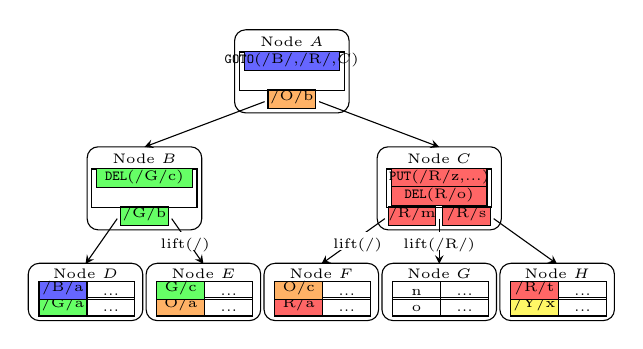
\begin{tikzpicture}[xscale=0.95, yscale=0.95]
            \node[anchor=south, rectangle, rounded corners, minimum height=.06\textwidth, minimum width=.12\textwidth, draw=black] at (0, 0) {};
            \node[anchor=south, font=\tiny] at (0, .036\textwidth) {Node $F$};
            \node[anchor=south, rectangle, minimum height=.015\textwidth, minimum width=.05\textwidth, draw=black, fill={red!60}] at (-.025\textwidth, .005\textwidth) {};
            \node[anchor=south, font=\tiny] at (-.025\textwidth, 0) {R/a};
            \node[anchor=south, rectangle, minimum height=.015\textwidth, minimum width=.05\textwidth, draw=black] at (.028\textwidth, .005\textwidth) {};
            \node[anchor=south, font=\tiny] at (.028\textwidth, 0) {...};
            \node[anchor=south, rectangle, minimum height=.015\textwidth, minimum width=.05\textwidth, draw=black, fill={orange!60}] at (-.025\textwidth, .023\textwidth) {};
            \node[anchor=south, font=\tiny] at (-.025\textwidth, .018\textwidth) {O/c};
            \node[anchor=south, rectangle, minimum height=.015\textwidth, minimum width=.05\textwidth, draw=black] at (.028\textwidth, .023\textwidth) {};
            \node[anchor=south, font=\tiny] at (.028\textwidth, .018\textwidth) {...};

            \node[anchor=south, rectangle, rounded corners, minimum height=.06\textwidth, minimum width=.12\textwidth, draw=black] at (.13\textwidth, 0) {};
            \node[anchor=south, font=\tiny] at (.13\textwidth, .036\textwidth) {Node $G$};
            \node[anchor=south, rectangle, minimum height=.015\textwidth, minimum width=.05\textwidth, draw=black] at (.105\textwidth, .005\textwidth) {};
            \node[anchor=south, font=\tiny] at (.105\textwidth, 0) {o};
            \node[anchor=south, rectangle, minimum height=.015\textwidth, minimum width=.05\textwidth, draw=black] at (.158\textwidth, .005\textwidth) {};
            \node[anchor=south, font=\tiny] at (.158\textwidth, 0) {...};
            \node[anchor=south, rectangle, minimum height=.015\textwidth, minimum width=.05\textwidth, draw=black] at (.105\textwidth, .023\textwidth) {};
            \node[anchor=south, font=\tiny] at (.105\textwidth, .018\textwidth) {n};
            \node[anchor=south, rectangle, minimum height=.015\textwidth, minimum width=.05\textwidth, draw=black] at (.158\textwidth, .023\textwidth) {};
            \node[anchor=south, font=\tiny] at (.158\textwidth, .018\textwidth) {...};

            \node[anchor=south, rectangle, rounded corners, minimum height=.06\textwidth, minimum width=.12\textwidth, draw=black] at (.26\textwidth, 0) {};
            \node[anchor=south, font=\tiny] at (.26\textwidth, .036\textwidth) {Node $H$};
            \node[anchor=south, rectangle, minimum height=.015\textwidth, minimum width=.05\textwidth, draw=black, fill={yellow!60}] at (.235\textwidth, .005\textwidth) {};
            \node[anchor=south, font=\tiny] at (.235\textwidth, 0) {/Y/x};
            \node[anchor=south, rectangle, minimum height=.015\textwidth, minimum width=.05\textwidth, draw=black] at (.288\textwidth, .005\textwidth) {};
            \node[anchor=south, font=\tiny] at (.288\textwidth, 0) {...};
            \node[anchor=south, rectangle, minimum height=.015\textwidth, minimum width=.05\textwidth, draw=black, fill={red!60}] at (.235\textwidth, .023\textwidth) {};
            \node[anchor=south, font=\tiny] at (.235\textwidth, .018\textwidth) {/R/t};
            \node[anchor=south, rectangle, minimum height=.015\textwidth, minimum width=.05\textwidth, draw=black] at (.288\textwidth, .023\textwidth) {};
            \node[anchor=south, font=\tiny] at (.288\textwidth, .018\textwidth) {...};

            \node[anchor=south, rectangle, rounded corners, minimum height=.06\textwidth, minimum width=.12\textwidth, draw=black] at (-.13\textwidth, 0) {};
            \node[anchor=south, font=\tiny] at (-.13\textwidth, .036\textwidth) {Node $E$};
            \node[anchor=south, rectangle, minimum height=.015\textwidth, minimum width=.05\textwidth, draw=black, fill={orange!60}] at (-.155\textwidth, .005\textwidth) {};
            \node[anchor=south, font=\tiny] at (-.155\textwidth, 0) {O/a};
            \node[anchor=south, rectangle, minimum height=.015\textwidth, minimum width=.05\textwidth, draw=black] at (-.102\textwidth, .005\textwidth) {};
            \node[anchor=south, font=\tiny] at (-.102\textwidth, 0) {...};
            \node[anchor=south, rectangle, minimum height=.015\textwidth, minimum width=.05\textwidth, draw=black, fill={green!60}] at (-.155\textwidth, .023\textwidth) {};
            \node[anchor=south, font=\tiny] at (-.155\textwidth, .018\textwidth) {G/c};
            \node[anchor=south, rectangle, minimum height=.015\textwidth, minimum width=.05\textwidth, draw=black] at (-.102\textwidth, .023\textwidth) {};
            \node[anchor=south, font=\tiny] at (-.102\textwidth, .018\textwidth) {...};

            \node[anchor=south, rectangle, rounded corners, minimum height=.06\textwidth, minimum width=.12\textwidth, draw=black] at (-.26\textwidth, 0) {};
            \node[anchor=south, font=\tiny] at (-.26\textwidth, .036\textwidth) {Node $D$};
            \node[anchor=south, rectangle, minimum height=.015\textwidth, minimum width=.05\textwidth, draw=black, fill={green!60}] at (-.285\textwidth, .005\textwidth) {};
            \node[anchor=south, font=\tiny] at (-.285\textwidth, 0) {/G/a};
            \node[anchor=south, rectangle, minimum height=.015\textwidth, minimum width=.05\textwidth, draw=black] at (-.232\textwidth, .005\textwidth) {};
            \node[anchor=south, font=\tiny] at (-.232\textwidth, 0) {...};
            \node[anchor=south, rectangle, minimum height=.015\textwidth, minimum width=.05\textwidth, draw=black, fill={blue!60}] at (-.285\textwidth, .023\textwidth) {};
            \node[anchor=south, font=\tiny] at (-.285\textwidth, .018\textwidth) {/B/a};
            \node[anchor=south, rectangle, minimum height=.015\textwidth, minimum width=.05\textwidth, draw=black] at (-.232\textwidth, .023\textwidth) {};
            \node[anchor=south, font=\tiny] at (-.232\textwidth, .018\textwidth) {...};

            \node[anchor=south, rectangle, rounded corners, minimum height=.087\textwidth, minimum width=.12\textwidth, draw=black] at (-.195\textwidth, .1\textwidth) {};
            \node[anchor=south, font=\tiny] at (-.195\textwidth, .163\textwidth) {Node $B$};
            \node[anchor=south, rectangle, minimum height=.015\textwidth, minimum width=.05\textwidth, draw=black, fill={green!60}] at (-.195\textwidth, .105\textwidth) {};
            \node[anchor=south, font=\tiny] at (-.195\textwidth, .1\textwidth) {/G/b};
            \node[anchor=south, rectangle, minimum height=.04\textwidth, minimum width=.11\textwidth, draw=black] at (-.195\textwidth, .125\textwidth) {};
            \node[anchor=south, rectangle, minimum height=.015\textwidth, minimum width=.1\textwidth, draw=black, fill={green!60}] at (-.195\textwidth, .147\textwidth) {};
            \node[anchor=south, font=\tiny] at  (-.195\textwidth, .141\textwidth) {\delm(/G/c)};

            \node[anchor=south, rectangle, rounded corners, minimum height=.087\textwidth, minimum width=.13\textwidth, draw=black] at (.13\textwidth, .1\textwidth) {};
            \node[anchor=south, font=\tiny] at (.13\textwidth, .163\textwidth) {Node $C$};
            \node[anchor=south, rectangle, minimum height=.015\textwidth, minimum width=.05\textwidth, draw=black, fill={red!60}] at (.1\textwidth, .105\textwidth) {};
            \node[anchor=south, font=\tiny] at (.1\textwidth, .1\textwidth) {/R/m};
            \node[anchor=south, rectangle, minimum height=.015\textwidth, minimum width=.05\textwidth, draw=black, fill={red!60}] at (.16\textwidth, .105\textwidth) {};
            \node[anchor=south, font=\tiny] at (.16\textwidth, .1\textwidth) {/R/s};
            \node[anchor=south, rectangle, minimum height=.04\textwidth, minimum width=.11\textwidth, draw=black] at (.13\textwidth, .125\textwidth) {};
            \node[anchor=south, rectangle, minimum height=.015\textwidth, minimum width=.1\textwidth, draw=black, fill={red!60}] at (.13\textwidth, .147\textwidth) {};
            \node[anchor=south, font=\tiny] at  (.13\textwidth, .141\textwidth) {\putm(/R/z,...)};
            \node[anchor=south, rectangle, minimum height=.015\textwidth, minimum width=.1\textwidth, draw=black, fill={red!60}] at (.13\textwidth, .127\textwidth) {};
            \node[anchor=south, font=\tiny] at  (.13\textwidth, .121\textwidth) {\delm(R/o)};

            \node[anchor=south, rectangle, rounded corners, minimum height=.087\textwidth, minimum width=.12\textwidth, draw=black] at (-.0325\textwidth, .229\textwidth) {};
            \node[anchor=south, font=\tiny] at (-.0325\textwidth, .292\textwidth) {Node $A$};
            \node[anchor=south, rectangle, minimum height=.015\textwidth, minimum width=.05\textwidth, draw=black, fill={orange!60}] at (-.0325\textwidth, .234\textwidth) {};
            \node[anchor=south, font=\tiny] at (-.0325\textwidth, .229\textwidth) {/O/b};
            \node[anchor=south, rectangle, minimum height=.04\textwidth, minimum width=.11\textwidth, draw=black] at (-.0325\textwidth, .254\textwidth) {};
            \node[anchor=south, rectangle, minimum height=.015\textwidth, minimum width=.1\textwidth, draw=black, fill={blue!60}] at (-.0325\textwidth, .276\textwidth) {};
            \node[anchor=south, font=\tiny] at  (-.0325\textwidth, .27\textwidth) {\goto(/B/,/R/,$C$)};

            \draw[->, >=stealth] (-.225\textwidth, .113\textwidth) -- (-.26\textwidth, .063\textwidth);
            \draw[->, >=stealth] (-.165\textwidth, .113\textwidth) -- (-.13\textwidth, .063\textwidth);
            \draw[->, >=stealth] (.13\textwidth, .113\textwidth) -- (.13\textwidth, .063\textwidth);
            \draw[->, >=stealth] (.19\textwidth, .113\textwidth) -- (.26\textwidth, .063\textwidth);
            \draw[->, >=stealth] (.07\textwidth, .113\textwidth) -- (0, .063\textwidth);
            \draw[->, >=stealth] (-.0625\textwidth, .242\textwidth) -- (-.195\textwidth, .192\textwidth);
            \draw[->, >=stealth] (-.0025\textwidth, .242\textwidth) -- (.13\textwidth, .192\textwidth);

            \node[anchor=north,rectangle, minimum height=.015\textwidth, minimum width=.05\textwidth, fill={white}] at (.13\textwidth, .099\textwidth) {};
            \node[anchor=north, font=\tiny] at (.13\textwidth, .102\textwidth) {lift(/R/)};
            \node[anchor=north,rectangle, minimum height=.015\textwidth, minimum width=.05\textwidth, fill={white}] at (.04\textwidth, .099\textwidth) {};
            \node[anchor=north, font=\tiny] at (.04\textwidth, .102\textwidth) {lift(/)};
            \node[anchor=north,rectangle, minimum height=.015\textwidth, minimum width=.05\textwidth, fill={white}] at (-.15\textwidth, .099\textwidth) {};
            \node[anchor=north, font=\tiny] at (-.15\textwidth, .102\textwidth) {lift(/)};
        \end{tikzpicture}
        \caption{\label{subfig:spvt-1} The \goto message cannot be flushed to
            Node $B$, which is at the same as Node $C$.}
    \end{subfigure}
    \begin{subfigure}{\textwidth}
        \centering
        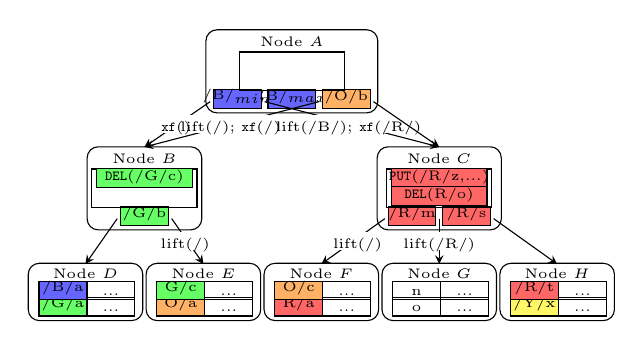
\begin{tikzpicture}[xscale=0.95, yscale=0.95]
            \node[anchor=south, rectangle, rounded corners, minimum height=.06\textwidth, minimum width=.12\textwidth, draw=black] at (0, 0) {};
            \node[anchor=south, font=\tiny] at (0, .036\textwidth) {Node $F$};
            \node[anchor=south, rectangle, minimum height=.015\textwidth, minimum width=.05\textwidth, draw=black, fill={red!60}] at (-.025\textwidth, .005\textwidth) {};
            \node[anchor=south, font=\tiny] at (-.025\textwidth, 0) {R/a};
            \node[anchor=south, rectangle, minimum height=.015\textwidth, minimum width=.05\textwidth, draw=black] at (.028\textwidth, .005\textwidth) {};
            \node[anchor=south, font=\tiny] at (.028\textwidth, 0) {...};
            \node[anchor=south, rectangle, minimum height=.015\textwidth, minimum width=.05\textwidth, draw=black, fill={orange!60}] at (-.025\textwidth, .023\textwidth) {};
            \node[anchor=south, font=\tiny] at (-.025\textwidth, .018\textwidth) {O/c};
            \node[anchor=south, rectangle, minimum height=.015\textwidth, minimum width=.05\textwidth, draw=black] at (.028\textwidth, .023\textwidth) {};
            \node[anchor=south, font=\tiny] at (.028\textwidth, .018\textwidth) {...};

            \node[anchor=south, rectangle, rounded corners, minimum height=.06\textwidth, minimum width=.12\textwidth, draw=black] at (.13\textwidth, 0) {};
            \node[anchor=south, font=\tiny] at (.13\textwidth, .036\textwidth) {Node $G$};
            \node[anchor=south, rectangle, minimum height=.015\textwidth, minimum width=.05\textwidth, draw=black] at (.105\textwidth, .005\textwidth) {};
            \node[anchor=south, font=\tiny] at (.105\textwidth, 0) {o};
            \node[anchor=south, rectangle, minimum height=.015\textwidth, minimum width=.05\textwidth, draw=black] at (.158\textwidth, .005\textwidth) {};
            \node[anchor=south, font=\tiny] at (.158\textwidth, 0) {...};
            \node[anchor=south, rectangle, minimum height=.015\textwidth, minimum width=.05\textwidth, draw=black] at (.105\textwidth, .023\textwidth) {};
            \node[anchor=south, font=\tiny] at (.105\textwidth, .018\textwidth) {n};
            \node[anchor=south, rectangle, minimum height=.015\textwidth, minimum width=.05\textwidth, draw=black] at (.158\textwidth, .023\textwidth) {};
            \node[anchor=south, font=\tiny] at (.158\textwidth, .018\textwidth) {...};

            \node[anchor=south, rectangle, rounded corners, minimum height=.06\textwidth, minimum width=.12\textwidth, draw=black] at (.26\textwidth, 0) {};
            \node[anchor=south, font=\tiny] at (.26\textwidth, .036\textwidth) {Node $H$};
            \node[anchor=south, rectangle, minimum height=.015\textwidth, minimum width=.05\textwidth, draw=black, fill={yellow!60}] at (.235\textwidth, .005\textwidth) {};
            \node[anchor=south, font=\tiny] at (.235\textwidth, 0) {/Y/x};
            \node[anchor=south, rectangle, minimum height=.015\textwidth, minimum width=.05\textwidth, draw=black] at (.288\textwidth, .005\textwidth) {};
            \node[anchor=south, font=\tiny] at (.288\textwidth, 0) {...};
            \node[anchor=south, rectangle, minimum height=.015\textwidth, minimum width=.05\textwidth, draw=black, fill={red!60}] at (.235\textwidth, .023\textwidth) {};
            \node[anchor=south, font=\tiny] at (.235\textwidth, .018\textwidth) {/R/t};
            \node[anchor=south, rectangle, minimum height=.015\textwidth, minimum width=.05\textwidth, draw=black] at (.288\textwidth, .023\textwidth) {};
            \node[anchor=south, font=\tiny] at (.288\textwidth, .018\textwidth) {...};

            \node[anchor=south, rectangle, rounded corners, minimum height=.06\textwidth, minimum width=.12\textwidth, draw=black] at (-.13\textwidth, 0) {};
            \node[anchor=south, font=\tiny] at (-.13\textwidth, .036\textwidth) {Node $E$};
            \node[anchor=south, rectangle, minimum height=.015\textwidth, minimum width=.05\textwidth, draw=black, fill={orange!60}] at (-.155\textwidth, .005\textwidth) {};
            \node[anchor=south, font=\tiny] at (-.155\textwidth, 0) {O/a};
            \node[anchor=south, rectangle, minimum height=.015\textwidth, minimum width=.05\textwidth, draw=black] at (-.102\textwidth, .005\textwidth) {};
            \node[anchor=south, font=\tiny] at (-.102\textwidth, 0) {...};
            \node[anchor=south, rectangle, minimum height=.015\textwidth, minimum width=.05\textwidth, draw=black, fill={green!60}] at (-.155\textwidth, .023\textwidth) {};
            \node[anchor=south, font=\tiny] at (-.155\textwidth, .018\textwidth) {G/c};
            \node[anchor=south, rectangle, minimum height=.015\textwidth, minimum width=.05\textwidth, draw=black] at (-.102\textwidth, .023\textwidth) {};
            \node[anchor=south, font=\tiny] at (-.102\textwidth, .018\textwidth) {...};

            \node[anchor=south, rectangle, rounded corners, minimum height=.06\textwidth, minimum width=.12\textwidth, draw=black] at (-.26\textwidth, 0) {};
            \node[anchor=south, font=\tiny] at (-.26\textwidth, .036\textwidth) {Node $D$};
            \node[anchor=south, rectangle, minimum height=.015\textwidth, minimum width=.05\textwidth, draw=black, fill={green!60}] at (-.285\textwidth, .005\textwidth) {};
            \node[anchor=south, font=\tiny] at (-.285\textwidth, 0) {/G/a};
            \node[anchor=south, rectangle, minimum height=.015\textwidth, minimum width=.05\textwidth, draw=black] at (-.232\textwidth, .005\textwidth) {};
            \node[anchor=south, font=\tiny] at (-.232\textwidth, 0) {...};
            \node[anchor=south, rectangle, minimum height=.015\textwidth, minimum width=.05\textwidth, draw=black, fill={blue!60}] at (-.285\textwidth, .023\textwidth) {};
            \node[anchor=south, font=\tiny] at (-.285\textwidth, .018\textwidth) {/B/a};
            \node[anchor=south, rectangle, minimum height=.015\textwidth, minimum width=.05\textwidth, draw=black] at (-.232\textwidth, .023\textwidth) {};
            \node[anchor=south, font=\tiny] at (-.232\textwidth, .018\textwidth) {...};

            \node[anchor=south, rectangle, rounded corners, minimum height=.087\textwidth, minimum width=.12\textwidth, draw=black] at (-.195\textwidth, .1\textwidth) {};
            \node[anchor=south, font=\tiny] at (-.195\textwidth, .163\textwidth) {Node $B$};
            \node[anchor=south, rectangle, minimum height=.015\textwidth, minimum width=.05\textwidth, draw=black, fill={green!60}] at (-.195\textwidth, .105\textwidth) {};
            \node[anchor=south, font=\tiny] at (-.195\textwidth, .1\textwidth) {/G/b};
            \node[anchor=south, rectangle, minimum height=.04\textwidth, minimum width=.11\textwidth, draw=black] at (-.195\textwidth, .125\textwidth) {};
            \node[anchor=south, rectangle, minimum height=.015\textwidth, minimum width=.1\textwidth, draw=black, fill={green!60}] at (-.195\textwidth, .147\textwidth) {};
            \node[anchor=south, font=\tiny] at  (-.195\textwidth, .141\textwidth) {\delm(/G/c)};

            \node[anchor=south, rectangle, rounded corners, minimum height=.087\textwidth, minimum width=.13\textwidth, draw=black] at (.13\textwidth, .1\textwidth) {};
            \node[anchor=south, font=\tiny] at (.13\textwidth, .163\textwidth) {Node $C$};
            \node[anchor=south, rectangle, minimum height=.015\textwidth, minimum width=.05\textwidth, draw=black, fill={red!60}] at (.1\textwidth, .105\textwidth) {};
            \node[anchor=south, font=\tiny] at (.1\textwidth, .1\textwidth) {/R/m};
            \node[anchor=south, rectangle, minimum height=.015\textwidth, minimum width=.05\textwidth, draw=black, fill={red!60}] at (.16\textwidth, .105\textwidth) {};
            \node[anchor=south, font=\tiny] at (.16\textwidth, .1\textwidth) {/R/s};
            \node[anchor=south, rectangle, minimum height=.04\textwidth, minimum width=.11\textwidth, draw=black] at (.13\textwidth, .125\textwidth) {};
            \node[anchor=south, rectangle, minimum height=.015\textwidth, minimum width=.1\textwidth, draw=black, fill={red!60}] at (.13\textwidth, .147\textwidth) {};
            \node[anchor=south, font=\tiny] at  (.13\textwidth, .141\textwidth) {\putm(/R/z,...)};
            \node[anchor=south, rectangle, minimum height=.015\textwidth, minimum width=.1\textwidth, draw=black, fill={red!60}] at (.13\textwidth, .127\textwidth) {};
            \node[anchor=south, font=\tiny] at  (.13\textwidth, .121\textwidth) {\delm(R/o)};

            \node[anchor=south, rectangle, rounded corners, minimum height=.087\textwidth, minimum width=.18\textwidth, draw=black] at (-.0325\textwidth, .229\textwidth) {};
            \node[anchor=south, font=\tiny] at (-.0325\textwidth, .292\textwidth) {Node $A$};
            \node[anchor=south, rectangle, minimum height=.015\textwidth, minimum width=.05\textwidth, draw=black, fill={blue!60}] at (-.0325\textwidth, .234\textwidth) {};
            \node[anchor=south, font=\tiny] at (-.0325\textwidth, .229\textwidth) {/B/$_{max}$};
            \node[anchor=south, rectangle, minimum height=.015\textwidth, minimum width=.05\textwidth, draw=black, fill={blue!60}] at (-.0925\textwidth, .234\textwidth) {};
            \node[anchor=south, font=\tiny] at (-.0925\textwidth, .229\textwidth) {/B/$_{min}$};
            \node[anchor=south, rectangle, minimum height=.015\textwidth, minimum width=.05\textwidth, draw=black, fill={orange!60}] at (.0275\textwidth, .234\textwidth) {};
            \node[anchor=south, font=\tiny] at (.0275\textwidth, .229\textwidth) {/O/b};
            \node[anchor=south, rectangle, minimum height=.04\textwidth, minimum width=.11\textwidth, draw=black] at (-.0325\textwidth, .254\textwidth) {};

            \draw[->, >=stealth] (-.225\textwidth, .113\textwidth) -- (-.26\textwidth, .063\textwidth);
            \draw[->, >=stealth] (-.165\textwidth, .113\textwidth) -- (-.13\textwidth, .063\textwidth);
            \draw[->, >=stealth] (.13\textwidth, .113\textwidth) -- (.13\textwidth, .063\textwidth);
            \draw[->, >=stealth] (.19\textwidth, .113\textwidth) -- (.26\textwidth, .063\textwidth);
            \draw[->, >=stealth] (.07\textwidth, .113\textwidth) -- (0, .063\textwidth);
            \draw[->, >=stealth] (-.1225\textwidth, .242\textwidth) -- (-.195\textwidth, .192\textwidth);
            \draw[->, >=stealth] (-.0625\textwidth, .242\textwidth) -- (.13\textwidth, .192\textwidth);
            \draw[->, >=stealth] (-.0025\textwidth, .242\textwidth) -- (-.195\textwidth, .192\textwidth);
            \draw[->, >=stealth] (.0575\textwidth, .242\textwidth) -- (.13\textwidth, .192\textwidth);

            \node[anchor=north,rectangle, minimum height=.015\textwidth, minimum width=.05\textwidth, fill={white}] at (.13\textwidth, .099\textwidth) {};
            \node[anchor=north, font=\tiny] at (.13\textwidth, .102\textwidth) {lift(/R/)};
            \node[anchor=north,rectangle, minimum height=.015\textwidth, minimum width=.05\textwidth, fill={white}] at (.04\textwidth, .099\textwidth) {};
            \node[anchor=north, font=\tiny] at (.04\textwidth, .102\textwidth) {lift(/)};
            \node[anchor=north,rectangle, minimum height=.015\textwidth, minimum width=.05\textwidth, fill={white}] at (-.15\textwidth, .099\textwidth) {};
            \node[anchor=north, font=\tiny] at (-.15\textwidth, .102\textwidth) {lift(/)};
            \node[anchor=north,rectangle, minimum height=.015\textwidth, minimum width=.05\textwidth, fill={white}] at (-.16\textwidth, .228\textwidth) {};
            \node[anchor=north, font=\tiny] at (-.16\textwidth, .231\textwidth) {\xf ()};
            \node[anchor=north,rectangle, minimum height=.015\textwidth, minimum width=.08\textwidth, fill={white}] at (-.1\textwidth, .228\textwidth) {};
            \node[anchor=north, font=\tiny] at (-.1\textwidth, .231\textwidth) {lift(/); \xf (/)};
            \node[anchor=north,rectangle, minimum height=.015\textwidth, minimum width=.08\textwidth, fill={white}] at (.03\textwidth, .228\textwidth) {};
            \node[anchor=north, font=\tiny] at (.03\textwidth, .231\textwidth) {lift(/B/); \xf (/R/)};
        \end{tikzpicture}
        \caption{\label{subfig:spvt-2} The \goto message becomes pivots and a
            parent-to-child pointer, and adds \xf functions to the parent-to-child pointers.}
    \end{subfigure}
    \caption[Transform a \goto message into pivots and a parent-to-child pointer]{\label{fig:spvt}
        When the lifted \bedag cannot flush a \goto message deeper, it
        transforms the \goto message into pivots and a parent-to-child pointers
        and adds \xf functions to the parent-to-child pointers.}
\end{figure}

Figure~\ref{fig:spvt} shows an example of the transformation.
The lifted \bedag cannot flush the \goto message from Node $A$ to Node $B$,
because Node $B$ is at the same height as its source LCA, Node $C$.
Therefore, it adds two pivots, ``/B/$_{min}$'' and ``/B/$_{max}$'', to Node $A$.
The parent-to-child pointer between ``/B/$_{min}$'' and ``/B/$_{max}$'' points
to the source LCA, Node $C$, and has a \xf function of ``/R/'', indicating a
key range mismatch and the additional prefix ``/R/'' for keys in the child.
Queries following that parent-to-child pointer should prepend prefix ``/R/''
after the normal lifting of ``/B/'' from its search key.
Also, they remember only keys between ``/R/$_{min}$'' and ``/R/$_{max}$'' in
the child are valid.
Similarly, two \xf functions are added to the other two pointers.
Note, for the leftmost pointer, though the \xf function contains no prefix,
it still serves as a filter for queries.

\paragraph{Fixing \xf functions in parent-to-child pointers.}
\goto messages adds \xf functions to parent-to-child pointers.
The \xf function transforms the search keys of queries by prepending its prefix
after normal key lifting through parent-to-child pointers.
Also, the \xf function indicates the child contains keys outside of the key range
specified by pivots in the parent and queries should ignore those keys following
the parent-to-child pointers.

The lifted \bedag resolves \xf functions through node flushes.
Specifically, when flushing from a parent to a child and the parent-to-child
pointer has a \xf function,
the lifted \bedag garbage-collects exterior children of the child whose key
ranges are completely outside of the key range specified by the pivots in parent.
Also, the lifted \bedag removes messages whose keys are outside of the key
range specified in the parent from the child buffer.
Then, for fringe children whose key ranges partly overlaps with that specified
in the parent, the \bedag propagates the \xf function to their parent-to-child
pointers.
At last, if the \xf function has a prefix, the \bedag lifts the prefix from
keys in the child.

\begin{figure}
    \begin{subfigure}{\textwidth}
        \centering
        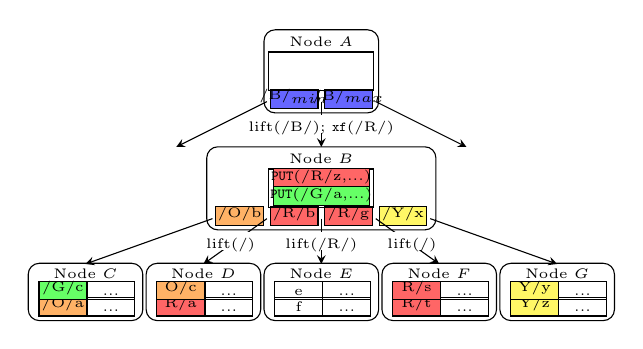
\begin{tikzpicture}[xscale=0.95, yscale=0.95]
            \node[anchor=south, rectangle, rounded corners, minimum height=.06\textwidth, minimum width=.12\textwidth, draw=black] at (0, 0) {};
            \node[anchor=south, font=\tiny] at (0, .036\textwidth) {Node $C$};
            \node[anchor=south, rectangle, minimum height=.015\textwidth, minimum width=.05\textwidth, draw=black, fill={orange!60}] at (-.025\textwidth, .005\textwidth) {};
            \node[anchor=south, font=\tiny] at (-.025\textwidth, 0) {/O/a};
            \node[anchor=south, rectangle, minimum height=.015\textwidth, minimum width=.05\textwidth, draw=black] at (.028\textwidth, .005\textwidth) {};
            \node[anchor=south, font=\tiny] at (.028\textwidth, 0) {...};
            \node[anchor=south, rectangle, minimum height=.015\textwidth, minimum width=.05\textwidth, draw=black, fill={green!60}] at (-.025\textwidth, .023\textwidth) {};
            \node[anchor=south, font=\tiny] at (-.025\textwidth, .018\textwidth) {/G/c};
            \node[anchor=south, rectangle, minimum height=.015\textwidth, minimum width=.05\textwidth, draw=black] at (.028\textwidth, .023\textwidth) {};
            \node[anchor=south, font=\tiny] at (.028\textwidth, .018\textwidth) {...};

            \node[anchor=south, rectangle, rounded corners, minimum height=.06\textwidth, minimum width=.12\textwidth, draw=black] at (.13\textwidth, 0) {};
            \node[anchor=south, font=\tiny] at (.13\textwidth, .036\textwidth) {Node $D$};
            \node[anchor=south, rectangle, minimum height=.015\textwidth, minimum width=.05\textwidth, draw=black, fill={red!60}] at (.105\textwidth, .005\textwidth) {};
            \node[anchor=south, font=\tiny] at (.105\textwidth, 0) {R/a};
            \node[anchor=south, rectangle, minimum height=.015\textwidth, minimum width=.05\textwidth, draw=black] at (.158\textwidth, .005\textwidth) {};
            \node[anchor=south, font=\tiny] at (.158\textwidth, 0) {...};
            \node[anchor=south, rectangle, minimum height=.015\textwidth, minimum width=.05\textwidth, draw=black, fill={orange!60}] at (.105\textwidth, .023\textwidth) {};
            \node[anchor=south, font=\tiny] at (.105\textwidth, .018\textwidth) {O/c};
            \node[anchor=south, rectangle, minimum height=.015\textwidth, minimum width=.05\textwidth, draw=black] at (.158\textwidth, .023\textwidth) {};
            \node[anchor=south, font=\tiny] at (.158\textwidth, .018\textwidth) {...};

            \node[anchor=south, rectangle, rounded corners, minimum height=.06\textwidth, minimum width=.12\textwidth, draw=black] at (.26\textwidth, 0) {};
            \node[anchor=south, font=\tiny] at (.26\textwidth, .036\textwidth) {Node $E$};
            \node[anchor=south, rectangle, minimum height=.015\textwidth, minimum width=.05\textwidth, draw=black] at (.235\textwidth, .005\textwidth) {};
            \node[anchor=south, font=\tiny] at (.235\textwidth, 0) {f};
            \node[anchor=south, rectangle, minimum height=.015\textwidth, minimum width=.05\textwidth, draw=black] at (.288\textwidth, .005\textwidth) {};
            \node[anchor=south, font=\tiny] at (.288\textwidth, 0) {...};
            \node[anchor=south, rectangle, minimum height=.015\textwidth, minimum width=.05\textwidth, draw=black] at (.235\textwidth, .023\textwidth) {};
            \node[anchor=south, font=\tiny] at (.235\textwidth, .018\textwidth) {e};
            \node[anchor=south, rectangle, minimum height=.015\textwidth, minimum width=.05\textwidth, draw=black] at (.288\textwidth, .023\textwidth) {};
            \node[anchor=south, font=\tiny] at (.288\textwidth, .018\textwidth) {...};

            \node[anchor=south, rectangle, rounded corners, minimum height=.06\textwidth, minimum width=.12\textwidth, draw=black] at (.39\textwidth, 0) {};
            \node[anchor=south, font=\tiny] at (.39\textwidth, .036\textwidth) {Node $F$};
            \node[anchor=south, rectangle, minimum height=.015\textwidth, minimum width=.05\textwidth, draw=black, fill={red!60}] at (.365\textwidth, .005\textwidth) {};
            \node[anchor=south, font=\tiny] at (.365\textwidth, 0) {R/t};
            \node[anchor=south, rectangle, minimum height=.015\textwidth, minimum width=.05\textwidth, draw=black] at (.418\textwidth, .005\textwidth) {};
            \node[anchor=south, font=\tiny] at (.418\textwidth, 0) {...};
            \node[anchor=south, rectangle, minimum height=.015\textwidth, minimum width=.05\textwidth, draw=black, fill={red!60}] at (.365\textwidth, .023\textwidth) {};
            \node[anchor=south, font=\tiny] at (.365\textwidth, .018\textwidth) {R/s};
            \node[anchor=south, rectangle, minimum height=.015\textwidth, minimum width=.05\textwidth, draw=black] at (.418\textwidth, .023\textwidth) {};
            \node[anchor=south, font=\tiny] at (.418\textwidth, .018\textwidth) {...};

            \node[anchor=south, rectangle, rounded corners, minimum height=.06\textwidth, minimum width=.12\textwidth, draw=black] at (.52\textwidth, 0) {};
            \node[anchor=south, font=\tiny] at (.52\textwidth, .036\textwidth) {Node $G$};
            \node[anchor=south, rectangle, minimum height=.015\textwidth, minimum width=.05\textwidth, draw=black, fill={yellow!60}] at (.495\textwidth, .005\textwidth) {};
            \node[anchor=south, font=\tiny] at (.495\textwidth, 0) {Y/z};
            \node[anchor=south, rectangle, minimum height=.015\textwidth, minimum width=.05\textwidth, draw=black] at (.548\textwidth, .005\textwidth) {};
            \node[anchor=south, font=\tiny] at (.548\textwidth, 0) {...};
            \node[anchor=south, rectangle, minimum height=.015\textwidth, minimum width=.05\textwidth, draw=black, fill={yellow!60}] at (.495\textwidth, .023\textwidth) {};
            \node[anchor=south, font=\tiny] at (.495\textwidth, .018\textwidth) {Y/y};
            \node[anchor=south, rectangle, minimum height=.015\textwidth, minimum width=.05\textwidth, draw=black] at (.548\textwidth, .023\textwidth) {};
            \node[anchor=south, font=\tiny] at (.548\textwidth, .018\textwidth) {...};

            \node[anchor=south, rectangle, rounded corners, minimum height=.087\textwidth, minimum width=.24\textwidth, draw=black] at (.26\textwidth, .1\textwidth) {};
            \node[anchor=south, font=\tiny] at (.26\textwidth, .163\textwidth) {Node $B$};
            \node[anchor=south, rectangle, minimum height=.015\textwidth, minimum width=.05\textwidth, draw=black, fill={orange!60}] at (.17\textwidth, .105\textwidth) {};
            \node[anchor=south, font=\tiny] at (.17\textwidth, .1\textwidth) {/O/b};
            \node[anchor=south, rectangle, minimum height=.015\textwidth, minimum width=.05\textwidth, draw=black, fill={red!60}] at (.23\textwidth, .105\textwidth) {};
            \node[anchor=south, font=\tiny] at (.23\textwidth, .1\textwidth) {/R/b};
            \node[anchor=south, rectangle, minimum height=.015\textwidth, minimum width=.05\textwidth, draw=black, fill={red!60}] at (.29\textwidth, .105\textwidth) {};
            \node[anchor=south, font=\tiny] at (.29\textwidth, .1\textwidth) {/R/g};
            \node[anchor=south, rectangle, minimum height=.015\textwidth, minimum width=.05\textwidth, draw=black, fill={yellow!60}] at (.35\textwidth, .105\textwidth) {};
            \node[anchor=south, font=\tiny] at (.35\textwidth, .1\textwidth) {/Y/x};
            \node[anchor=south, rectangle, minimum height=.04\textwidth, minimum width=.11\textwidth, draw=black] at (.26\textwidth, .125\textwidth) {};
            \node[anchor=south, rectangle, minimum height=.015\textwidth, minimum width=.1\textwidth, draw=black, fill={red!60}] at (.26\textwidth, .147\textwidth) {};
            \node[anchor=south, font=\tiny] at  (.26\textwidth, .141\textwidth) {\putm(/R/z,...)};
            \node[anchor=south, rectangle, minimum height=.015\textwidth, minimum width=.1\textwidth, draw=black, fill={green!60}] at (.26\textwidth, .127\textwidth) {};
            \node[anchor=south, font=\tiny] at  (.26\textwidth, .121\textwidth) {\putm(/G/a,...)};

            \node[anchor=south, rectangle, rounded corners, minimum height=.087\textwidth, minimum width=.12\textwidth, draw=black] at (.26\textwidth, .229\textwidth) {};
            \node[anchor=south, font=\tiny] at (.26\textwidth, .292\textwidth) {Node $A$};
            \node[anchor=south, rectangle, minimum height=.015\textwidth, minimum width=.05\textwidth, draw=black, fill={blue!60}] at (.23\textwidth, .234\textwidth) {};
            \node[anchor=south, font=\tiny] at (.23\textwidth, .229\textwidth) {/B/$_{min}$};
            \node[anchor=south, rectangle, minimum height=.015\textwidth, minimum width=.05\textwidth, draw=black, fill={blue!60}] at (.29\textwidth, .234\textwidth) {};
            \node[anchor=south, font=\tiny] at (.29\textwidth, .229\textwidth) {/B/$_{max}$};
            \node[anchor=south, rectangle, minimum height=.04\textwidth, minimum width=.11\textwidth, draw=black] at (.26\textwidth, .254\textwidth) {};

            \draw[->, >=stealth] (.14\textwidth, .113\textwidth) -- (0, .063\textwidth);
            \draw[->, >=stealth] (.20\textwidth, .113\textwidth) -- (.13\textwidth, .063\textwidth);
            \draw[->, >=stealth] (.26\textwidth, .113\textwidth) -- (.26\textwidth, .063\textwidth);
            \draw[->, >=stealth] (.32\textwidth, .113\textwidth) -- (.39\textwidth, .063\textwidth);
            \draw[->, >=stealth] (.38\textwidth, .113\textwidth) -- (.52\textwidth, .063\textwidth);
            \draw[->, >=stealth] (.26\textwidth, .242\textwidth) -- (.26\textwidth, .192\textwidth);
            \draw[->, >=stealth] (.20\textwidth, .242\textwidth) -- (.10\textwidth, .192\textwidth);
            \draw[->, >=stealth] (.32\textwidth, .242\textwidth) -- (.42\textwidth, .192\textwidth);

            \node[anchor=north,rectangle, minimum height=.015\textwidth, minimum width=.05\textwidth, fill={white}] at (.16\textwidth, .099\textwidth) {};
            \node[anchor=north, font=\tiny] at (.16\textwidth, .102\textwidth) {lift(/)};
            \node[anchor=north,rectangle, minimum height=.015\textwidth, minimum width=.05\textwidth, fill={white}] at (.26\textwidth, .099\textwidth) {};
            \node[anchor=north, font=\tiny] at (.26\textwidth, .102\textwidth) {lift(/R/)};
            \node[anchor=north,rectangle, minimum height=.015\textwidth, minimum width=.05\textwidth, fill={white}] at (.36\textwidth, .099\textwidth) {};
            \node[anchor=north, font=\tiny] at (.36\textwidth, .102\textwidth) {lift(/)};
            \node[anchor=north,rectangle, minimum height=.015\textwidth, minimum width=.08\textwidth, fill={white}] at (.26\textwidth, .228\textwidth) {};
            \node[anchor=north, font=\tiny] at (.26\textwidth, .231\textwidth) {lift(/B/); \xf (/R/)};
        \end{tikzpicture}
        \caption{\label{subfig:xf-1} The parent-to-child pointer from Node $A$
            to Node $B$ has \xf(``/R/'').}
    \end{subfigure}
    \begin{subfigure}{\textwidth}
        \centering
        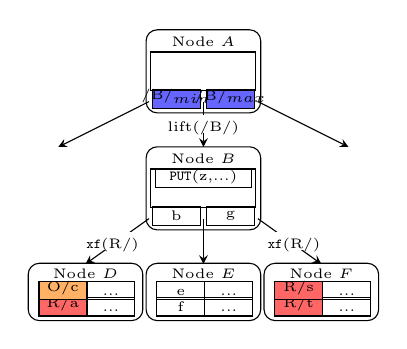
\begin{tikzpicture}[xscale=0.95, yscale=0.95]
            \node[anchor=south, rectangle, rounded corners, minimum height=.06\textwidth, minimum width=.12\textwidth, draw=black] at (.13\textwidth, 0) {};
            \node[anchor=south, font=\tiny] at (.13\textwidth, .036\textwidth) {Node $D$};
            \node[anchor=south, rectangle, minimum height=.015\textwidth, minimum width=.05\textwidth, draw=black, fill={red!60}] at (.105\textwidth, .005\textwidth) {};
            \node[anchor=south, font=\tiny] at (.105\textwidth, 0) {R/a};
            \node[anchor=south, rectangle, minimum height=.015\textwidth, minimum width=.05\textwidth, draw=black] at (.158\textwidth, .005\textwidth) {};
            \node[anchor=south, font=\tiny] at (.158\textwidth, 0) {...};
            \node[anchor=south, rectangle, minimum height=.015\textwidth, minimum width=.05\textwidth, draw=black, fill={orange!60}] at (.105\textwidth, .023\textwidth) {};
            \node[anchor=south, font=\tiny] at (.105\textwidth, .018\textwidth) {O/c};
            \node[anchor=south, rectangle, minimum height=.015\textwidth, minimum width=.05\textwidth, draw=black] at (.158\textwidth, .023\textwidth) {};
            \node[anchor=south, font=\tiny] at (.158\textwidth, .018\textwidth) {...};

            \node[anchor=south, rectangle, rounded corners, minimum height=.06\textwidth, minimum width=.12\textwidth, draw=black] at (.26\textwidth, 0) {};
            \node[anchor=south, font=\tiny] at (.26\textwidth, .036\textwidth) {Node $E$};
            \node[anchor=south, rectangle, minimum height=.015\textwidth, minimum width=.05\textwidth, draw=black] at (.235\textwidth, .005\textwidth) {};
            \node[anchor=south, font=\tiny] at (.235\textwidth, 0) {f};
            \node[anchor=south, rectangle, minimum height=.015\textwidth, minimum width=.05\textwidth, draw=black] at (.288\textwidth, .005\textwidth) {};
            \node[anchor=south, font=\tiny] at (.288\textwidth, 0) {...};
            \node[anchor=south, rectangle, minimum height=.015\textwidth, minimum width=.05\textwidth, draw=black] at (.235\textwidth, .023\textwidth) {};
            \node[anchor=south, font=\tiny] at (.235\textwidth, .018\textwidth) {e};
            \node[anchor=south, rectangle, minimum height=.015\textwidth, minimum width=.05\textwidth, draw=black] at (.288\textwidth, .023\textwidth) {};
            \node[anchor=south, font=\tiny] at (.288\textwidth, .018\textwidth) {...};

            \node[anchor=south, rectangle, rounded corners, minimum height=.06\textwidth, minimum width=.12\textwidth, draw=black] at (.39\textwidth, 0) {};
            \node[anchor=south, font=\tiny] at (.39\textwidth, .036\textwidth) {Node $F$};
            \node[anchor=south, rectangle, minimum height=.015\textwidth, minimum width=.05\textwidth, draw=black, fill={red!60}] at (.365\textwidth, .005\textwidth) {};
            \node[anchor=south, font=\tiny] at (.365\textwidth, 0) {R/t};
            \node[anchor=south, rectangle, minimum height=.015\textwidth, minimum width=.05\textwidth, draw=black] at (.418\textwidth, .005\textwidth) {};
            \node[anchor=south, font=\tiny] at (.418\textwidth, 0) {...};
            \node[anchor=south, rectangle, minimum height=.015\textwidth, minimum width=.05\textwidth, draw=black, fill={red!60}] at (.365\textwidth, .023\textwidth) {};
            \node[anchor=south, font=\tiny] at (.365\textwidth, .018\textwidth) {R/s};
            \node[anchor=south, rectangle, minimum height=.015\textwidth, minimum width=.05\textwidth, draw=black] at (.418\textwidth, .023\textwidth) {};
            \node[anchor=south, font=\tiny] at (.418\textwidth, .018\textwidth) {...};

            \node[anchor=south, rectangle, rounded corners, minimum height=.087\textwidth, minimum width=.12\textwidth, draw=black] at (.26\textwidth, .1\textwidth) {};
            \node[anchor=south, font=\tiny] at (.26\textwidth, .163\textwidth) {Node $B$};
            \node[anchor=south, rectangle, minimum height=.015\textwidth, minimum width=.05\textwidth, draw=black] at (.23\textwidth, .105\textwidth) {};
            \node[anchor=south, font=\tiny] at (.23\textwidth, .1\textwidth) {b};
            \node[anchor=south, rectangle, minimum height=.015\textwidth, minimum width=.05\textwidth, draw=black] at (.29\textwidth, .105\textwidth) {};
            \node[anchor=south, font=\tiny] at (.29\textwidth, .1\textwidth) {g};
            \node[anchor=south, rectangle, minimum height=.04\textwidth, minimum width=.11\textwidth, draw=black] at (.26\textwidth, .125\textwidth) {};
            \node[anchor=south, rectangle, minimum height=.015\textwidth, minimum width=.1\textwidth, draw=black] at (.26\textwidth, .147\textwidth) {};
            \node[anchor=south, font=\tiny] at  (.26\textwidth, .141\textwidth) {\putm(z,...)};

            \node[anchor=south, rectangle, rounded corners, minimum height=.087\textwidth, minimum width=.12\textwidth, draw=black] at (.26\textwidth, .229\textwidth) {};
            \node[anchor=south, font=\tiny] at (.26\textwidth, .292\textwidth) {Node $A$};
            \node[anchor=south, rectangle, minimum height=.015\textwidth, minimum width=.05\textwidth, draw=black, fill={blue!60}] at (.23\textwidth, .234\textwidth) {};
            \node[anchor=south, font=\tiny] at (.23\textwidth, .229\textwidth) {/B/$_{min}$};
            \node[anchor=south, rectangle, minimum height=.015\textwidth, minimum width=.05\textwidth, draw=black, fill={blue!60}] at (.29\textwidth, .234\textwidth) {};
            \node[anchor=south, font=\tiny] at (.29\textwidth, .229\textwidth) {/B/$_{max}$};
            \node[anchor=south, rectangle, minimum height=.04\textwidth, minimum width=.11\textwidth, draw=black] at (.26\textwidth, .254\textwidth) {};

            \draw[->, >=stealth] (.20\textwidth, .113\textwidth) -- (.13\textwidth, .063\textwidth);
            \draw[->, >=stealth] (.26\textwidth, .113\textwidth) -- (.26\textwidth, .063\textwidth);
            \draw[->, >=stealth] (.32\textwidth, .113\textwidth) -- (.39\textwidth, .063\textwidth);
            \draw[->, >=stealth] (.26\textwidth, .242\textwidth) -- (.26\textwidth, .192\textwidth);
            \draw[->, >=stealth] (.20\textwidth, .242\textwidth) -- (.10\textwidth, .192\textwidth);
            \draw[->, >=stealth] (.32\textwidth, .242\textwidth) -- (.42\textwidth, .192\textwidth);

            \node[anchor=north,rectangle, minimum height=.015\textwidth, minimum width=.05\textwidth, fill={white}] at (.16\textwidth, .099\textwidth) {};
            \node[anchor=north, font=\tiny] at (.16\textwidth, .102\textwidth) {\xf (R/)};
            \node[anchor=north,rectangle, minimum height=.015\textwidth, minimum width=.05\textwidth, fill={white}] at (.36\textwidth, .099\textwidth) {};
            \node[anchor=north, font=\tiny] at (.36\textwidth, .102\textwidth) {\xf (R/)};
            \node[anchor=north,rectangle, minimum height=.015\textwidth, minimum width=.08\textwidth, fill={white}] at (.26\textwidth, .228\textwidth) {};
            \node[anchor=north, font=\tiny] at (.26\textwidth, .231\textwidth) {lift(/B/)};
        \end{tikzpicture}
        \caption{\label{subfig:xf-2} To remove the \xf function, it discards
            exterior children and adds \xf functions to parent-to-child pointers
            of fringe children.}
    \end{subfigure}
    \caption[Resolving \xf functions in node flushes]{\label{fig:xf}
        During node flushes, the lifted \bedag resolves the \xf
        function associated with the parent-to-child pointer.}
\end{figure}

Figure~\ref{fig:xf} shows an example of fixing \xf functions in node flushes.
In Figure~\ref{subfig:xf-1}, the parent-to-child pointer from Node $A$ to
Node $B$ has a \xf function, \xf(``/R/'').
The key range specified by Node $A$ is (``/B/$_{min}$'',``/B/$_{max}$''), which
translates to (``/R/$_{min}$'',``/R/$_{max}$'') in Node $B$.
In Figure~\ref{subfig:xf-2}, the lifted \bedag garbage-collects exterior nodes,
Node $C$ and $G$
and adds \xf functions to pointers to fringe nodes, Node $D$ and $F$.
Also, it updates keys in Node $B$ by removing the prefix, ``/R/'',
in the \xf function.
Note, the message \putm(/G/a,...) is also removed from Node $B$
because it is out of the key range specified in Node $A$.

\section{Implementation}

\paragraph{Preferential splitting.}
Most of the additional background work in range-clone is about removing
unrelated keys and unlifted prefix data from fringe nodes, which
contain both cloned and non-cloned data.
Therefore, it is beneficial to reduce the number of fringe nodes.

The baseline \bet splits nodes evenly.
When a leaf needs to be split, the middle key is picked as the new piovt
separating the two new leaves to be generated.
A non-leaf node split can be viewed as promoting the middle pivot in the node to
the parent.

Preferential splitting generates pivots that maximizes the common prefix under
the leaf, subject to the constraint that both leaves should be at least 1/4
full.
This strategy reduces the likelihood of having fringe nodes
in a range-clone and bounds the how unbalanced leaves can be.

A naive approach would compare all keys in the range of [1/4, 3/4] of the leaf
and picking the pair of two adjacent keys that share the shortest common prefix.
But this scan can be costly.

Preferential splitting only requires the reading of two keys.
Because the shortest common prefix of adjacent keys is the same as the common
prefix of the smallest (at 1/4 of the leaf) candidate key, $k_{s}$ and
the largest (at 3/4 of the leaf) candidate key, $k_{l}$,
a good pivot can be constructed from these two keys.
In particular, preferential splitting generates a pivot that is maximum key with
prefix $p_{s}$, where $p_{s}$ that is the shortest prefix of $k_{s}$ that
contains the LCP of $k_{s}$ and $k_{l}$ and has a slash or a end-of-string as
the last character.

\paragraph{Queries.}

\section{Summary}

This chapter first describes the new interface, range-clone, that enables file
or directory renames and clones in \betrfs.
Then, it presents a range-clone implementation that finishes all works
on the critical path and transforms a lifted \bet to a lifted \bedag.
Later, it introduces \goto messages that delay tree surgery in the range-clone,
fit the implementation into the write-optimized framework of the data structure.
At last, it describes preferential splitting that reduces work needed in
tree surgery.


\chapter{Evaluation}
\label{chap:eval}

This chapter evaluates the performance of \betrfs with
range-rename (\betrfsFour) and \betrfs with range-clone (\betrfsFive).
The evaluation includes the following four aspects:
(1) performance of single file-system operations;
(2) performance of widely used applications;
(3) performance of renames;
(4) performance of clones.

\paragraph{Experimental Setup.}

All experimental results were collected on
a Dell Optiplex 790 with a 4-core 3.40 GHz Intel Core i7-2600 CPU,
4GB RAM,
and a 500 GB, 7200 SATA disk with a 4096-byte block size(Seagate Barracuda ST500DM002).
The system runs 64-bit Ubuntu server 14.04.05 on a USB stick to prevent
interference form the root file system.
\betrfsFour runs on a modified Linux-3.11.10 kernel that enlarges the size of the kernel stack,
while \betrfsFive and all other file systems run on Linux-4.9.142 kernel.
The evaluation uses ZFS 0.6.5.11 from \url{zfsonlinx.org} and
ext4, Btrfs, XFS and NILFS2 as parts of the Linux kernel.
Each experiment runs a minimum of 5 times and reports the median number.
Error bars indicate minimum and maximum numbers over all runs.
Similarly, error $\pm$ terms bound minimum and maximum numbers over all runs.
Unless noted, all benchmarks are cold-cache tests.

\section{Microbenchmarks}

\paragraph{Sequential writes and reads.}

We measure the throughput of sequentially writing and reading a file.
This benchmark first writes a 10-GiB file, 64 blocks at a time, with a
\texttt{fsync} to flush the file to disk.
Then, after cleaning the kernel page cache, the kernel reads the file from disk.

\newcommand{\addSeqPlot}[1]{
    \addplot[
        discard if not={fs}{#1},
        fill=\pgfkeysvalueof{/fs-colors/#1},
        nodes near coords=\pgfkeysvalueof{/fs-names/#1},
    ]
    plot[
        error bars/.cd,
        y dir=both, y explicit,
    ]
    table[
        x=op,
        y=median,
        y error plus expr=\thisrow{max}-\thisrow{median},
        y error minus expr=\thisrow{median}-\thisrow{min},
    ]
    {./data/seq_io.csv};
}

\begin{figure}[t]
    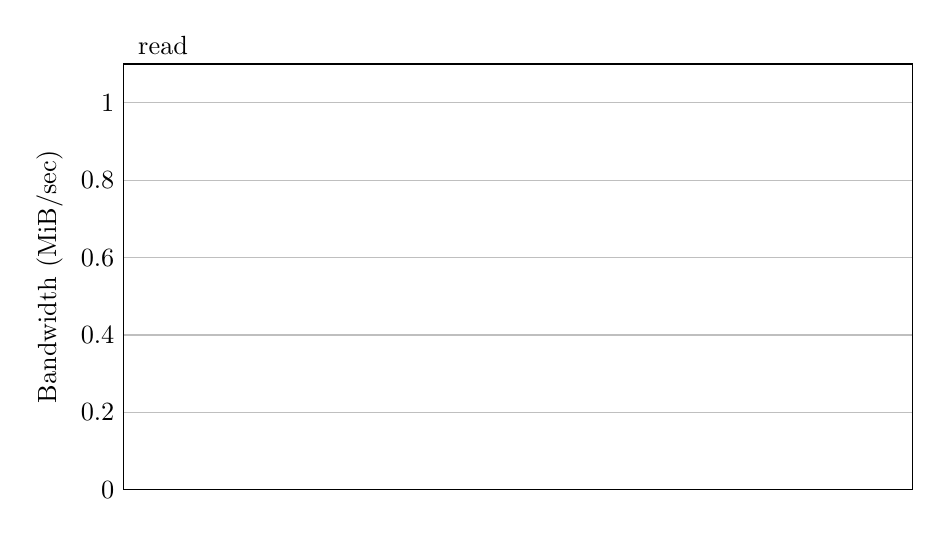
\begin{tikzpicture}[yscale=0.95, xscale=0.95]
        \begin{axis}[
                ybar,
                ymin=0,
                ylabel={Bandwidth (MiB/sec)},
                ymajorgrids=true,
                symbolic x coords={seq.write,seq.read},
                xtick={seq.write,seq.read},
                xticklabels={write,read},
                enlarge x limits=0.5,
                visualization depends on=y \as \rawy,
                xtick pos=right,
                major tick length=0in,
                xticklabel pos=right,
                nodes near coords style={font=\small,anchor=east,rotate=90,xshift=-\pgfplotsunitylength*\rawy,},
                height=.6\linewidth,
                width=\linewidth,
            ]
            \addSeqPlot{ext4};
            \addSeqPlot{btrfs};
            \addSeqPlot{xfs};
            \addSeqPlot{zfs};
            \addSeqPlot{nilfs2};
            \addSeqPlot{betrfs4};
            \addSeqPlot{betrfs5};
        \end{axis}
    \end{tikzpicture}
    \caption[Sequential-write and sequential-read benchmark]{\label{fig:seq_io}
        Bandwidth to sequentially read and write a 10 GiB file (higher is better).}
\end{figure}

Figure~\ref{fig:seq_io} shows the results.
Ext4, Btrfs, XFS performs sequential
writes close to disk bandwidth, while \betrfsFive, similar to NILFS2, is about
6.5\% slower than the fastest file system.
The performance increase of \betrfsFive from \betrfsFour is from preferential
splitting, which creates a pivot matching the maximum file data key the
beginning of the workload, avoiding further node relifting in subsequent node
splits.
For sequential reads, Ext4, Btrfs, XFS run at disk bandwidth, while \betrfsFive
is 19.1\% slower than the fastest file system, which is close to \betrfsFour
and NILFS2.
\betrfs reads a leaf, which is about 4 MiB in size, each time, while
extent-based file systems can have extents whose size is more than 100 MiB.
Thus, sequential reads results in more (and smaller) IOs on \betrfs.

\paragraph{Random writes.}

We then measure the performance of random writes on the file generated by the
sequential write benchmark.
The benchmark issues 256Ki 4-Byte overwrites (in total 1 MiB data) at random
offsets within the 10GiB file, followed by an \texttt{fsync}.

\newcolumntype{.}{D{.}{.}{-1}}

\begin{table}[t]
    \centering
    \begin{tabular}{l.@{${}\pm{}$}.}
        \hline
        File system & \multicolumn{2}{c}{random write (sec)} \\
        \hline
        \input{./data/rand_io.csv}
        \hline
    \end{tabular}
    \caption[Random-write benchmark]{\label{tab:rand_io}
        Time to perform 256Ki 4-Byte random writes one a 10GiB file.}
\end{table}

Table~\ref{tab:rand_io} shows the results.
Because \betrfs performs upserts, which doesn't read the old data, for random
writes, performing the 1MiB random writes only takes about 5 seconds on
\betrfsFour and \betrfsFive.
However, it takes at least 2022 seconds on other file file systems, which is
more than 400 times slower. 

\section{Macrobenchmarks}

\section{Rename benchmarks}

\textbf{TODO}

\section{Clone benchmarks}

\textbf{TODO}

\section{Summary}


\chapter{Conclusion}
\label{chap:conclusion}

File systems faced trade-offs between the performance of namespace
operations and spatial locality.
On one hand, traditional inode-based file systems have good performance for namespace
operations because of the indirection between a directory and entries under it.
However, this indirection stops these file systems from grouping metadat and data
under one directory close to each other on disk,
especially when the file system ages.
On the other hand, full-path-indexed file systems ensure locality by indexing
metadata and data by full-paths.
However, existing full-path-indexed file systems either have unbounded I/O costs for
namespace operations, or taxes other operations for efficient namespace operations.

This dissertation first presents a new operation on \bets, range-rename,
that updates all keys with one prefix to have another prefix.
The range-rename operation adopts \textbf{key lifting} to transform \bets into
lifted \bets
and accomplishes its task in a bounded number of I/Os through
\textbf{tree surgery}.
By invoking range-rename operations for file system renames,
full-path-indexed \betrfs has bounded I/O costs for its renames.

Then, this dissertation introduces another new operation on \bets, range-clone,
that clones all keys with one prefix to have another prefix.
By transforming lifted \bets into lifted \bedags, range-clone can utilize
the techniques introduced by range-rename to complete its work on the critical path.
Moreover, the range-clone operation can delay the tree surgery work with a new
type of messages, \goto messages, fitting itself into the write-optimized
framework of \bedags.
Full-path-indexed \betrfs thus has write-optimized file or directory renames and
clones by implementing them with range-clone operations.

This dissertation shows that with the right optimizations, a full-path-indexed,
write-optimized file system can
have both efficient namespace operations and locality.
There is no trade-off between them.
Also, full-path indexing opens up new opportunities for namespace operations,
such as directory clones.



% The graduate school Format Guide put endnotes before appendixes But the
% provided sample pages put appendixes before endnotes It's unclear which one
% is correct. Recommend to use footnotes instead of endnotes.
%\appendix
%\chapter{Example Appendix}
\label{chap:appendix}
\lipsum[1]

\chapter{Another Appendix}
\label{chap:appendix2}

\lipsum[1]

\clearpage

%\begin{center}
\vspace*{46pt}
\currentpdfbookmark{ENDNOTES}{bk:endnotes}
\textbf{ENDNOTES}
\vspace{10pt}
\end{center}
\addcontentsline{toc}{chapter}{ENDNOTES}

\theendnotes{}

\clearpage


\clearpage
\phantomsection

{\def\chapter*#1{} % suppress bibliograph header.
\begin{singlespace}
\addcontentsline{toc}{chapter}{REFERENCES}
\begin{center}
\textbf{REFERENCES}
\vspace{17pt}
\end{center}

\bibliographystyle{apalike}
\bibliography{references}
\end{singlespace}
}


\end{document}
